% vim: tw=80

\chapter{Theory Predictions for the Triple-Differential Dijet Cross Section}

Point like parton-parton scattering in high energy collisions can produce
jets with large transverse momenta. Events containing two such jets  in the
final state (dijet events) allow for rigorous tests of perturbative Quantum
Chromodynamics (pQCD) predictions and can subsequently be used to better
constrain the proton PDFs and extract Standard Model parameters like the strong
coupling constant~\as.

Since quite a while, next-to-leading-order (NLO) pQCD predictions are available
for jet and multijet observables. These accurately describe shape and
normalization of jet cross sections, though still suffer from larger scale
uncertainties limiting the precision of Standard Model parameters extracted from
measurements.

For almost ten years, theorists have been working on improving the jet cross
section predictions and providing next-to-next-to-leading-order (NNLO) corrections for
dijet calculations. When these corrections are publicly available, they will
push the precision of pQCD jet cross section predictions to a new level.

With the finalization of this huge project steadily approaching, we provide a
measurement which is specifically designed to benefit from these improvements.
The aim of this measurement is the determination of the proton PDFs with high
precision by using dijet events with large transverse momenta.

\section{Cross Section Definition}

The partons involved in the scattering process are assumed to be massless and
collinear to the beam protons. Most information about the initial-state partons
is gained by differentially measuring the rapidities of the two outgoing jets
and the energy of the jets. At leading order, the jet rapidities are directly
related to accessed momentum fractions in the proton via

\begin{equation*}
    x_1 = \frac{x_\mathrm{T}}{2} \left( e^{y_1} + e^{y_2} \right)
    \qquad\text{and}\qquad x_2 = \frac{x_\mathrm{T}}{2} \left( e^{-y_1} +
    e^{-y_2} \right)
\end{equation*}
with $x_{\mathrm{T}} = \sfrac{\pt}{E}$ and the rapidities of the two outgoing
partons $y_1$ and $y_2$.

However by explicitly binning the measurement in the leading and second jet, a
dependence on the ordering of the jets is introduced. While the ordering of the
jets is irrelevant at leading order since both jets are perfectly balanced and
have the same transverse momentum, it becomes relevant at NLO. The order of the
jets can be changed by a soft emission causing a different dijet ordering.
Simply put, the second jet can become the leading jet and vice versa.  Thus it
is not guaranteed that all divergences are cancelled and the observable is as a
consequence infrared unsafe.  This can be overcome by filling all histograms
twice with interchanged leading and second jet. However this produces
correlations between phasespace regions far off and unneccesary complicates the
measurement, especially the unfolding procedure.

Therefore a different definition of the cross section is chosen in this
analysis. Instead of using the rapidities and the transverse momenta of each
jet, variables which are symmetric between permutations of the leading two jets
are used. Since these observables are linear combinations of the jet rapidities,
no information is lost.

The longitudinal boost of the parton-parton center-of-mass (CM) frame with
respect to the proton-proton CM frame, \yboost, is calculated from the
rapidities $y_1$ and $y_2$ of the two jets emerging from the partons. 

\begin{equation*}
    \yboost = \frac{1}{2} |y_1 + y_2|
\end{equation*}

The quantities $\pm\ystar$ are the jet rapidities of the two jets in the
parton-parton CM frame. Since they are symmetric \ystar is defines as half the
absolute rapidity separation between the two jets.

\begin{equation*}
    \ystar = \frac{1}{2} |y_1 - y_2|
\end{equation*}
\ystar is related to the polar scattering angle $\theta$ with respect to the
beamline by 

\begin{equation*}
    \ystar = \frac{1}{2} \left( \frac{1 + |\cos \theta|}{1- | \cos \theta|}
    \right)
\end{equation*}

The triple-differential cross sections are measured as a function of the average dijet
transverse momentum $\ptavg = \frac{p_{\mathrm{T},1} + p_{\mathrm{T},2}}{2}$ and
are binned in the variables \ystar and \yboost. $p_{\mathrm{T},1}$ and
$p_{\mathrm{T},2}$ depict the transverse momenta of the two leading jets. 

The binning in those two variables has the additional advantage, that the
measurement also separates between same side (SS) and opposite side (OS) dijet
events. Fig.~\ref{fig:ysyb_schema} contains a descriptive representation of the
dijet topologies in the various \ystar and \yboost bins. If the rapidity
separation and the boost of the dijet event is small, both jets must have a low
rapidity, see bottom left plot. If the dijet system is boosted but the two jets
have a small separation in rapity, they must be boosted in the forward region to
the same side, see bottom right plot. If instead the separation is large and the
boost of the dijet system is small, then the jets must be boosted to opposide
sides. Dijet events with both a large rapidity separation and a large boost of
the dijet system are suppressed in the accessible phase space.

\begin{figure}[htbp]
    \centering
    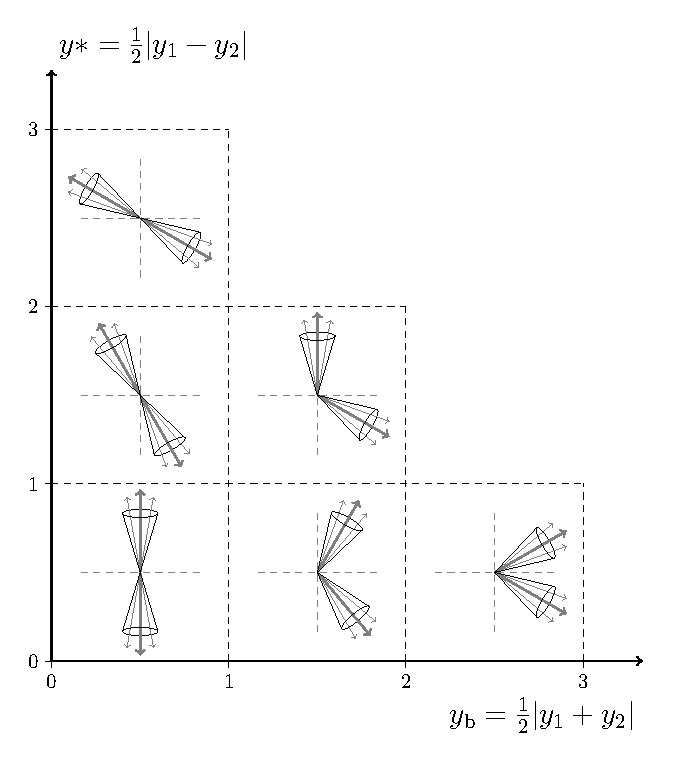
\includegraphics[width=0.9\textwidth]{figures/measurement/ybys.pdf}
    \caption{A descriptive representation of the dijet topologies in the various
    \ystar and \yboost bins. The binning separates in same side dijet
    events and opposite side dijet events which allows to draw conclusions about
    the initial state parton properties.}
    \label{fig:ysyb_schema}
\end{figure}

The differentiation in SS and OS dijet events is especially interesting since
both event topologies must access different fractional proton momenta while the
jets manifest themselves in the same (forward) detector region. Therefore
differences in the predictions can be attributed to the PDFs. This is clearly
visible in Fig.~\ref{fig:pdf_uncertainties} which shows the PDF uncertainties of
the cross section calculations. The measurement bin containing the events with
the large rapidity separation, see bottom right plot, has a significant larger
PDF uncertainty since there the high fractional proton momenta are accessed,
which are not well known.

\section{Fixed Order NLO Prediction}

The NLO cross section of the triple-differential dijet cross section is
calculated using fastNLO~\cite{Kluge:2006xs,Britzger:2012bs}. The fastNLO
interpolation tables are filled with the perturbative coefficients of the
\NLOJETPP program~\cite{Nagy:2003tz}, see Sec.~\ref{sec:nlojetpp}. The PDFs are
accessed via the LHAPDF library~\cite{Whalley:2005nh,Buckley:2014ana}. The
\as-evolution is done using the routines provided by the PDF sets. The advantage
of the application of the fastNLO framework instead of direct calculation using
\NLOJETPP is the possibility to repeat the calculations using different PDFs and
scale choices as it is neccessary to calculate the PDF and scale uncertainties.

\subsection{Scale Choice}
\label{sec:scale_coice}

Within perturbative cross section calculations, one has to choose a
factorization scale \muf and a renormalization scale \mur. The influence of these scales vanishes
when the calculation is performed for all orders of the perturbative series.
However since the perturbative series is truncated at NLO, a scale dependence on our result is
remains. Three possibilities for the scale choice are studied in this thesis.
The most natural scale choice which reflects the energy scale of the measurement
is the average \pt of the dijet system as it is also used as observable. 

\begin{equation*}
    \mu = \mur = \muf = \frac{p_{\mathrm{T},1} + p_{\mathrm{T},2}}{2}
\end{equation*}

While this scale choice yields reasonable results, the $k$-factors and scale
uncertainties indicate problems, which are discussed in detail
in Sec.~\ref{sec:k_factors} and Sec.~\ref{sec:scale_uncertainties}. The second investigated scale choice is based on the
findings of a recent analysis by ATLAS~\cite{Aad:2011fc}. They claim that
fixed-order calculations which are binned in the rapidity separation \ystar
become  unreliable for high values of
\ystar if the scale choice only depends on the energy. Based on recommendations
by theorists~\cite{Ellis:1992en}, a scale which also introduces a dependence on
the rapdity separation is proposed.
\todo{more motivation}

\begin{equation*}
    \mu = \mur = \muf = p_{\mathrm{T,max}} e^{0.3 \ystar} 
\end{equation*}

Furthermore a variation of this scale choice is studied in which the scale is not
dependent on the transverse momentum of the leading jet but on the average
transverse momentum of the leading two jets as this again resembles the
observable in this measurement.

\begin{equation*}
    \mu = \mur = \muf = p_{\mathrm{T,avg}} e^{0.3 \ystar} 
\end{equation*}

Fig.~\ref{fig:xs_nlo_comp} shows the predictions of the NLO calculation using
the three discussed scale choices. The cross section predicted by each of
calculations is similar with larger deviations for the scale choice using the
maximum transverse momentum instead of the average dijet transverse momentum.
The differences between the predictions however are covered by the scale uncertainties
afflicted to themselves.

\begin{figure}[htp]
    \centering
    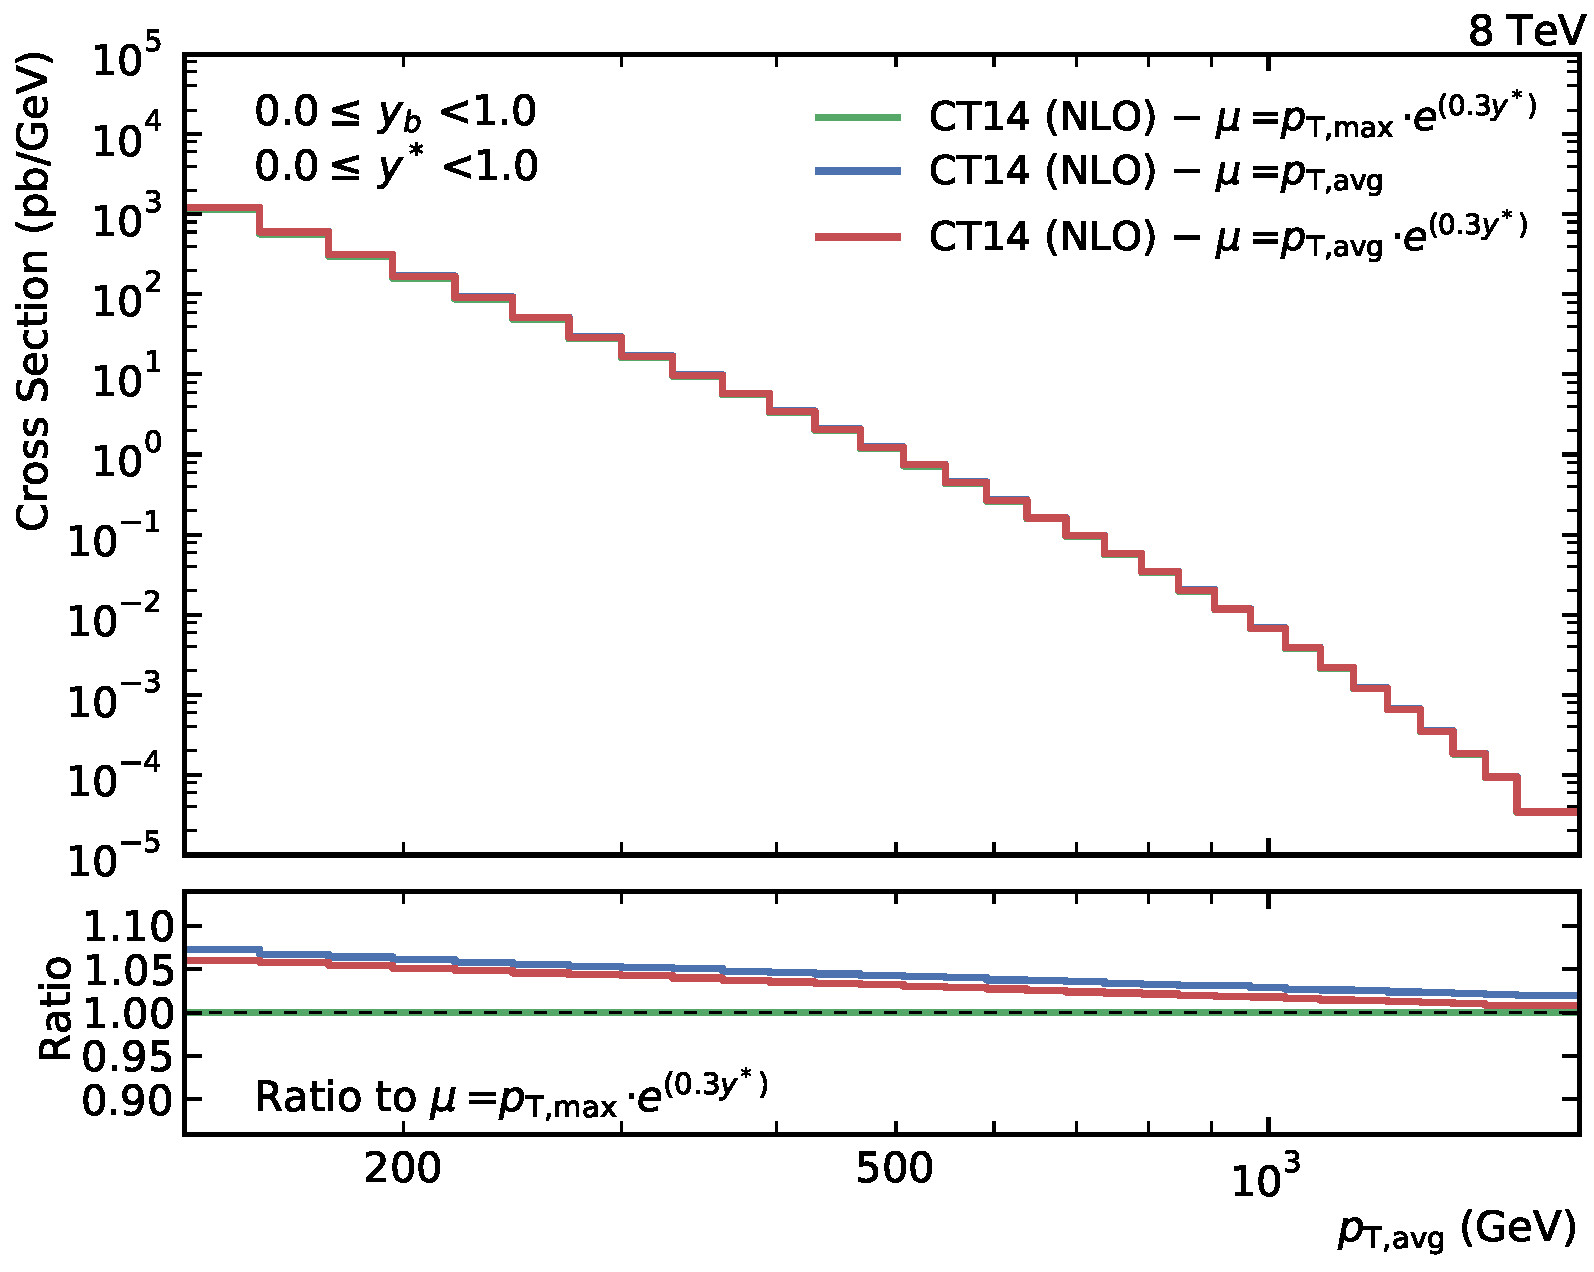
\includegraphics[width=0.45\textwidth]{figures/theory/nlo_xs_comp_yb0ys0.pdf}\hfill
    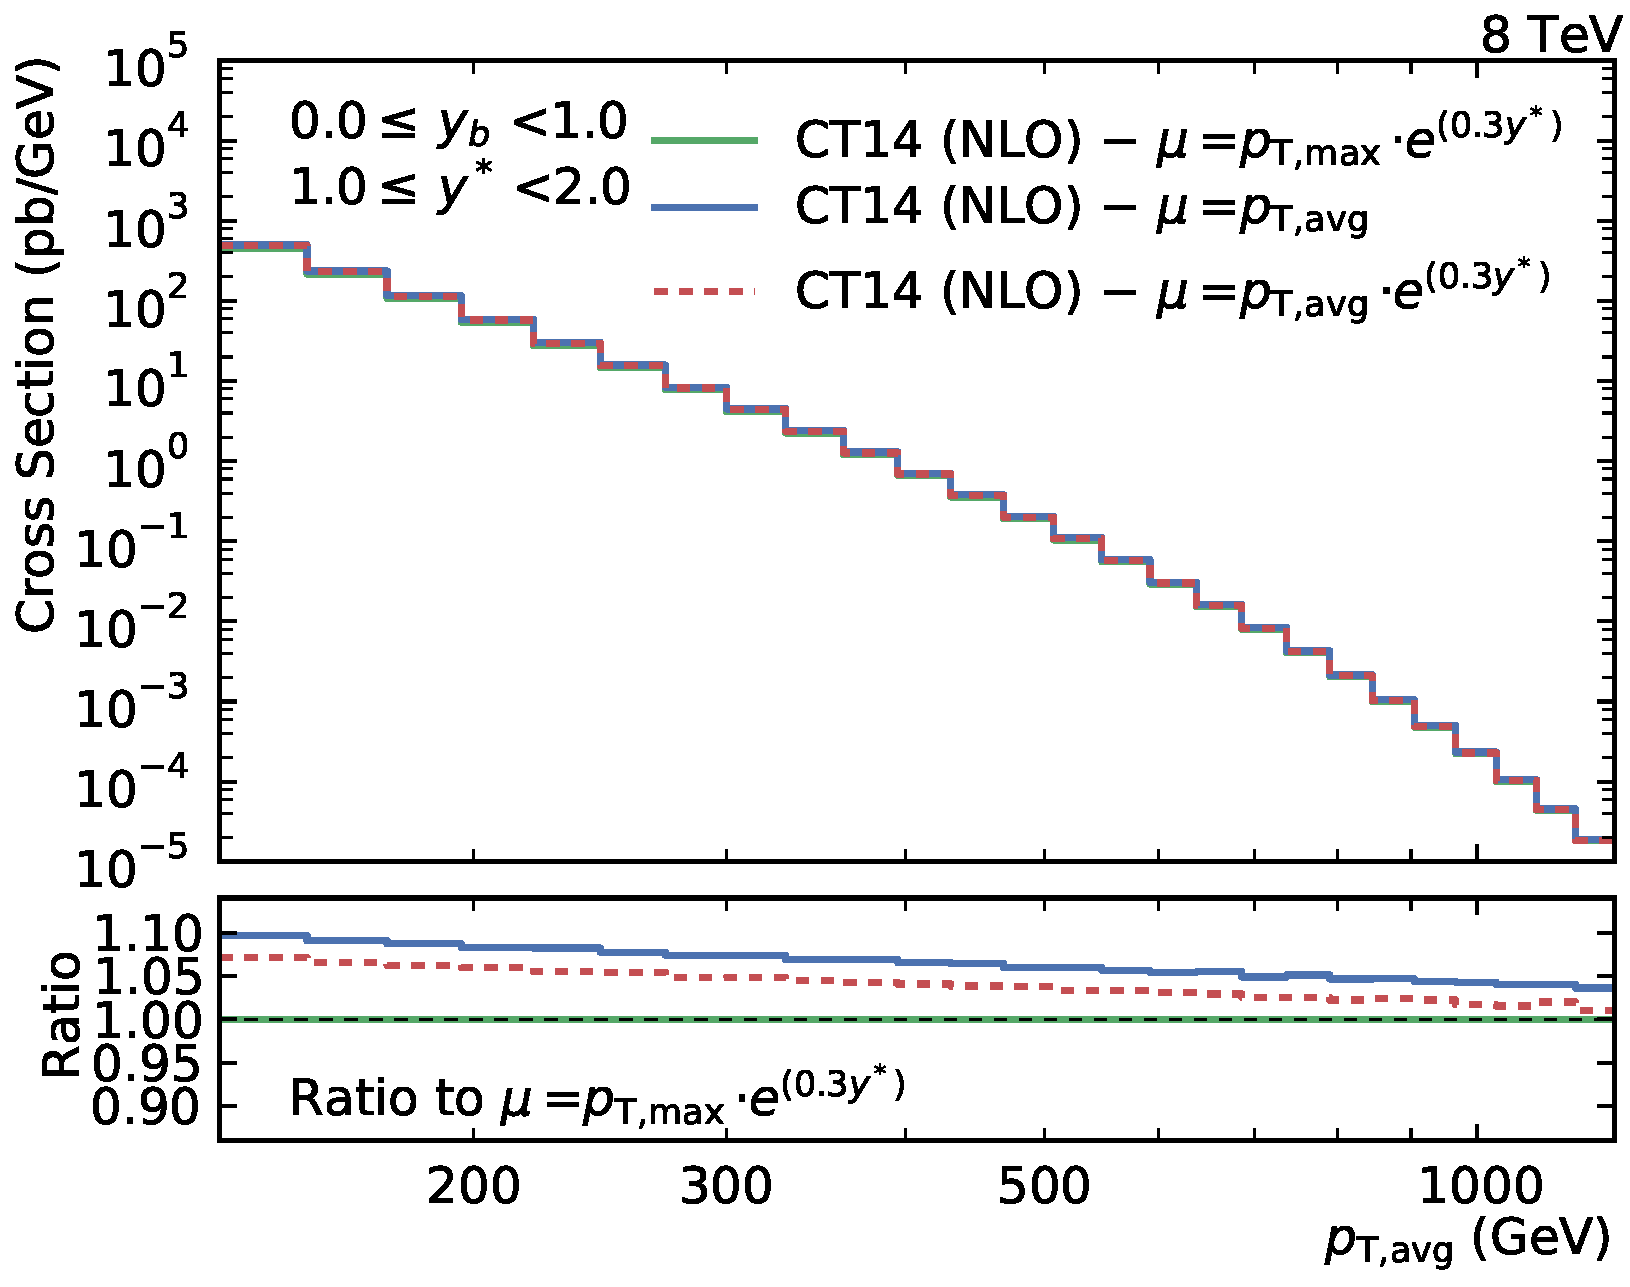
\includegraphics[width=0.45\textwidth]{figures/theory/nlo_xs_comp_yb0ys1.pdf}
    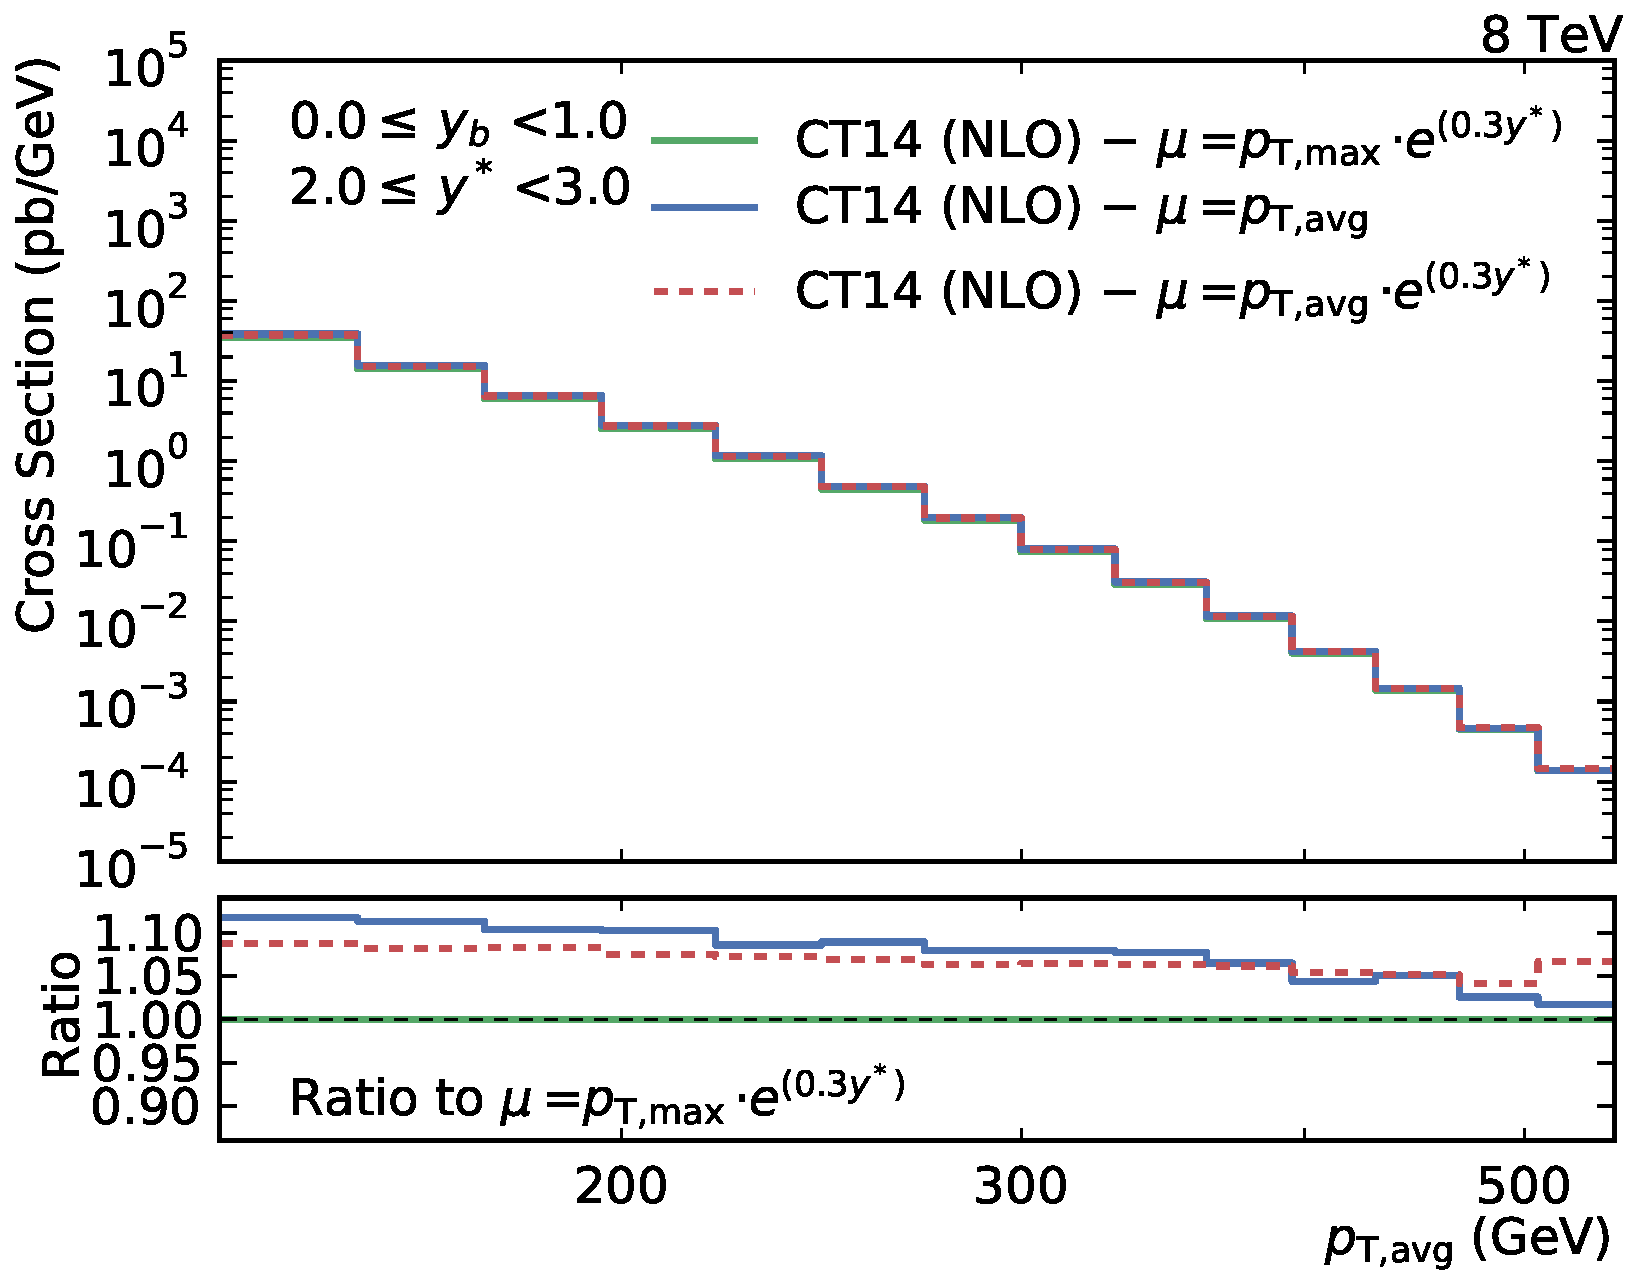
\includegraphics[width=0.45\textwidth]{figures/theory/nlo_xs_comp_yb0ys2.pdf}\hfill
    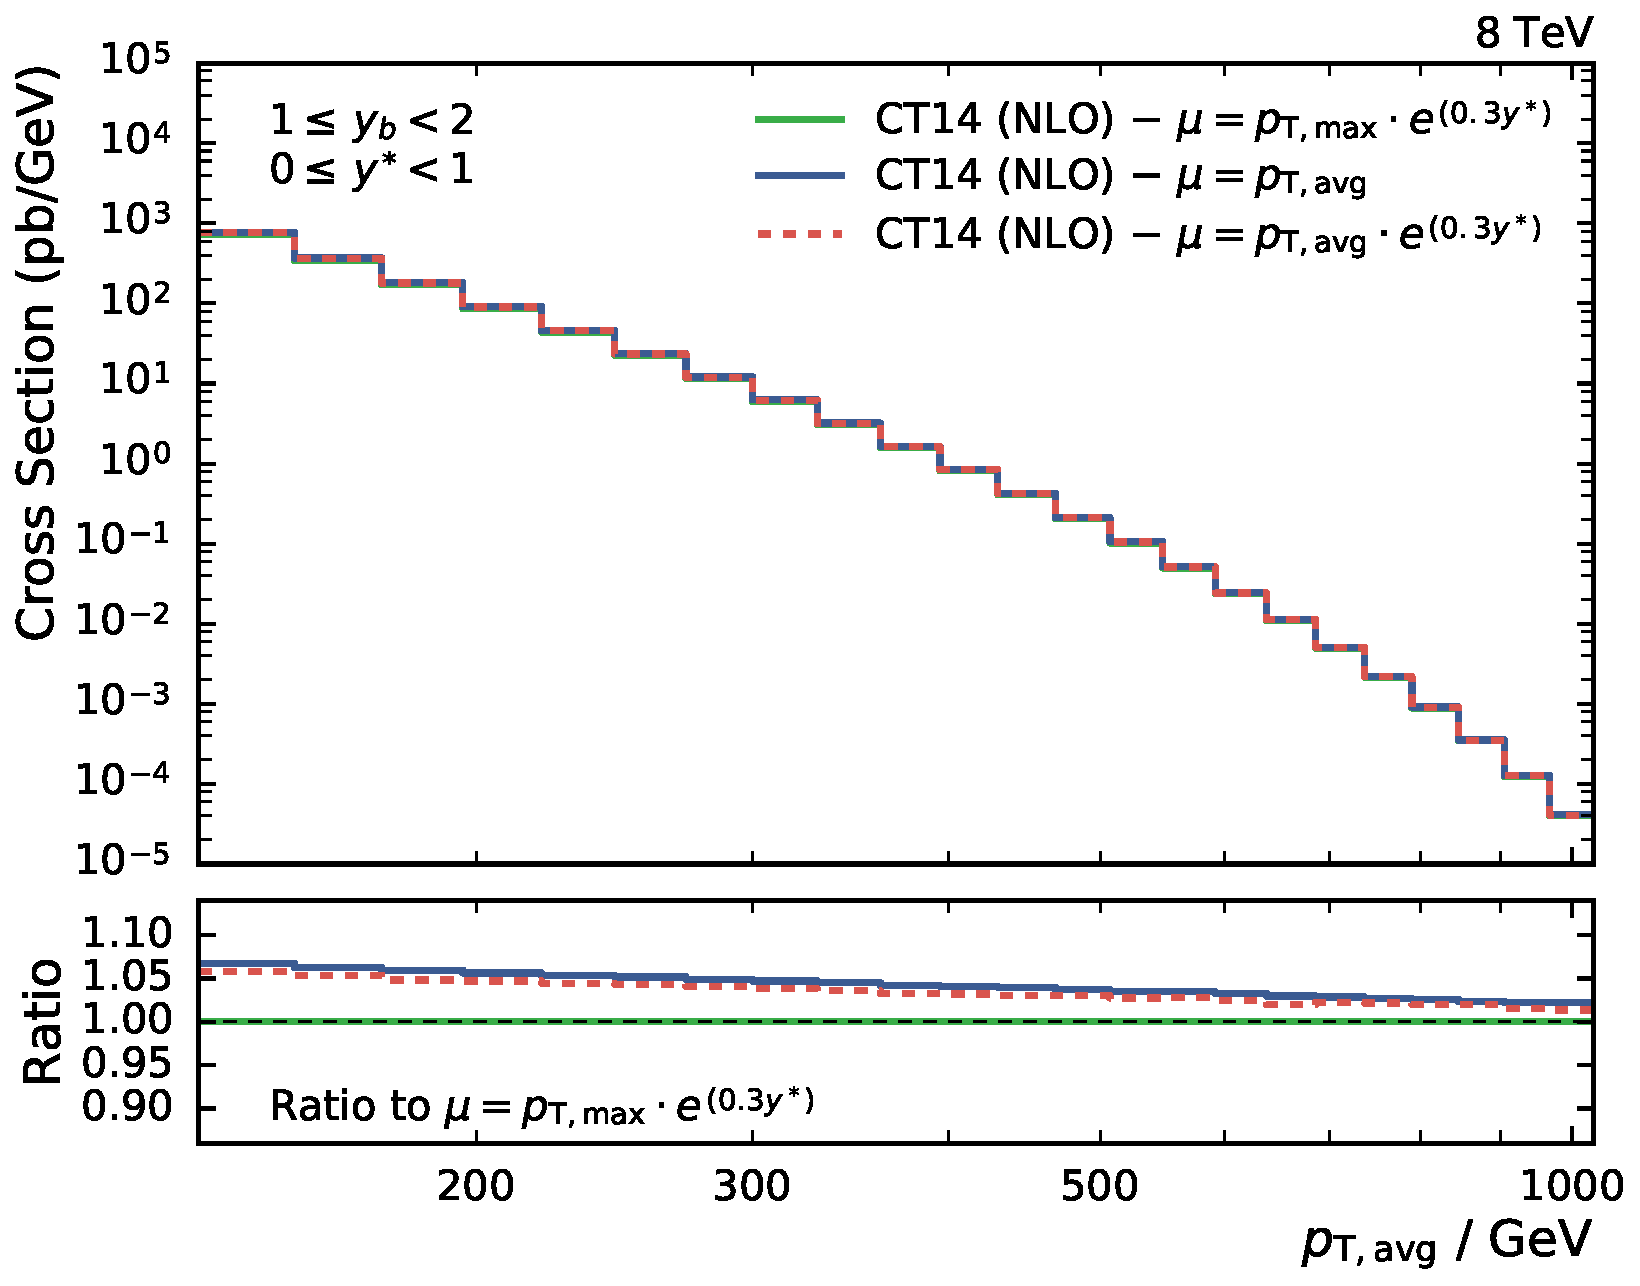
\includegraphics[width=0.45\textwidth]{figures/theory/nlo_xs_comp_yb1ys0.pdf}
    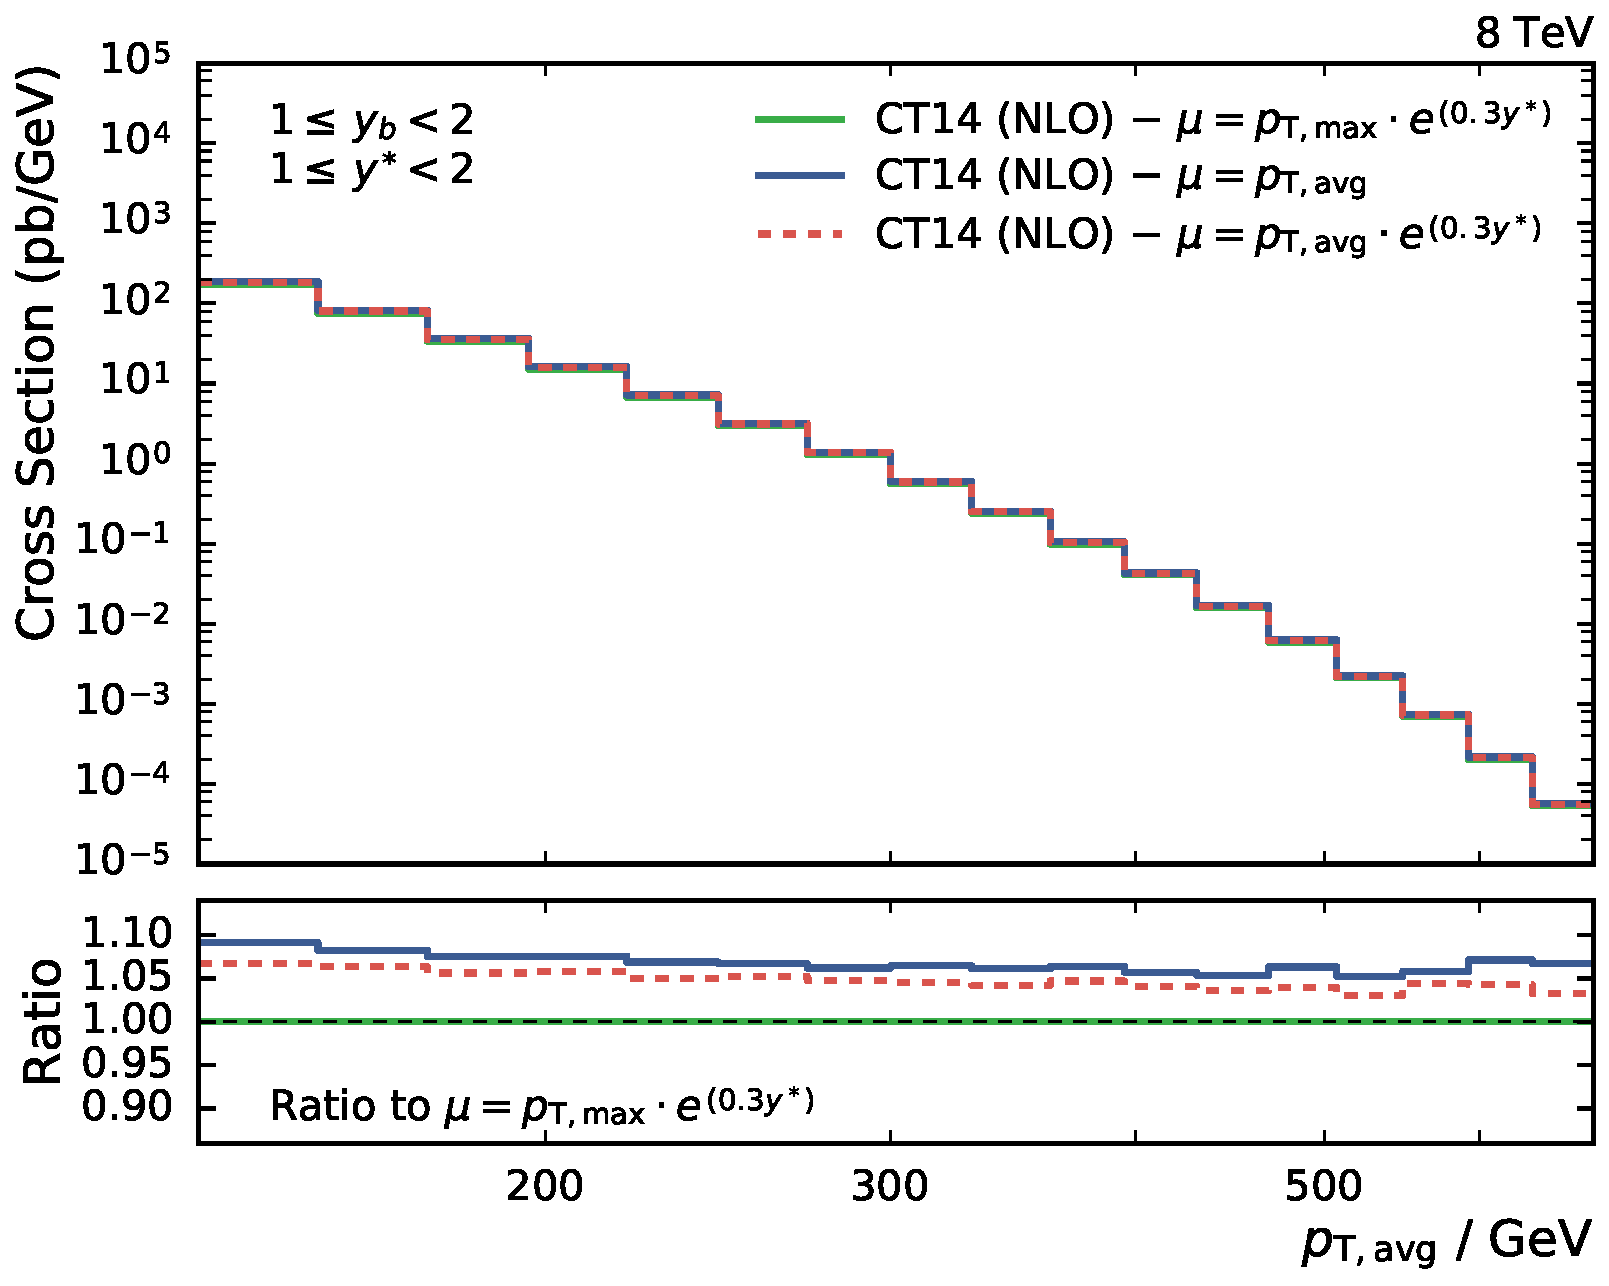
\includegraphics[width=0.45\textwidth]{figures/theory/nlo_xs_comp_yb1ys1.pdf}\hfill
    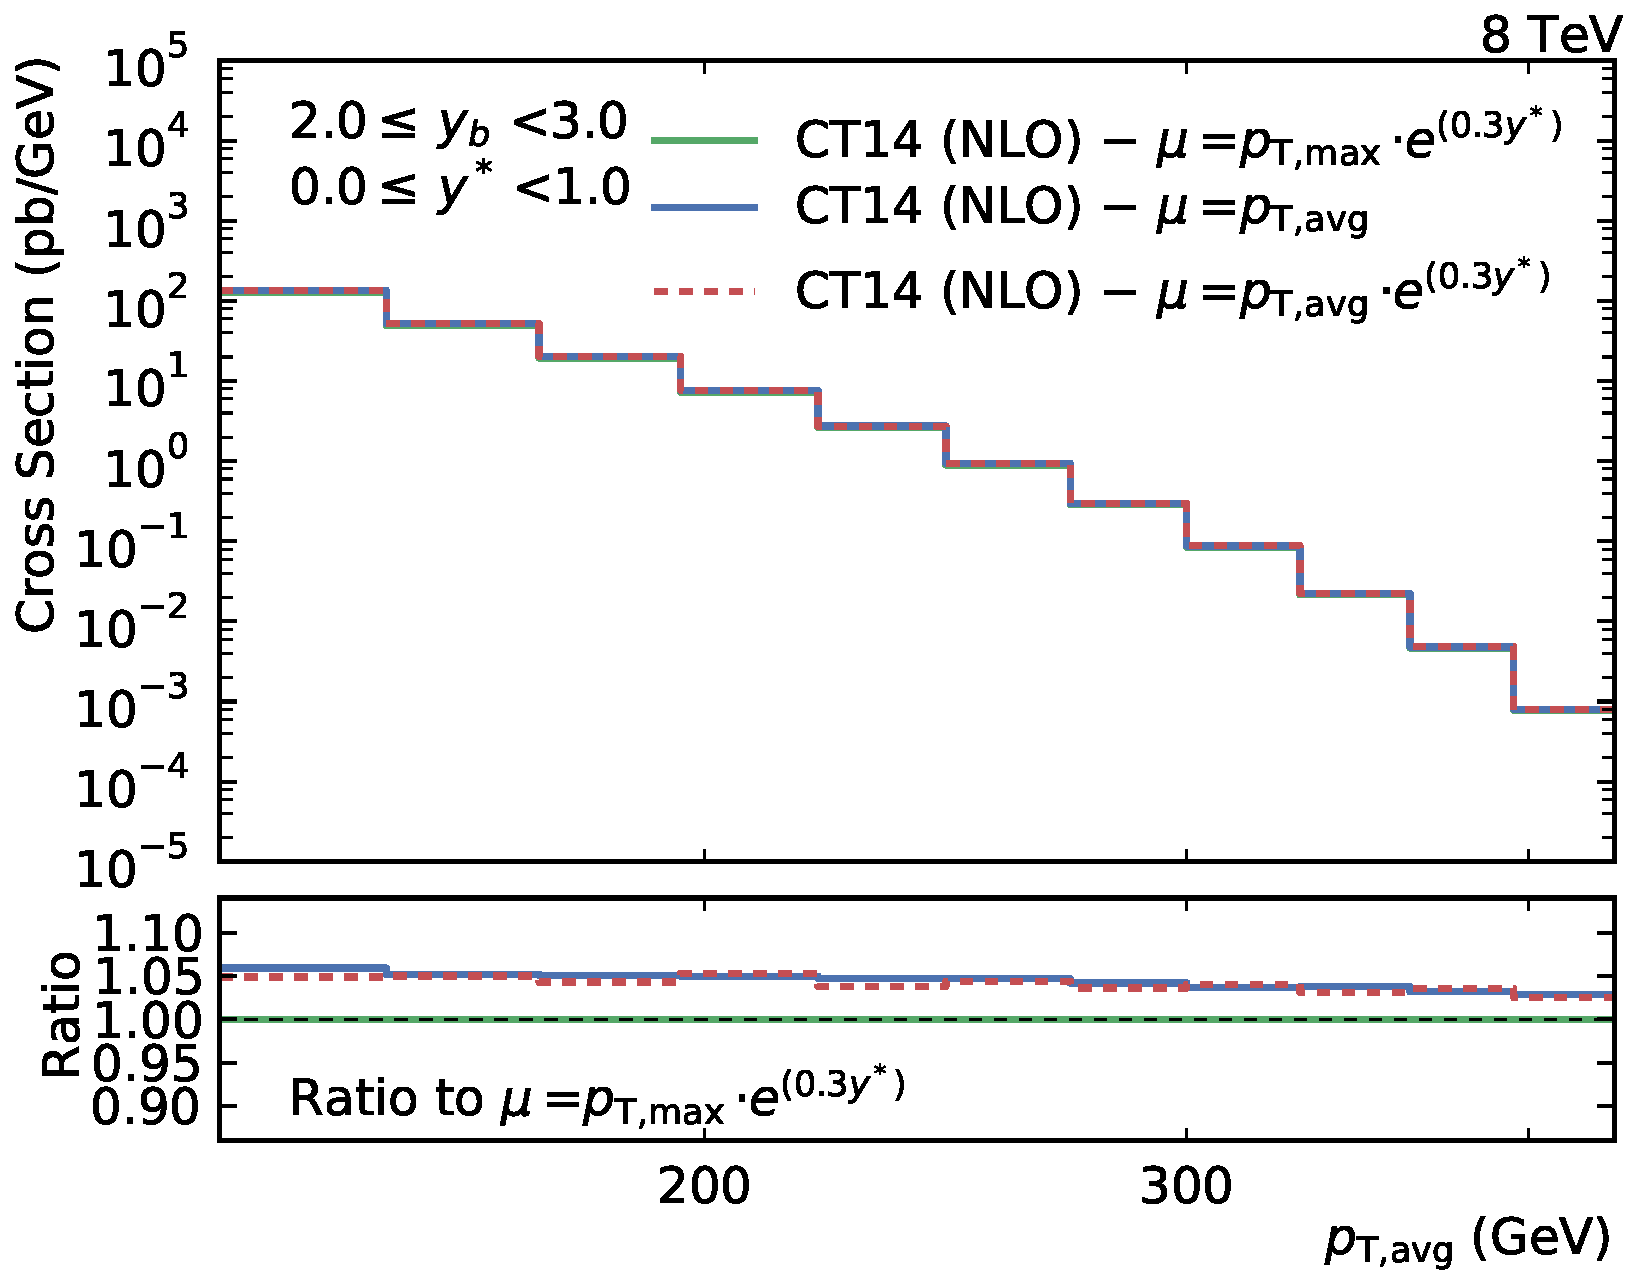
\includegraphics[width=0.45\textwidth]{figures/theory/nlo_xs_comp_yb2ys0.pdf}
    \caption{The NLO predictions of \fastNLO interfaced to \NLOJETPP for the
        triple-differential dijet measurement. The
    calculations using three different scale choices are shown. In almost all cases
    the differences between the calculations are covered by the scale
    uncertainties, see Sec.~\ref{sec:scale_uncertainties}.}
    \label{fig:xs_nlo_comp}
\end{figure}


\subsection{NLO Correction Factors}
\label{sec:k_factors}

To check the influence of higher-order contributions to the perturbative QCD
prediction, one calculates the differences between the LO prediction and the NLO
prediction, expressed as the ratio $k_\mathrm{NLO}$.

\begin{equation*}
    k_{\mathrm{NLO}} = \frac{\sigma_{\mathrm{NLO}}}{\sigma_{\mathrm{LO}}}
\end{equation*}

The size of the NLO correction gives an estimation about the influence of these
higher-order corrections. If they are small, the LO result already describes the
observable cross section precisely. It is also possible that the $k$-factors
fall below unity, in which the NLO corrections are negative and the total cross
section decreases when adding the correction.  Fig.~\ref{fig:kfactor_comp} shows
the $k$-factors of the \NLOJETPP cross section calculations using the discussed
scale choices in Sec.~\ref{sec:scale_coice}. The $k$-factors are similar in the
central region, but become quite different in regions with larger rapidity
separations.  Especially the $k$-factors in the phase space region with a
rapidity separation of $2.0 \leq \ystar < 3.0$ are smaller than unity for the
\ptavg scale choice while it is larger than one for the scale choices including
the \ystar dependence.

Apart from the findings for the \ptavg scale choice, the $k$-factors are
reliable and as expected from previous studies.

\begin{figure}[htp]
    \centering
    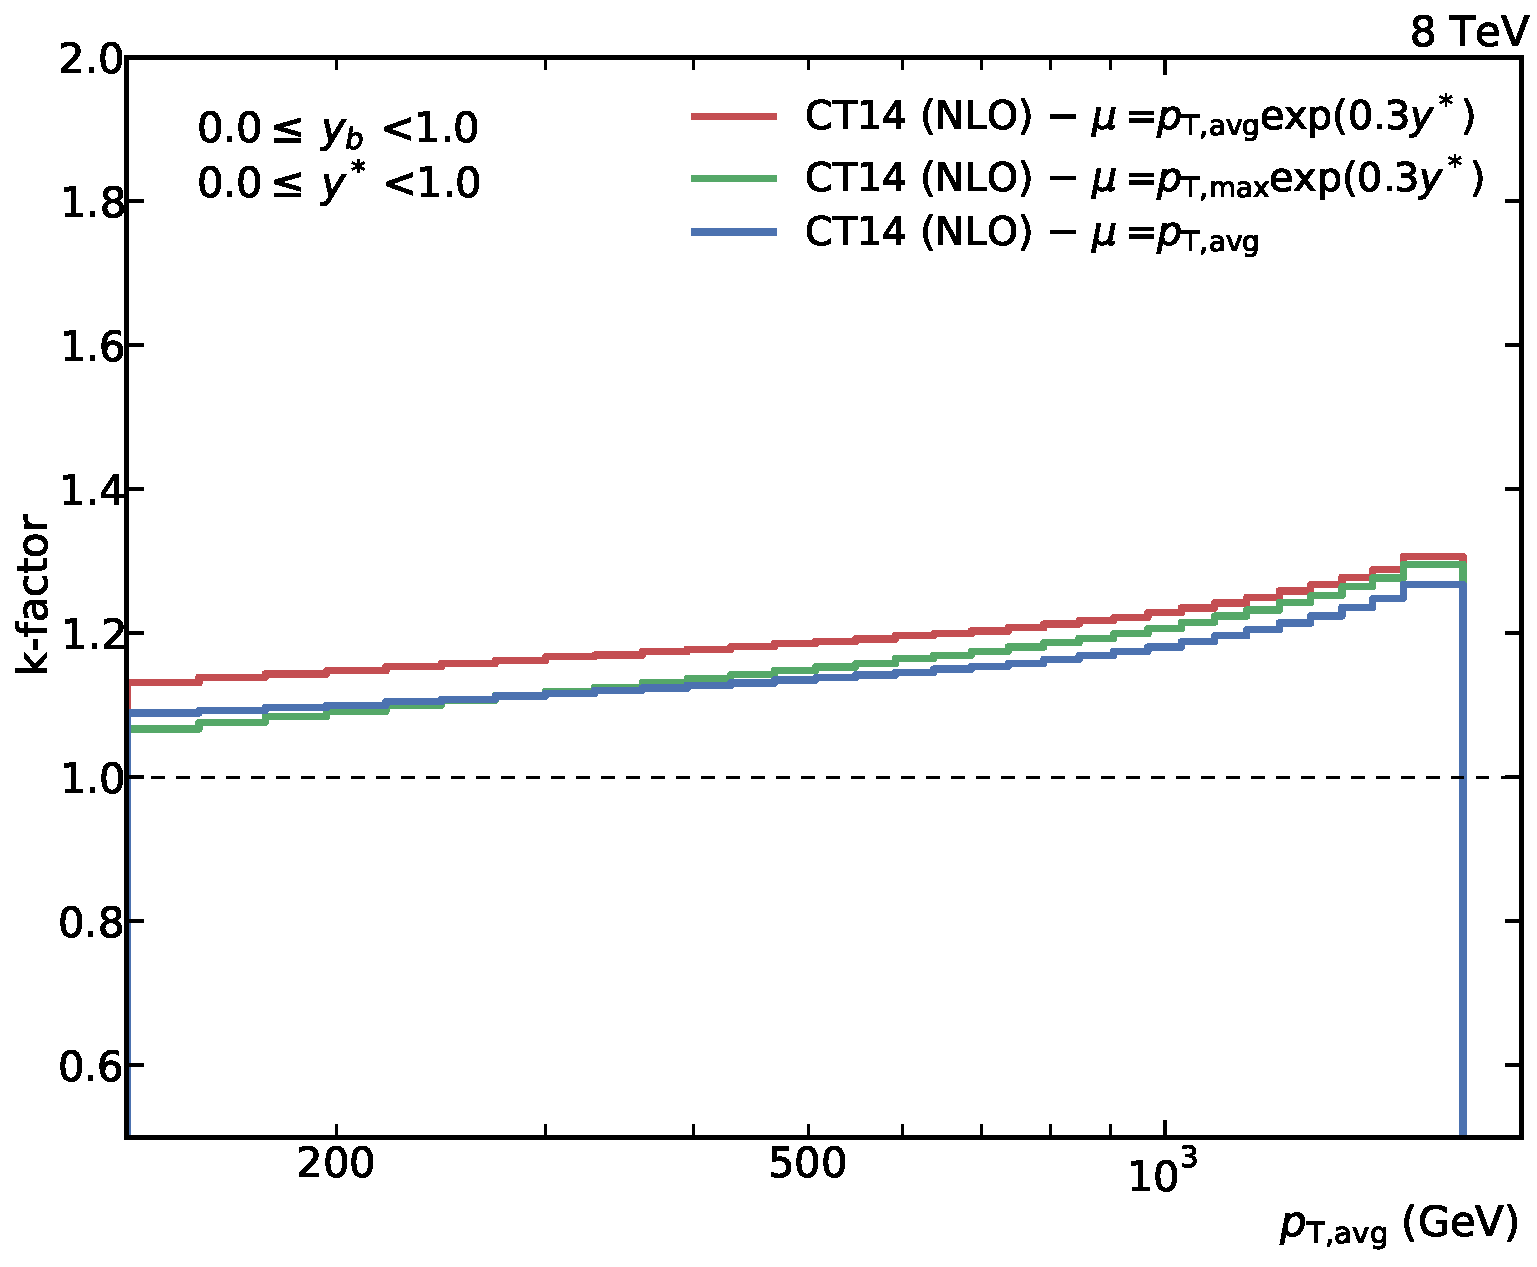
\includegraphics[width=0.45\textwidth]{figures/theory/kfactor_comp_yb0ys0.pdf}\hfill
    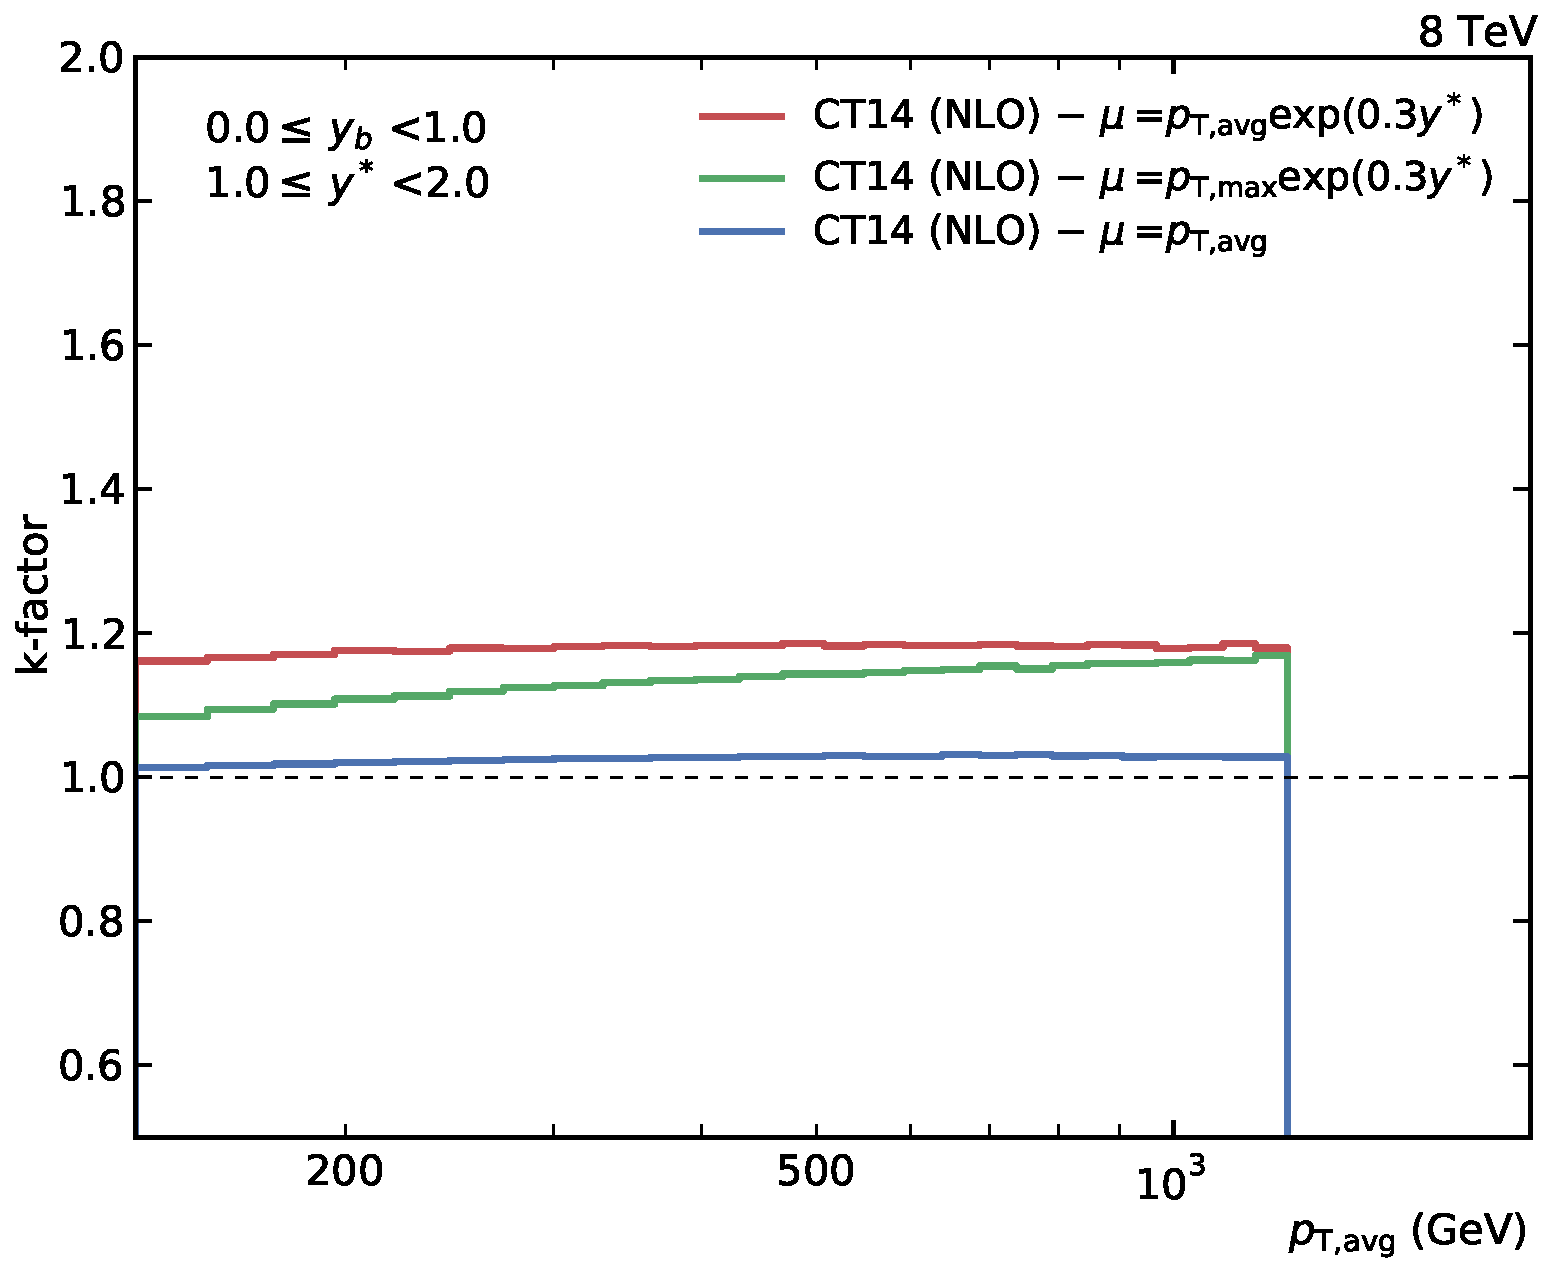
\includegraphics[width=0.45\textwidth]{figures/theory/kfactor_comp_yb0ys1.pdf}
    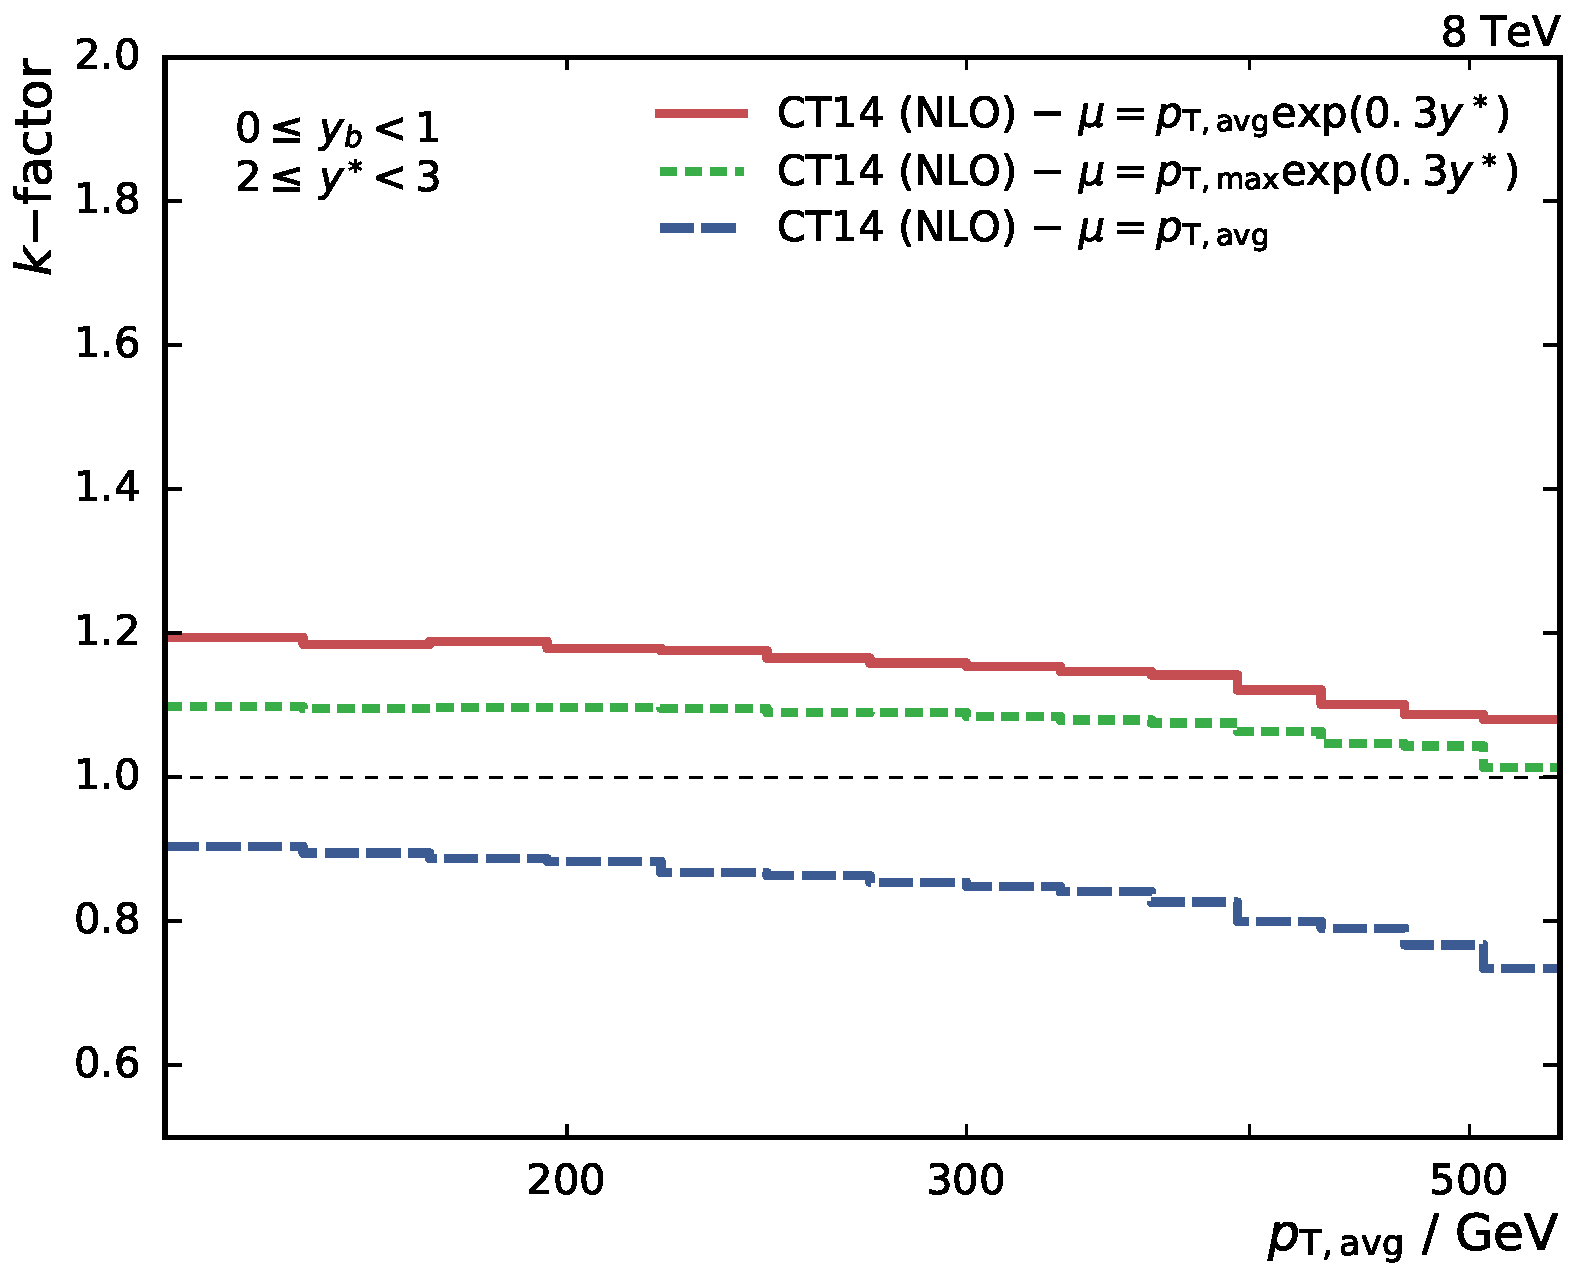
\includegraphics[width=0.45\textwidth]{figures/theory/kfactor_comp_yb0ys2.pdf}\hfill
    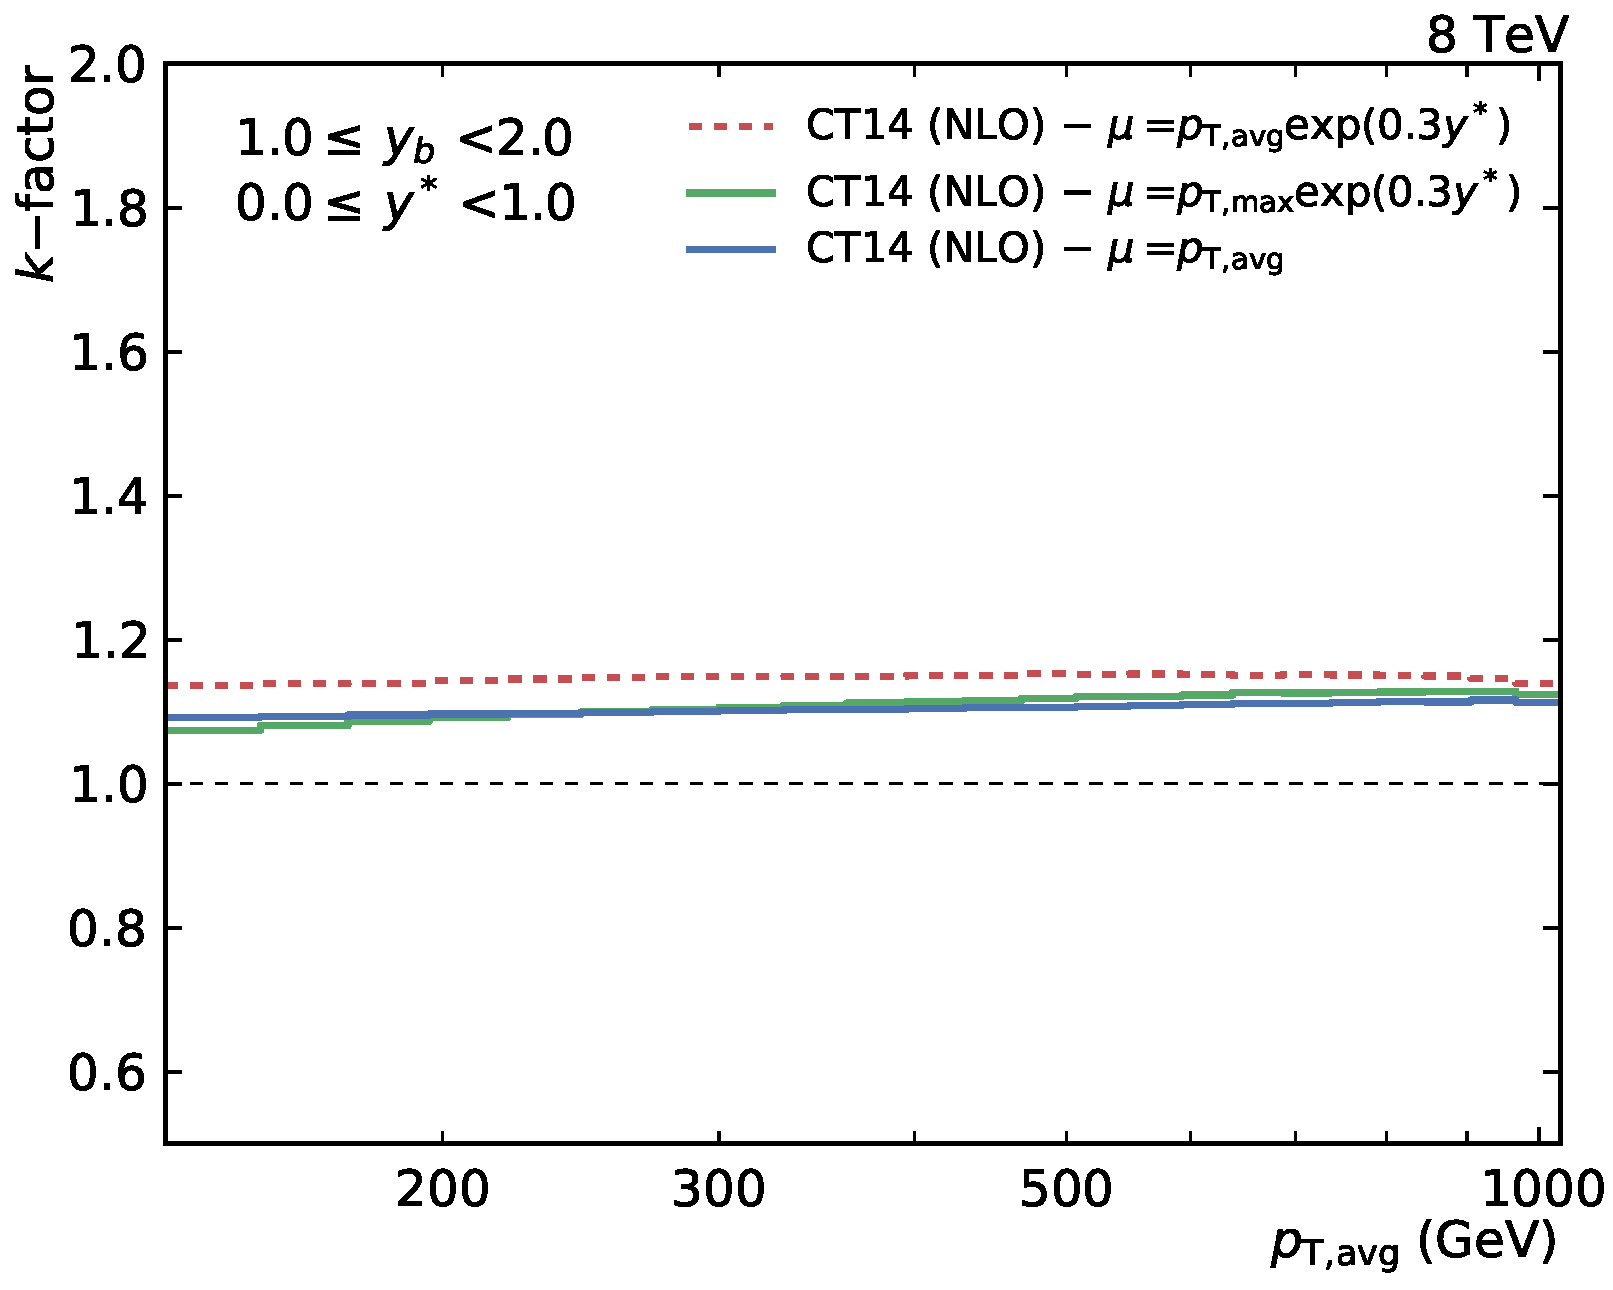
\includegraphics[width=0.45\textwidth]{figures/theory/kfactor_comp_yb1ys0.pdf}
    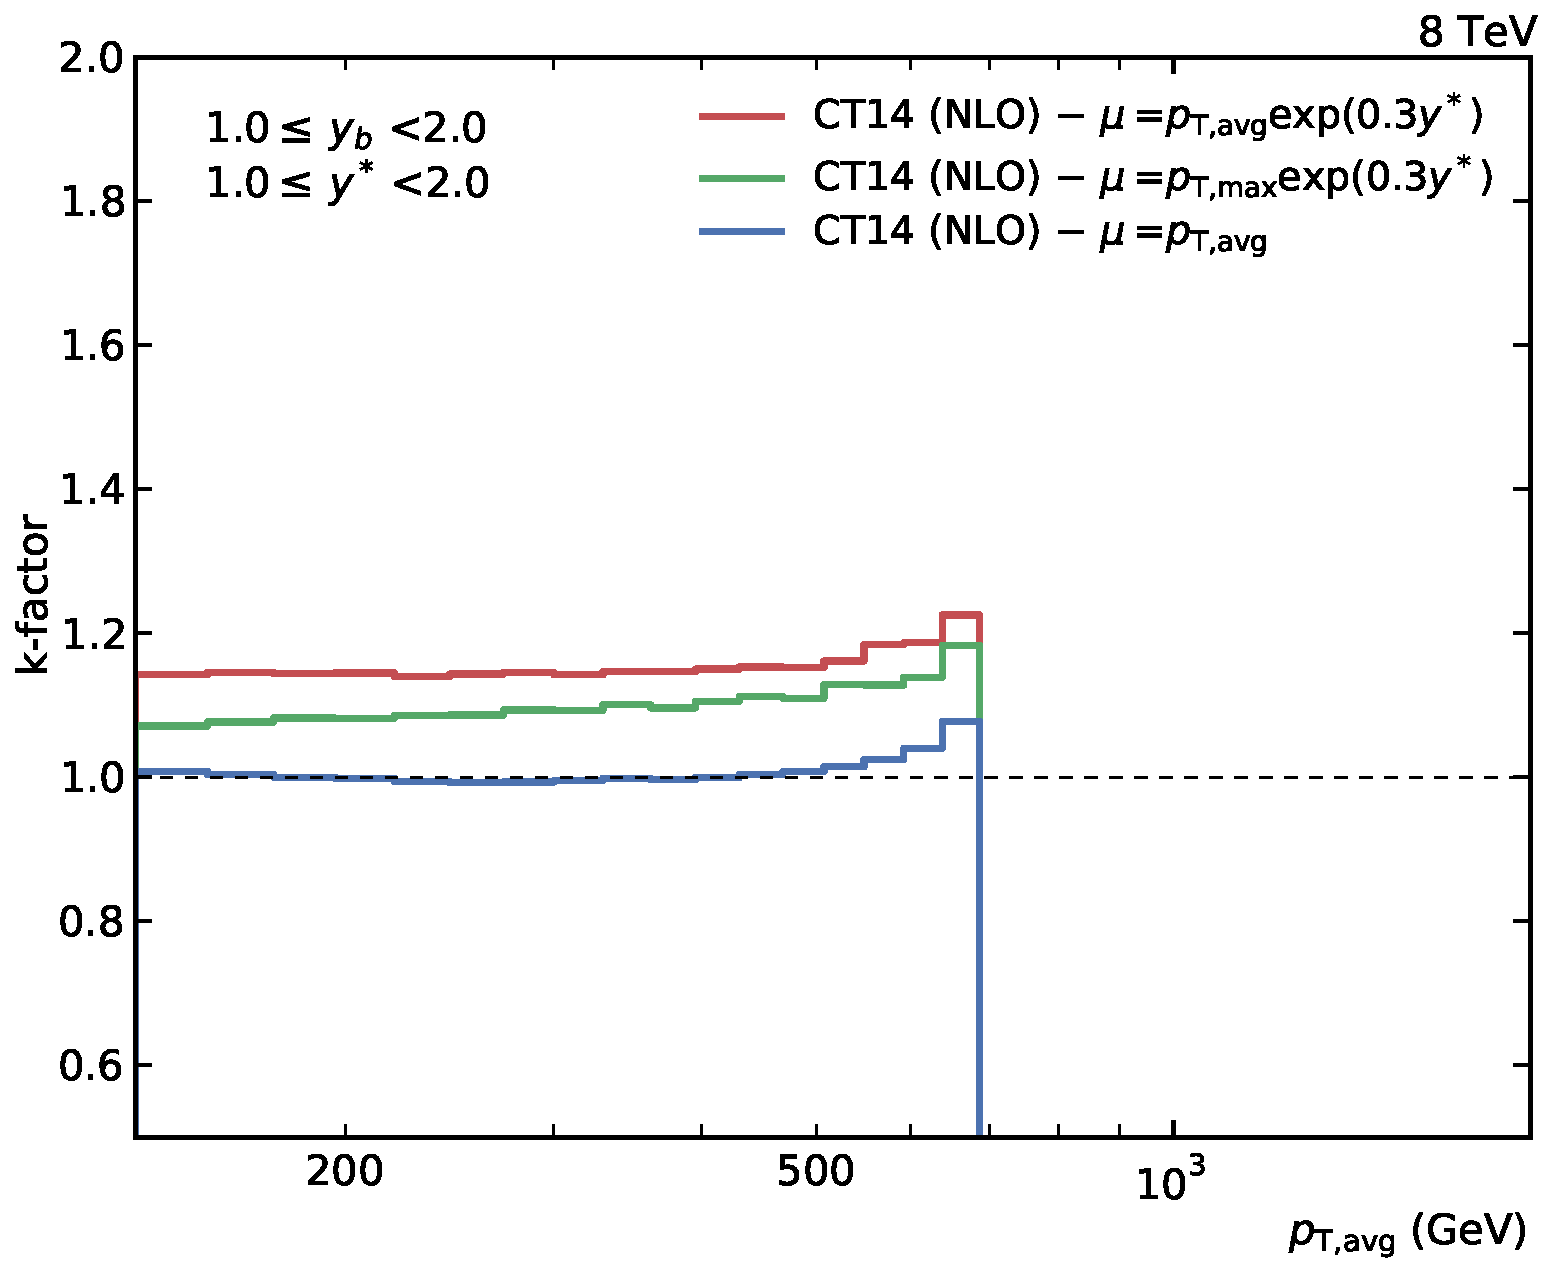
\includegraphics[width=0.45\textwidth]{figures/theory/kfactor_comp_yb1ys1.pdf}\hfill
    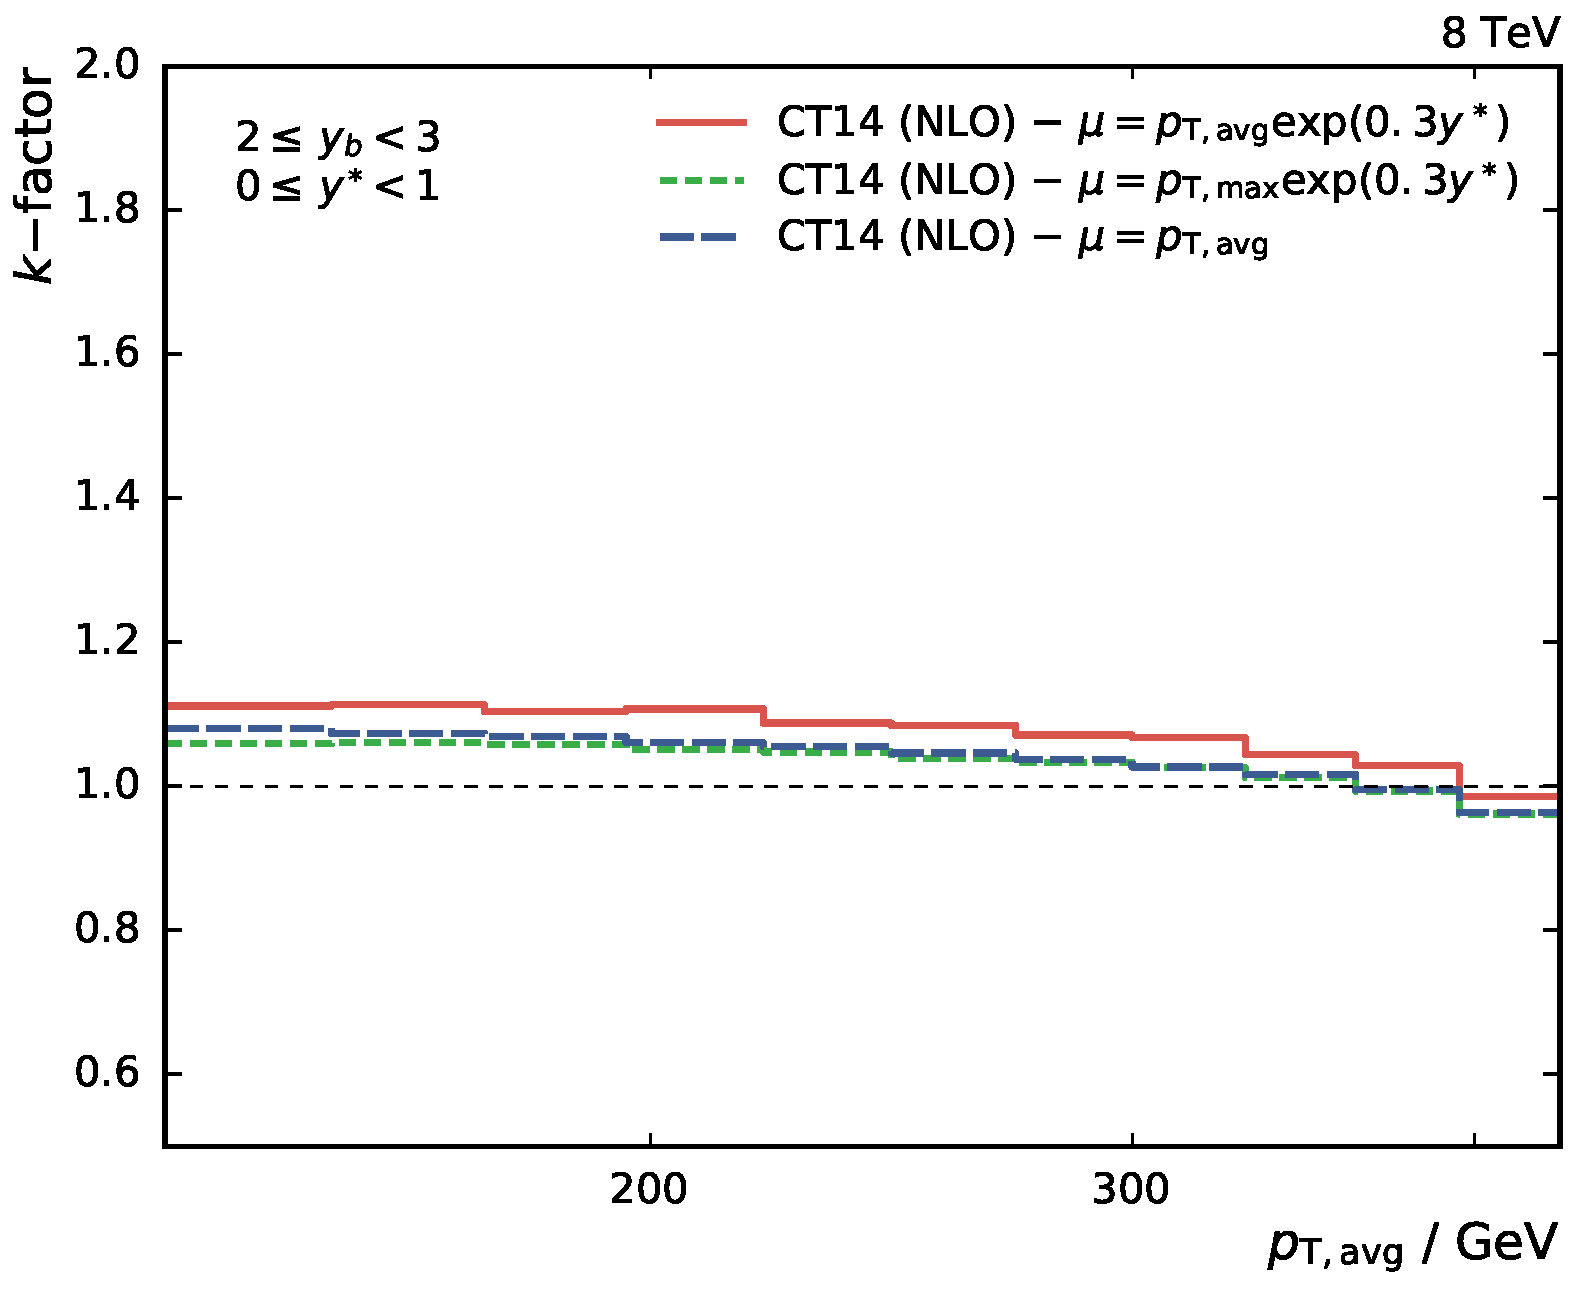
\includegraphics[width=0.45\textwidth]{figures/theory/kfactor_comp_yb2ys0.pdf}
    \caption{The $k$-factors between the NLO calculation and LO calculation
        shows the influence of the NLO correction terms. The $k$-factors for the
        calculation with \ptavg as scale choice fall below unity in case of high
        \ystar values indicating that the NLO correction is negative in this
        phasespace region.}
    \label{fig:kfactor_comp}
\end{figure}

\section{NLO Prediction with Matched Parton Showers}

Cross section calculations beyond leading order combining parton showers, MPI
and hadronization models are very complicated. Double counting of terms in the
perturbative series and the parton shower needs to be avoided. The recently
released version of Herwig includes NLO predictions with matched parton showers.
The calculation uses the MC@NLO type matching as it is implemented in the
Matchbox module~\cite{Platzer:2011bc} of Herwig. The PDFs of the MMHT 2014 NLO PDF set are accessed
using LHAPDF. For the calculation of the matrix elements, the
NJet~\cite{Badger:2012pg} library is interfaced to Herwig and the scale choice
is set to $\mu = \ptmax$. As the integration and event generation steps are
extremely time consuming the phase space was split into 12 mutually exclusive
regions binned in the transverse momentum of the leading jet and the phase space
regions were stitched together on analysis level.

\todo{add and describe figure with results.}

\section{Non-Perturbative Corrections}
\label{sec:np_factors}

The perturbative QCD calculations of \NLOJETPP give a cross section at NLO
parton level. These so-called fixed-order pQCD calculations cannot directly
compared to the unfolded data, as they do not include additional soft QCD
effects. While a part of these effects is absorbed by the applied jet-algorithm,
they still must be estimated and accounted for in comparisons of fixed-order
calculations to data.

The effects of these soft effects are estimated using Monte Carlo event
generators which are able to simulate those. The usual approach consists of
calculating the cross section including effects from multi-parton interactions
(MPI) and hadronization. The non-perturbative (NP) correction $c_k^\mathrm{NP}$
obtained with a MC event generator $k$ is defined as the ratio between the
nominal cross section including the effects and a cross section calculation
neglection those, see Eq.~\ref{eq:np_definition}. The superscript in the
equation indicates the applied steps in the simulation, the parton shower (PS),
the multi parton interaction model (MPI) and the hadronization (HAD).The
correction is then applied as a bin-by-bin correction factor to the NLO cross
section.

\begin{equation}
    c_{k}^{\mathrm{NP}} = \frac{\sigma^{\mathrm{PS+HAD+MPI}}}{\sigma^{\mathrm{PS}}}
    \label{eq:np_definition}
\end{equation}

The NP corrections have been calculated using two Monte Carlo
event generators using the newest available tunes within CMS. Herwig++ is used
with the tune UE-EE-5C and Pythia 8 with the tune CUETP8M1. The ratio is fitted
using a power-law function, see Eq.~\ref{fcn:np_fit}.

\begin{equation}
  f(\ptavg) = a \cdot \ptavg^b + c
  \label{fcn:np_fit}
\end{equation}

Since the correction factors obtained from Herwig++ and Pythia8 are quite
different in the low-\pt region, an uncertainty was assigned to the correction
factor. The correction factors are determined from the average of the factors
obtained from the Pythia 8 and Herwig++ predictions.

\begin{equation*}
    c^\mathrm{NP} = \frac{c_{\mathrm{P8}}^{\mathrm{NP}} + c_{\mathrm{HW++}}^{\mathrm{NP}}}{2}
\end{equation*}

The uncertainty quoted for the NP correction factors is half the difference
between the two corrections factors.

Fig.~\ref{fig:np_factors} shows the resulting correction factors and the
corresponding uncertainty.  The corrections are of the size of 10\% to 15\% at
100 \si{GeV} and get smaller at higher values of \ptavg. While the correction
decreases for higher transverse momenta, it does not approach unity especially
in the bins containing jets with high rapidities. 

\begin{figure}[htp]
    \centering
    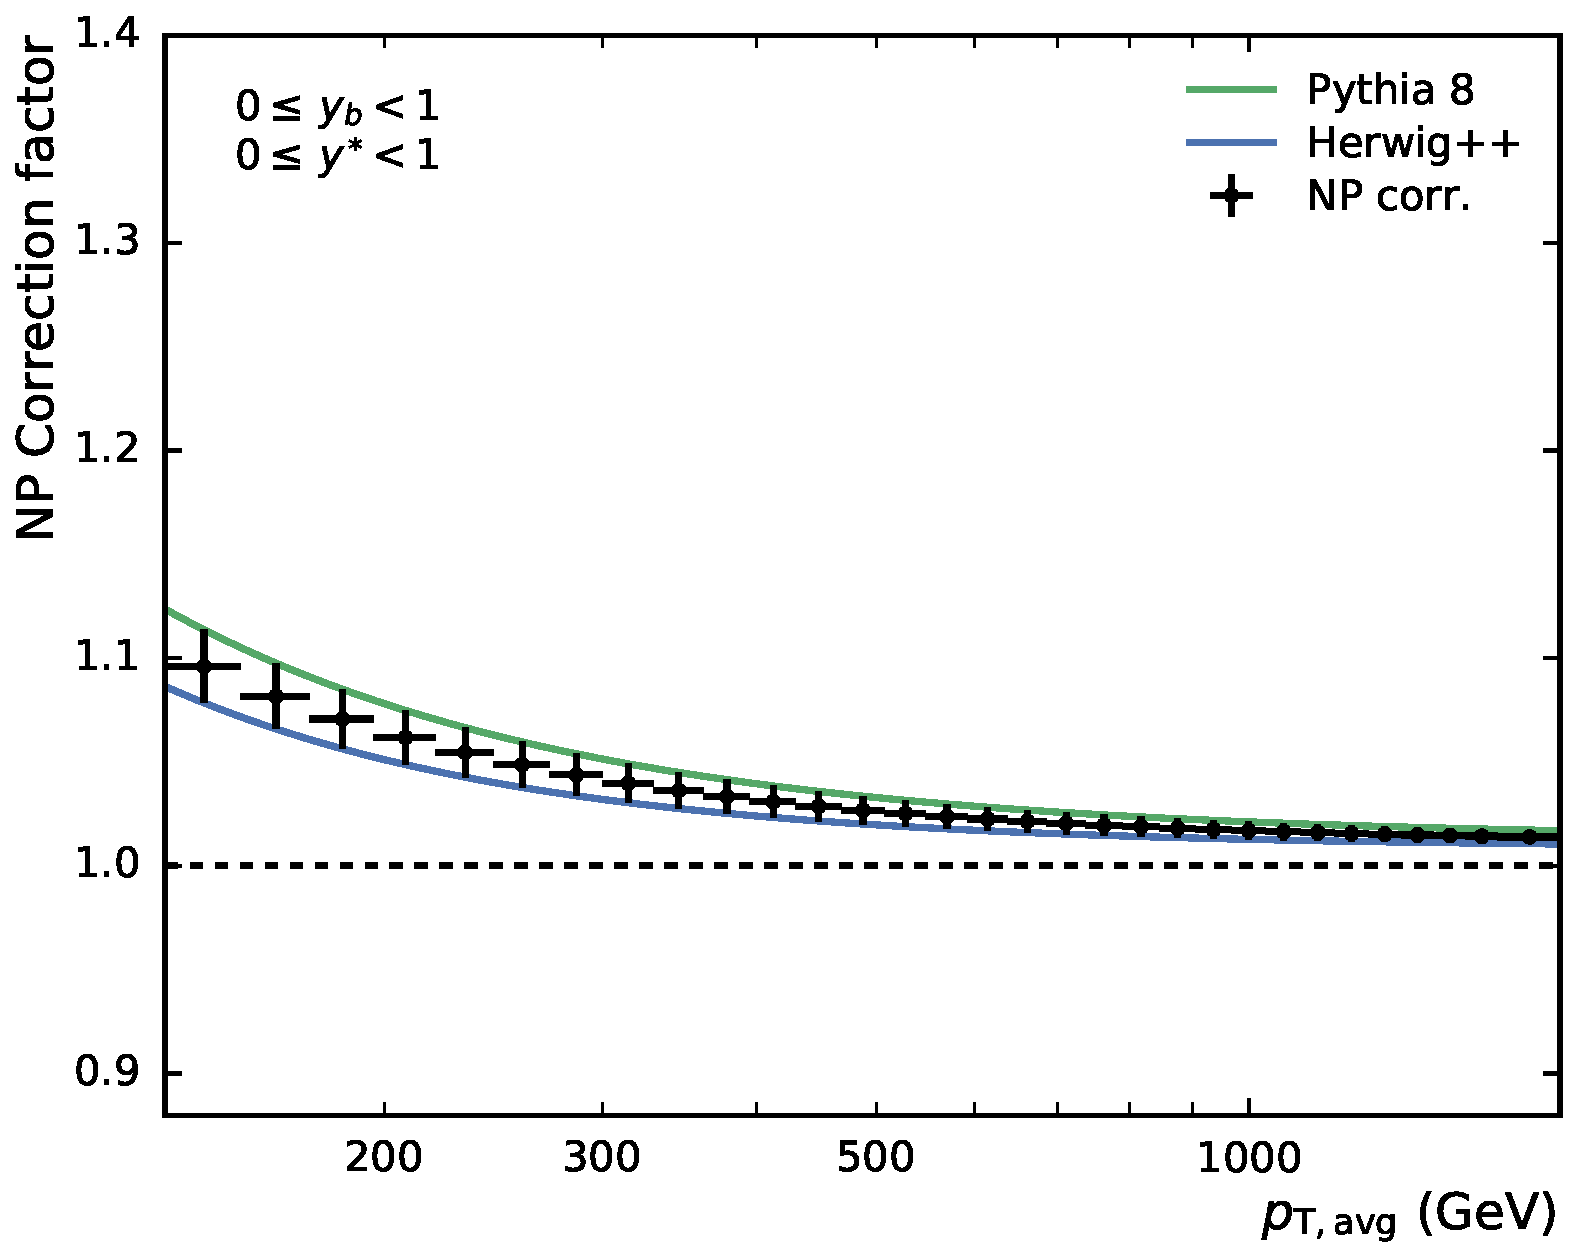
\includegraphics[width=0.45\textwidth]{figures/theory/np_factors_calc_yb0ys0.pdf}\hfill
    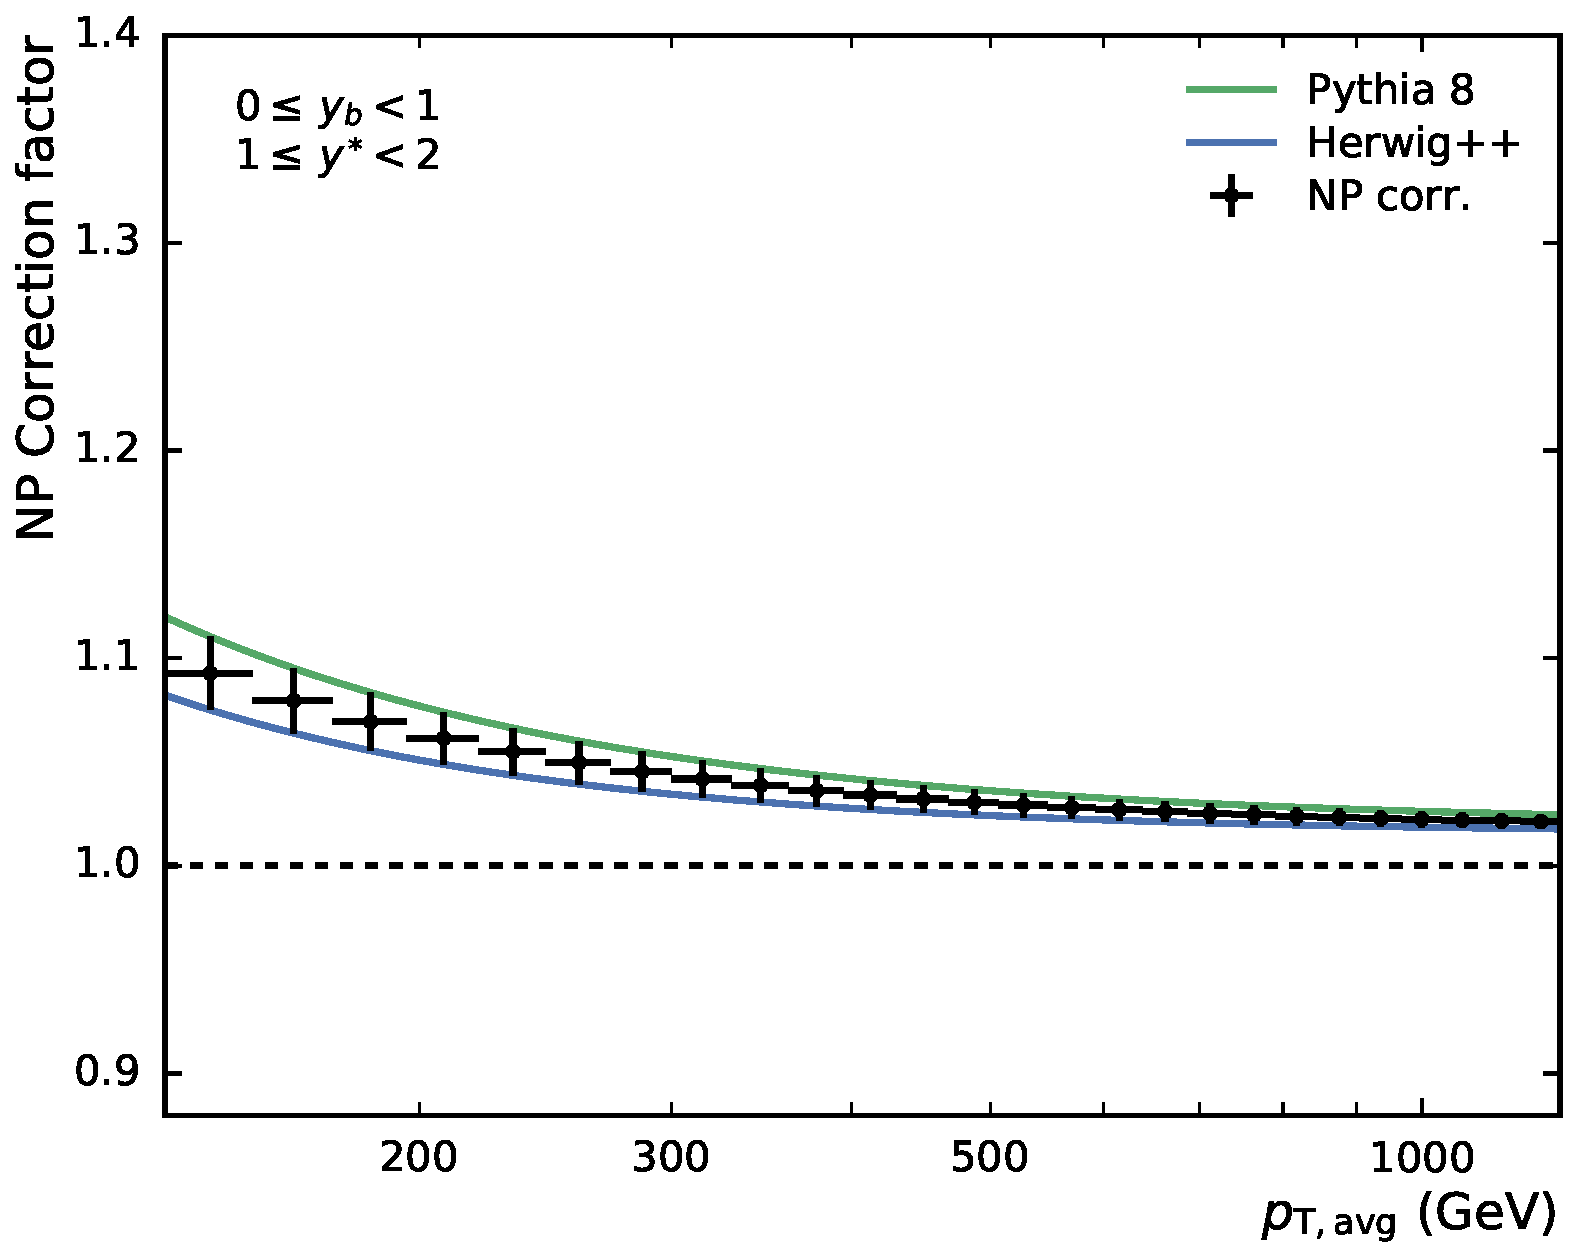
\includegraphics[width=0.45\textwidth]{figures/theory/np_factors_calc_yb0ys1.pdf}
    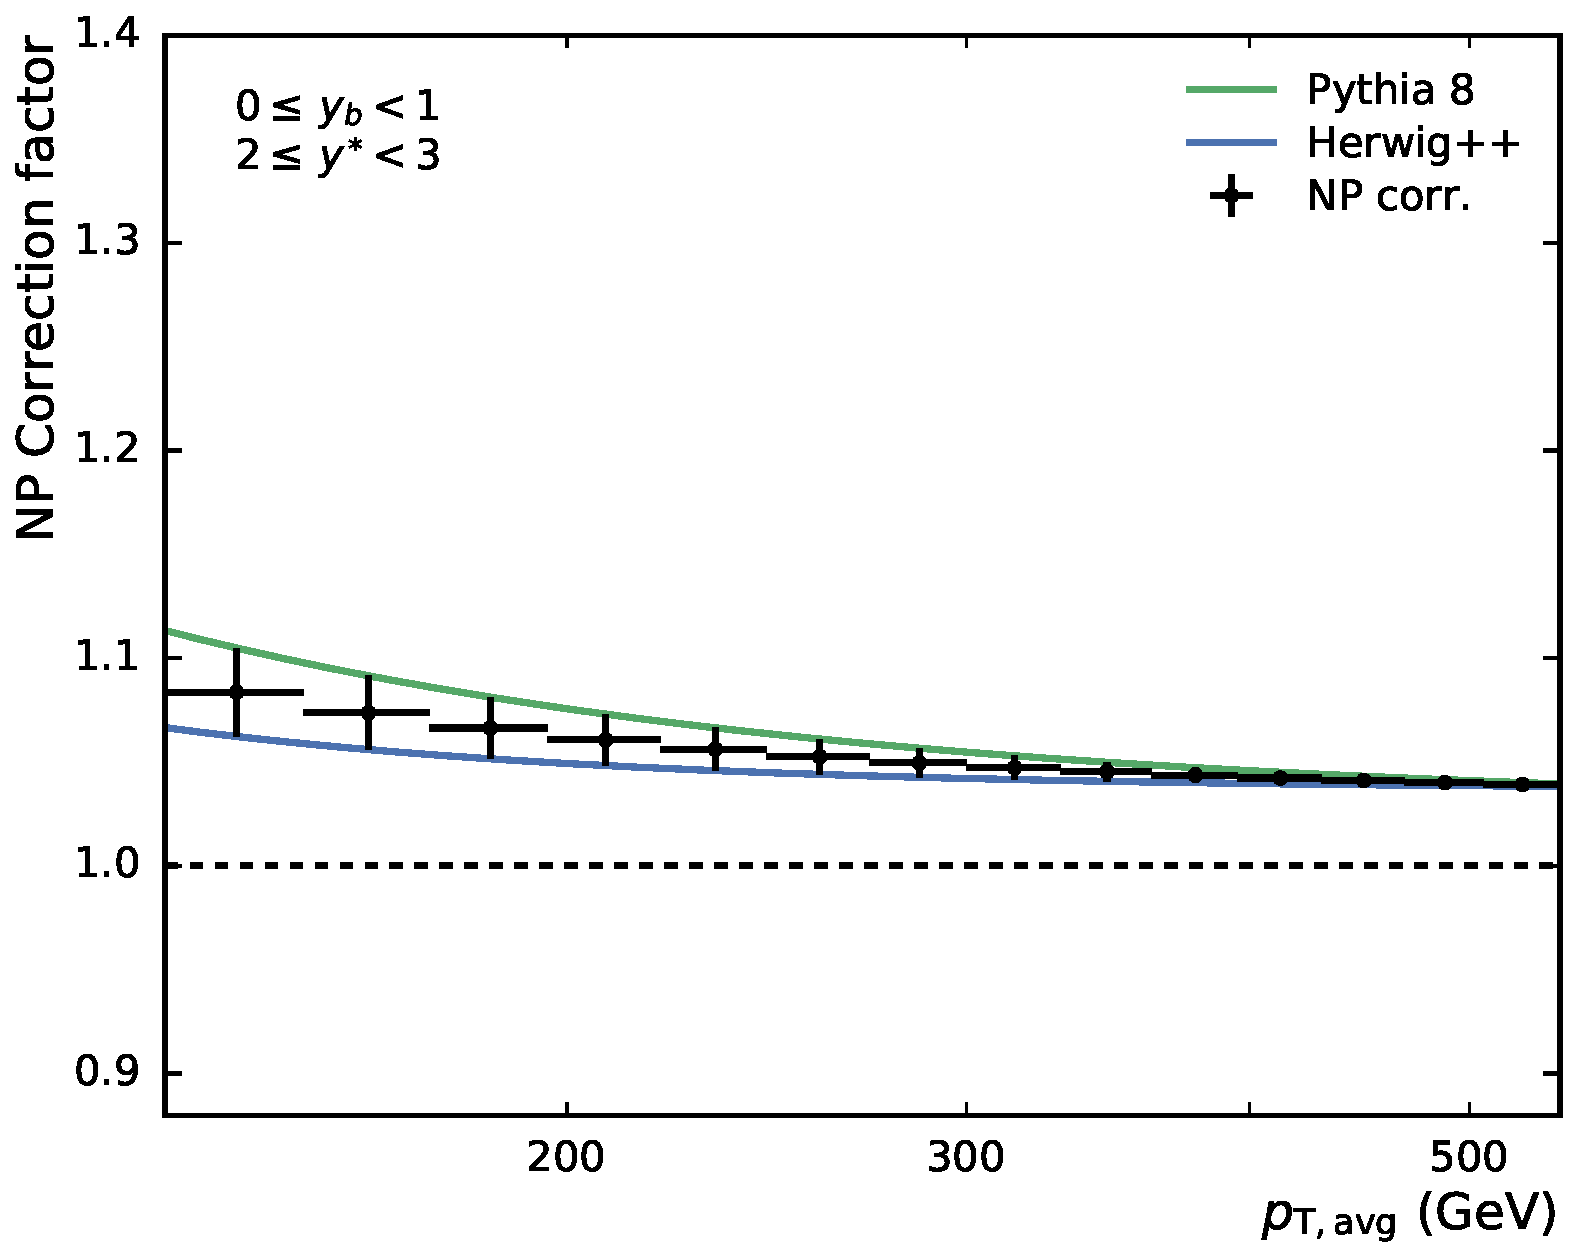
\includegraphics[width=0.45\textwidth]{figures/theory/np_factors_calc_yb0ys2.pdf}\hfill
    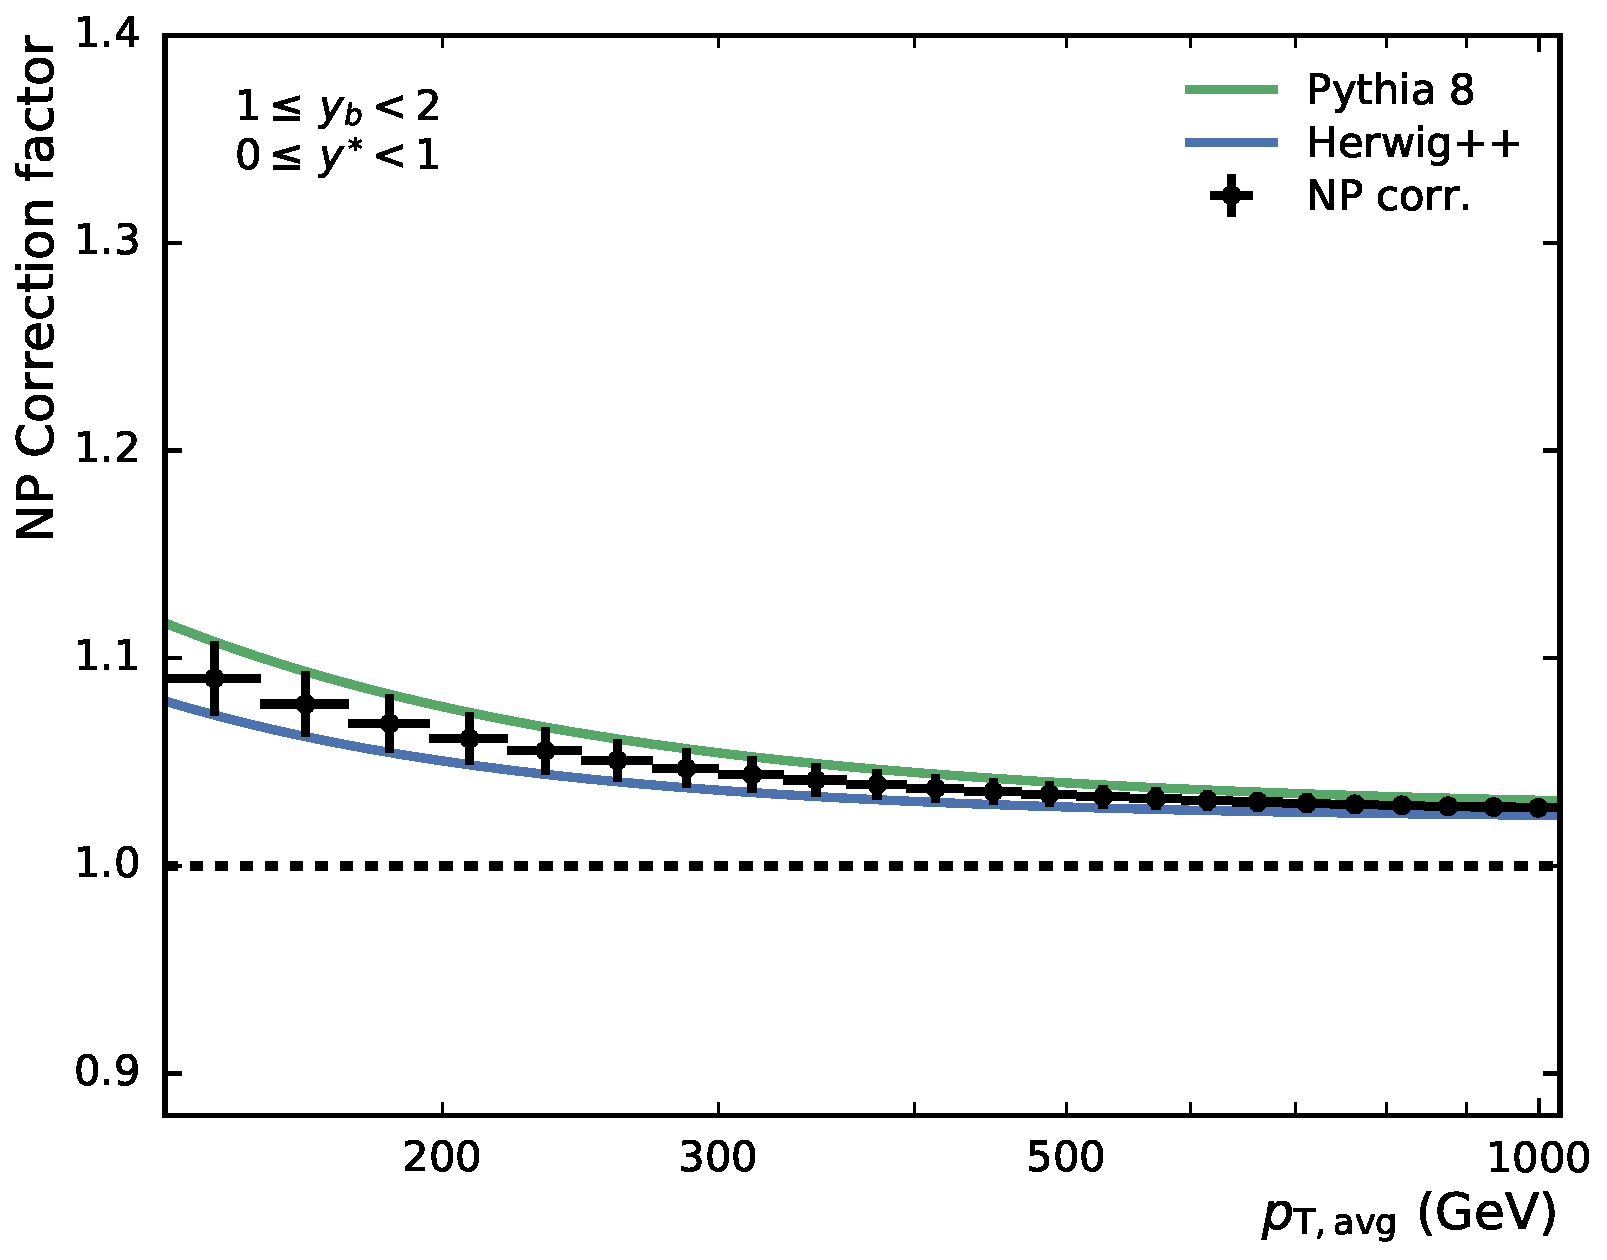
\includegraphics[width=0.45\textwidth]{figures/theory/np_factors_calc_yb1ys0.pdf}
    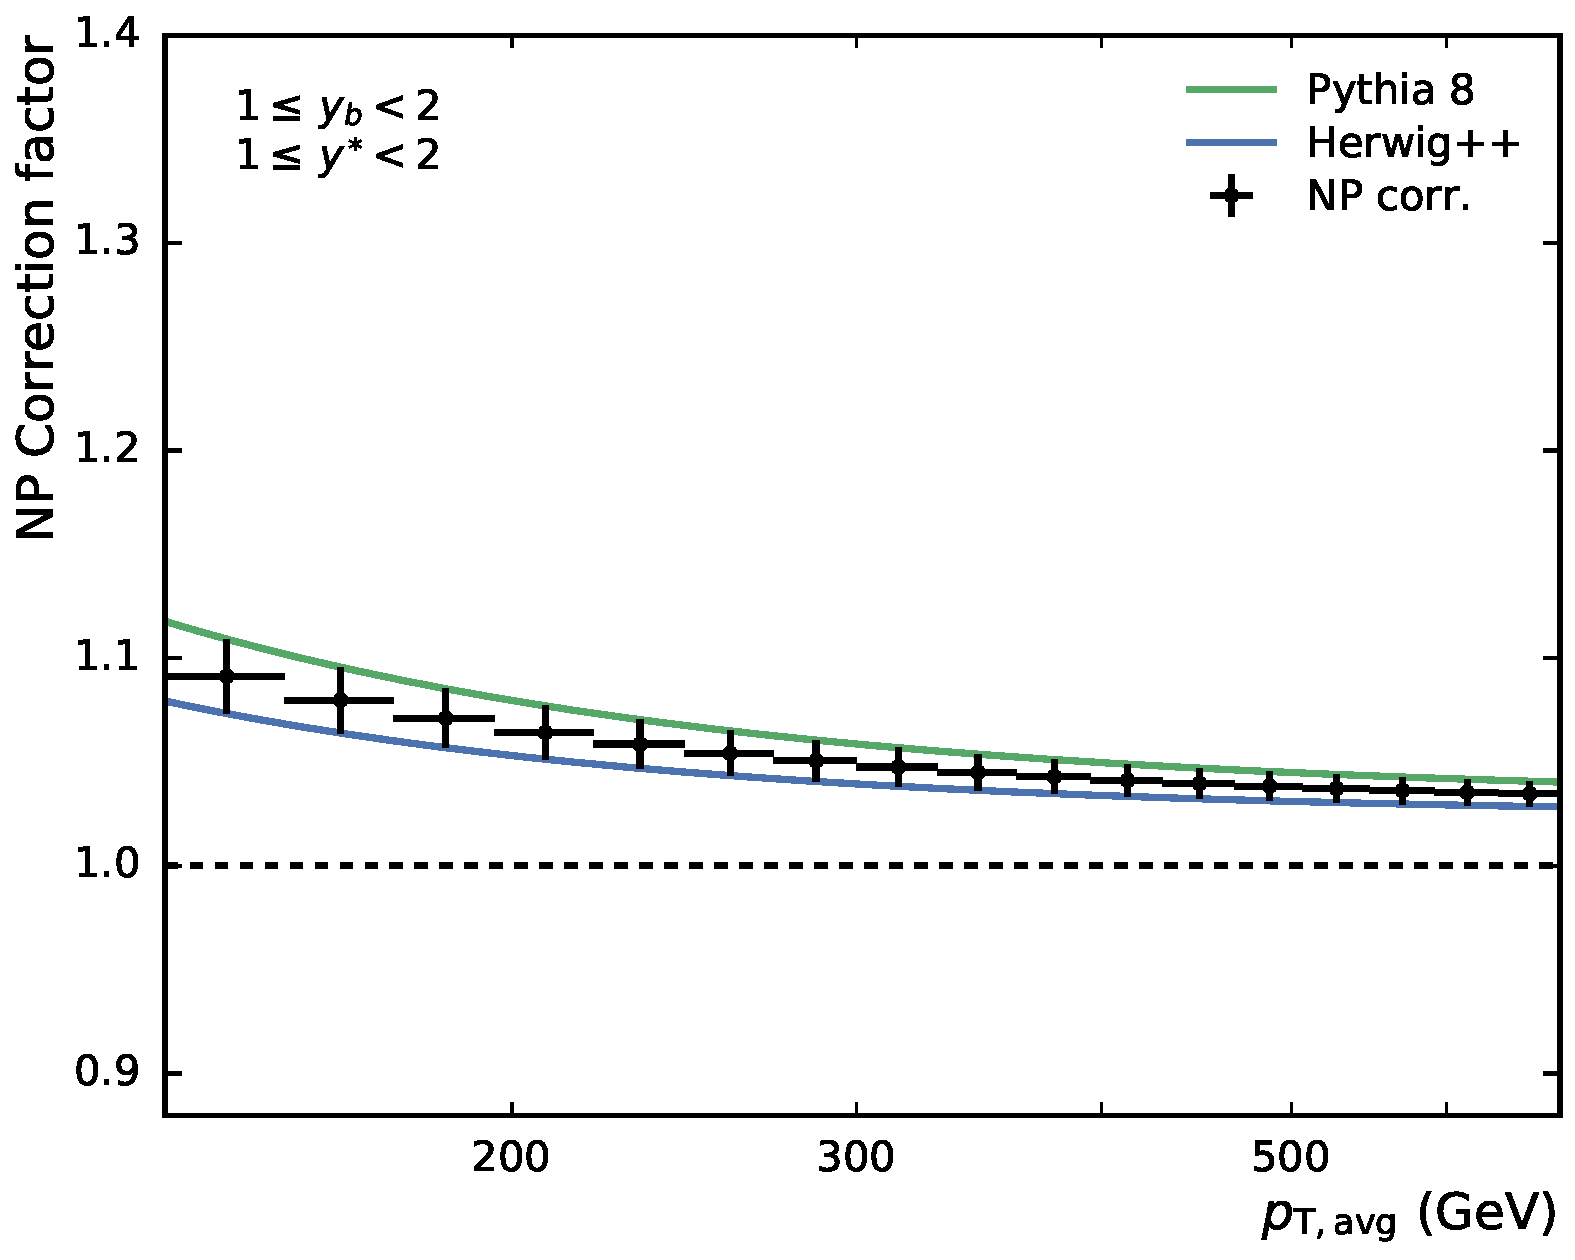
\includegraphics[width=0.45\textwidth]{figures/theory/np_factors_calc_yb1ys1.pdf}\hfill
    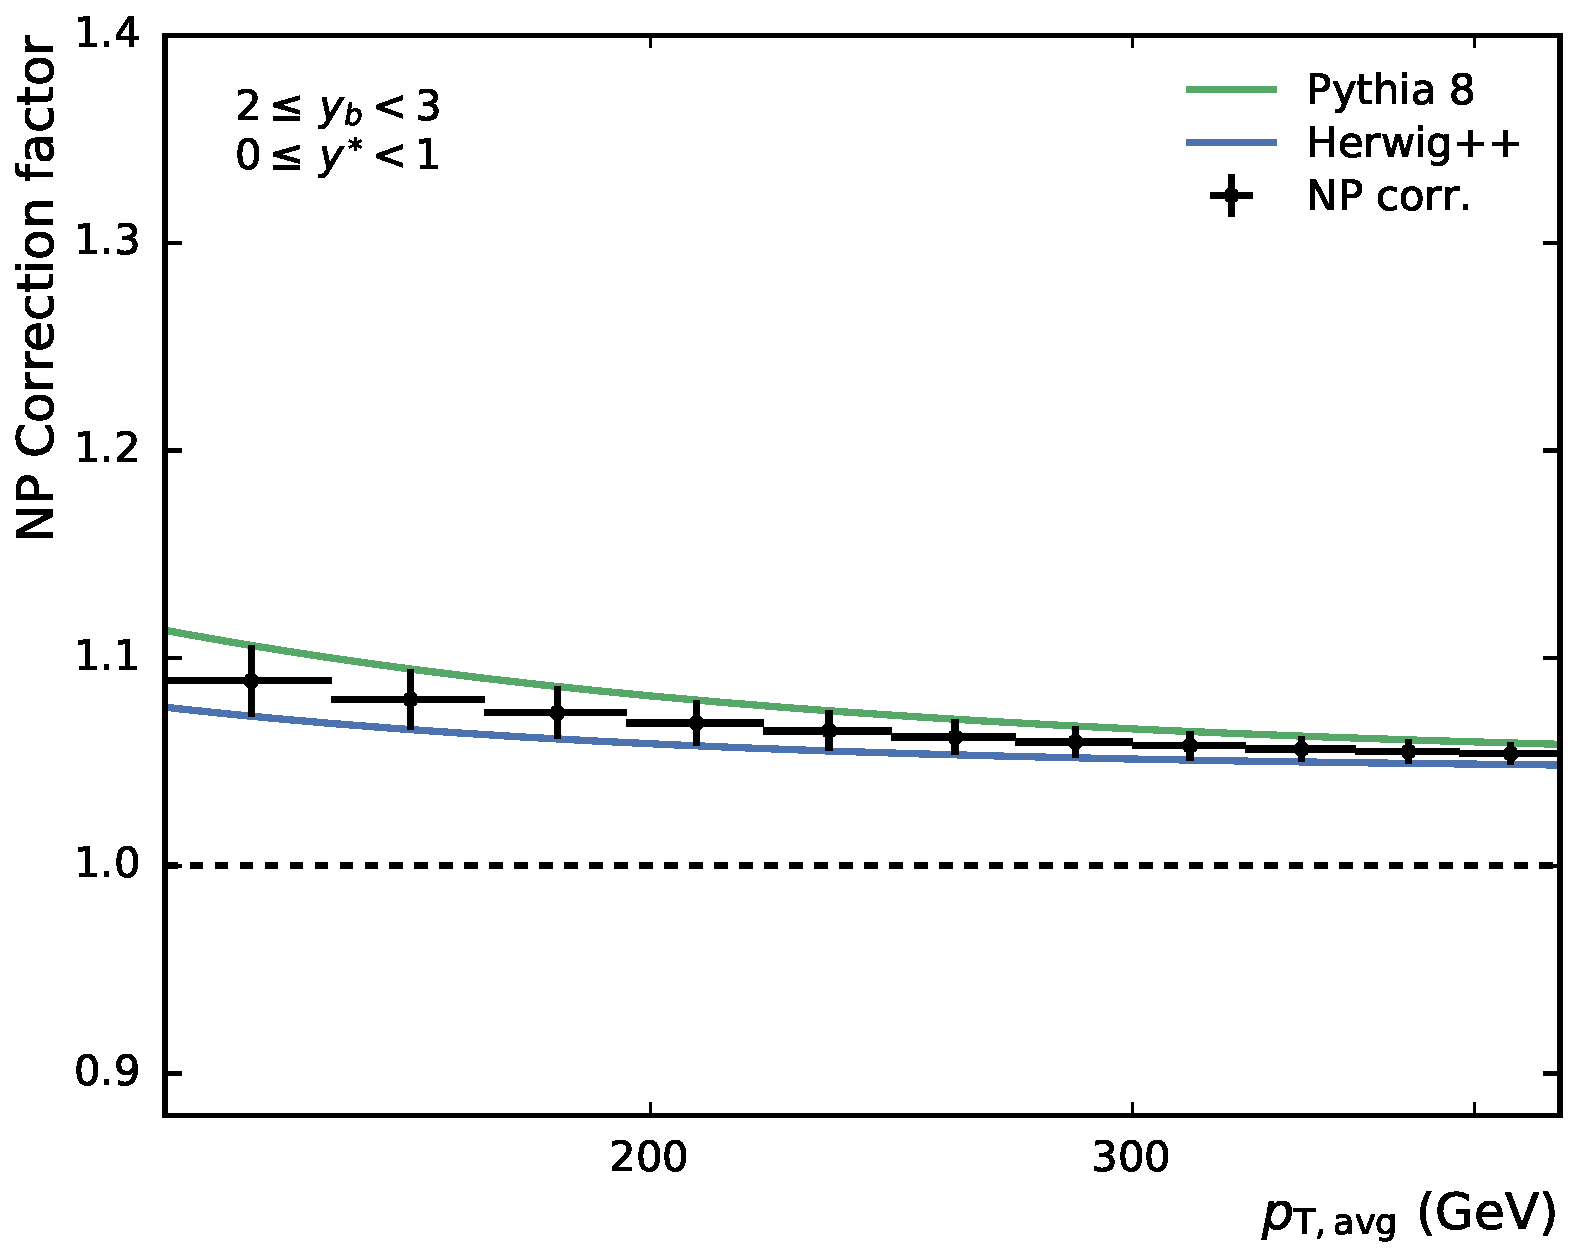
\includegraphics[width=0.45\textwidth]{figures/theory/np_factors_calc_yb2ys0.pdf}
    \caption{The non-perturbative correction is derived using a MC event
        generator by calculating the diferences by including hadronization and
        MPI in the simulation. The green line shows the correction of Pythia 8,
        the blue line the correction of Herwig++. The average of both gives the
        central correction and the envelope the uncertainty on the correction.}
    \label{fig:np_factors}
\end{figure}

\section{Theory Uncertainties}

Multiple sources of uncertainty limit the precision of the NLO cross section
calculation. In this section, the derivation of the scale, PDF and NP
uncertainties is described. 

A comparison of all studied theoretical uncertainties is shown in
Fig.~\ref{fig:theo_uncertainties}. The scale uncertainty is the dominant source
of uncertainty in the low-\pt region and is of the size of 5\% to 10\% most of
the time. For increasing transverse momenta of the dijet system, the PDF
uncertainties become the dominant uncertainties. The size ranges from 5\% in the
low-\pt region up to 50\% for highest \pt. The uncertainty afflicted to
non-perturbative corrections is only sizeable for lower \pt and less than 5\%
all the time.

As the cross section calculation is performed using \fastNLO interfaced to
\NLOJETPP, multiple independent calculations can be merged to increase the
statistical precision. The statistical uncertainty is estimated by calculating
the uncertainty on the arithmetic mean of the cross section of all fastNLO
tables.  The statistical uncertainty is found to be smaller than 0.5\% in all
bins, in most of the bins even smaller than 0.1\%. Therefore the statistical
uncertainty is neglected in all further comparisons.

\subsection{Scale uncertainties}
\label{sec:scale_uncertainties}

As discussed in Sec.~\ref{sec:scale_coice}, one has to choose a factorization
and renormalization scale for a perturbative cross section calculation. Due to
the truncated perturbative series, a scale dependence remains. The effects of
neglected higher-order contributions are collected in a source of uncertainty.

There is a common approach in estimating the influence of the scale on the cross
section~\cite{Banfi:2010xy}. The cross section calculation is performed using
multiple scale choices and the differences compared to the cross section
obtained using the central scale choice are translated into an uncertainty,
called scale uncertainty. The variations are applied as multiplicative factors
to the central choice in the following six combinations: $(\mur, \muf) =
(\sfrac{1}{2}, \sfrac{1}{2}), (\sfrac{1}{2}, 1), (1, \sfrac{1}{2}), (1, 2), (2,
1)$ and $(2, 2)$. The uncertainty on a quantity $X$, \eg the cross section, is
the envelope of the maximum deviation in the upwards and downwards direction
while $X^0$ depicts the value of the quantity with the central scale factors and
$n$ the number of variations.

\begin{align*}
    \Delta X^+ &= \max_{i}^{n} \left[ X^i - X^0, 0 \right]\\
    \Delta X^- &= \max_{i}^{n} \left[ X^0 - X^i, 0 \right]
\end{align*}


Fig.~\ref{fig:theo_uncertainties} shows the relative size of the scale
uncertainty for each bin of the measurement and the discussed scale choices. The
scale uncertainty is in most cases very reasonable and of the size of 5\% to
10\%. However, when using the scale choice $\mu=\ptavg$, the bin with the large
rapidity separation exhibits a large increase of the uncertainty up to 40\%
which is undesired.

\begin{figure}[htp]
    \centering
    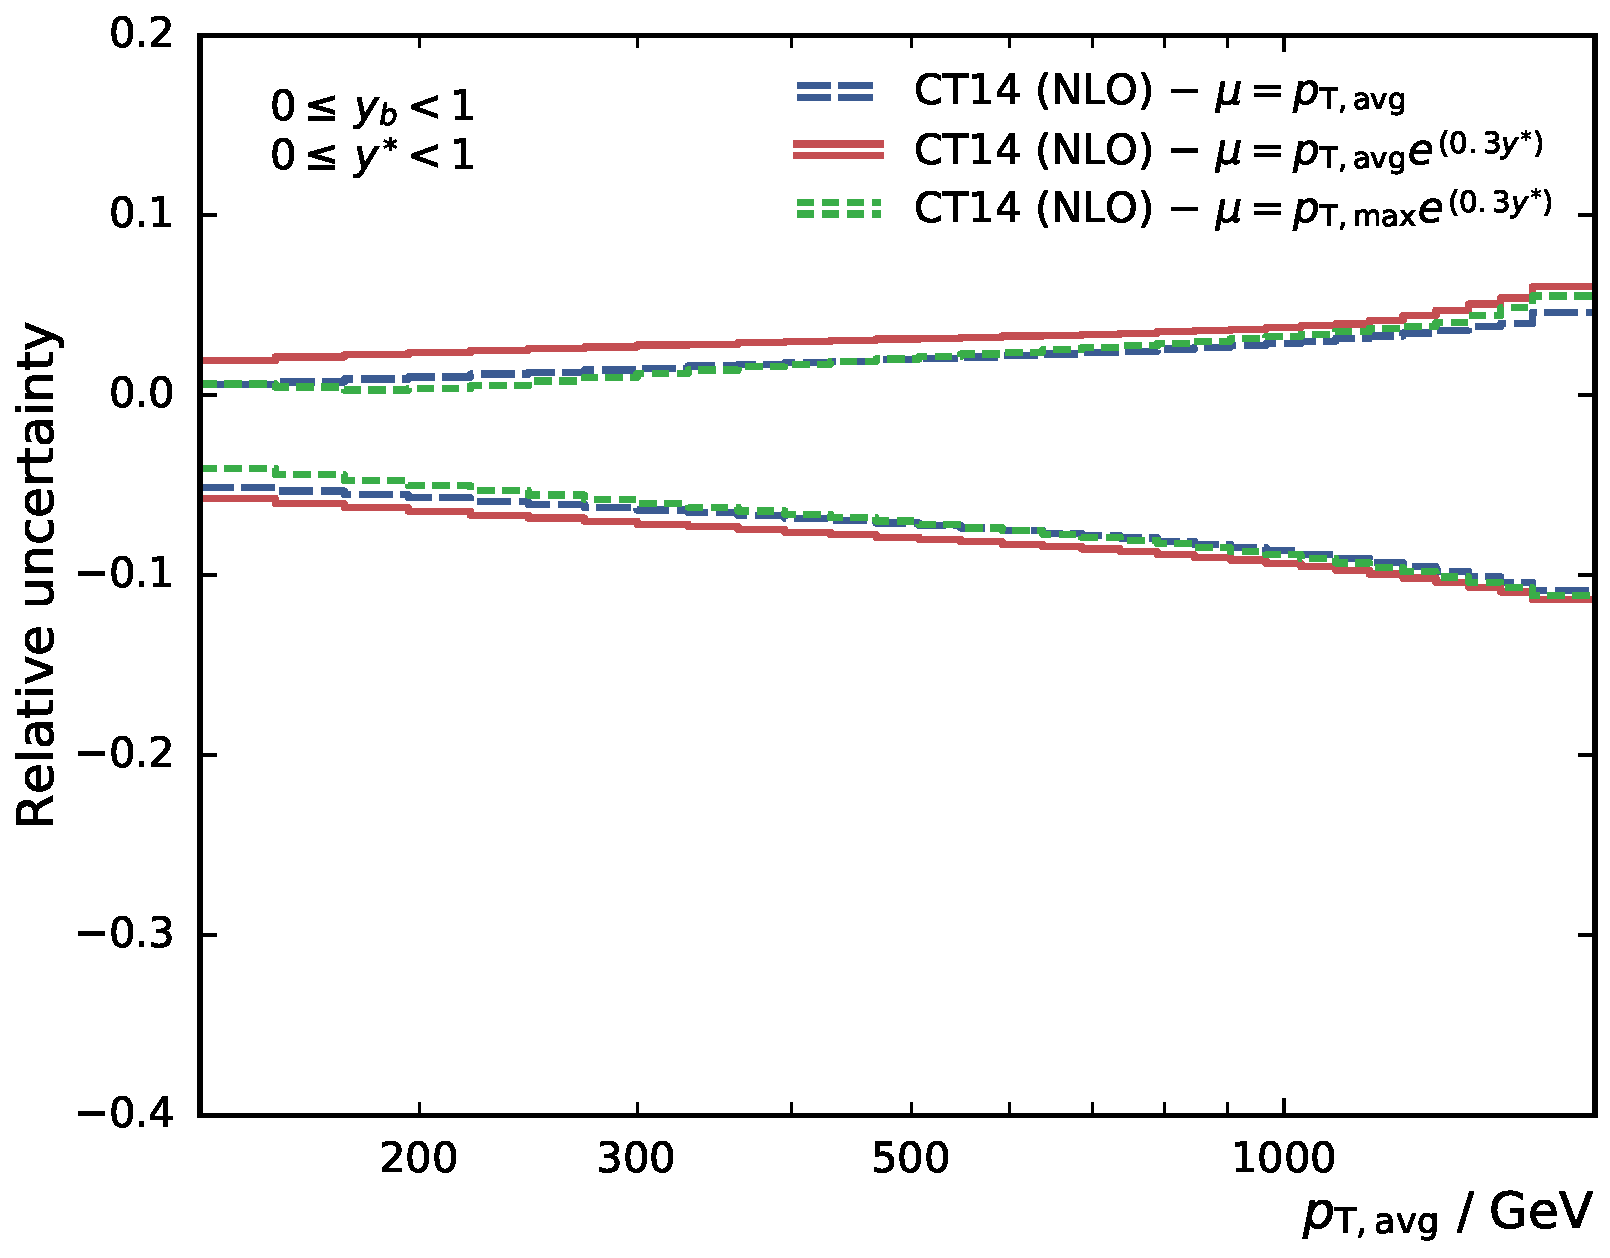
\includegraphics[width=0.45\textwidth]{figures/theory/scale_uncert_comp_yb0ys0.pdf}\hfill
    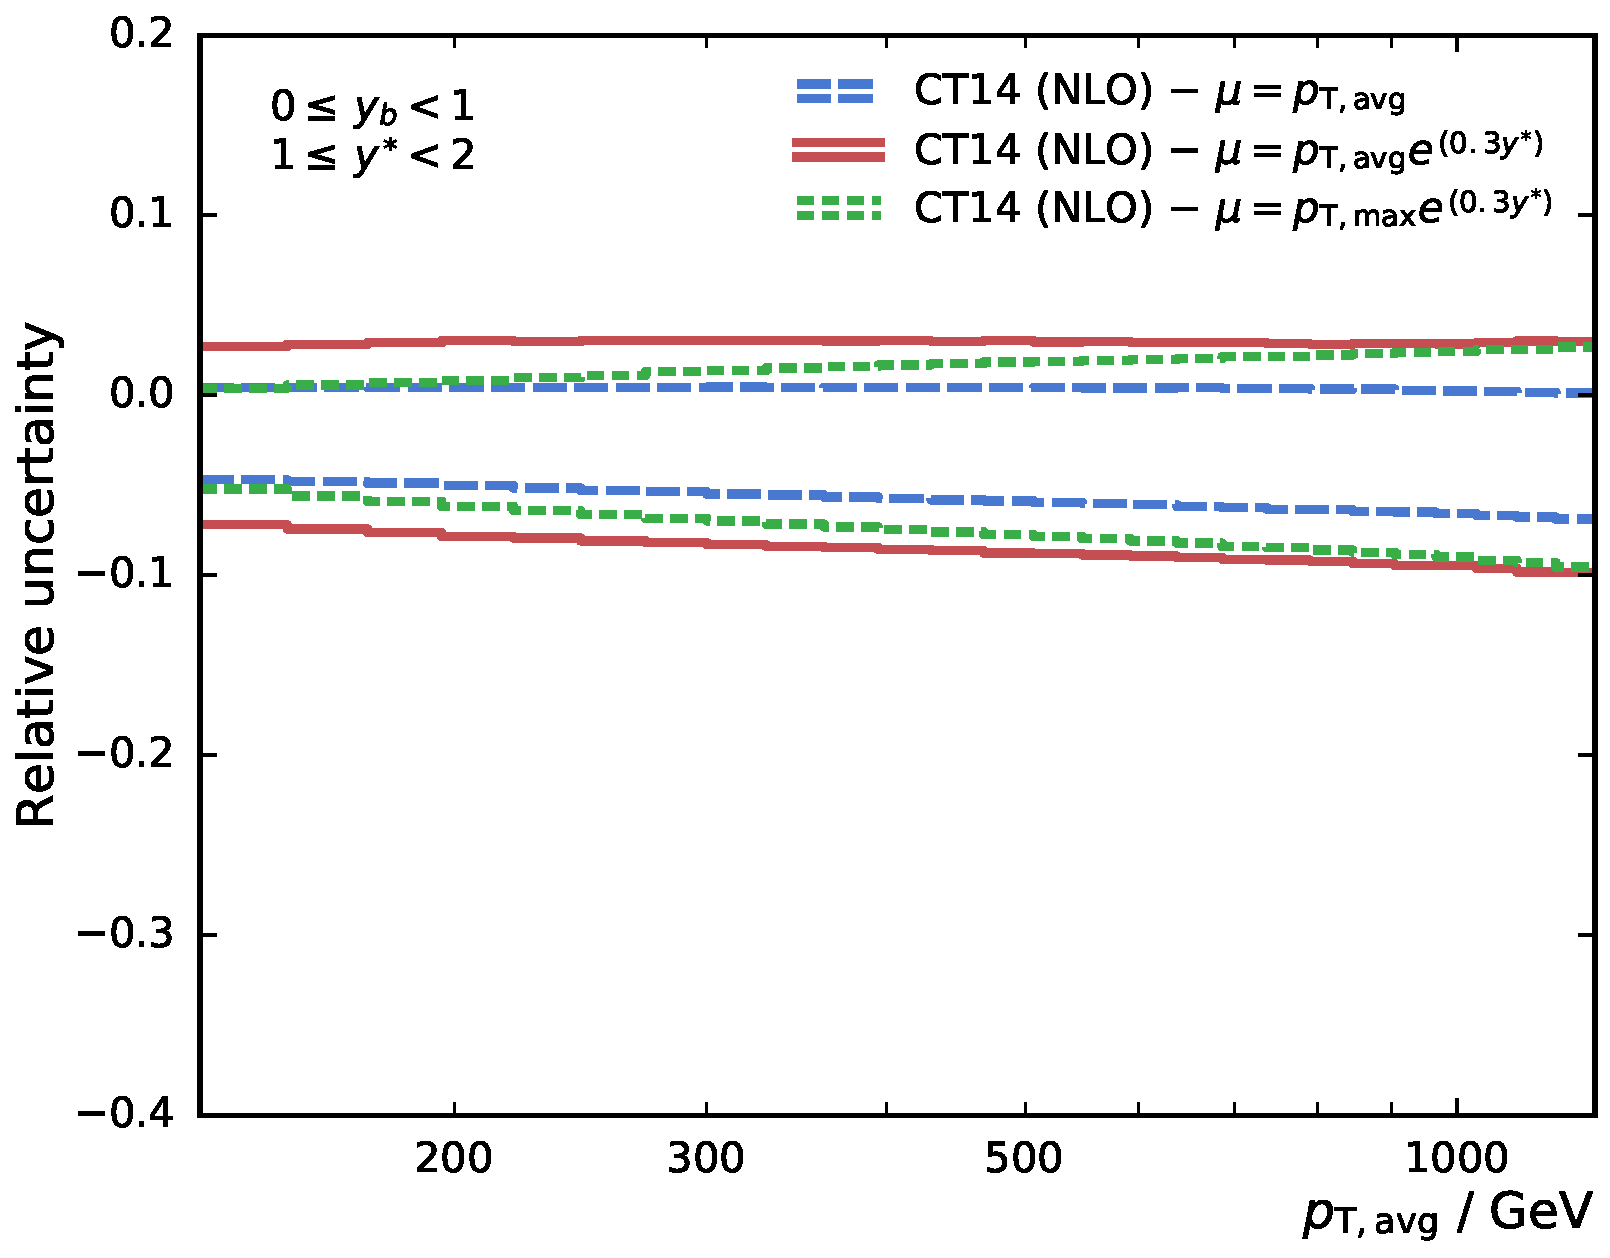
\includegraphics[width=0.45\textwidth]{figures/theory/scale_uncert_comp_yb0ys1.pdf}
    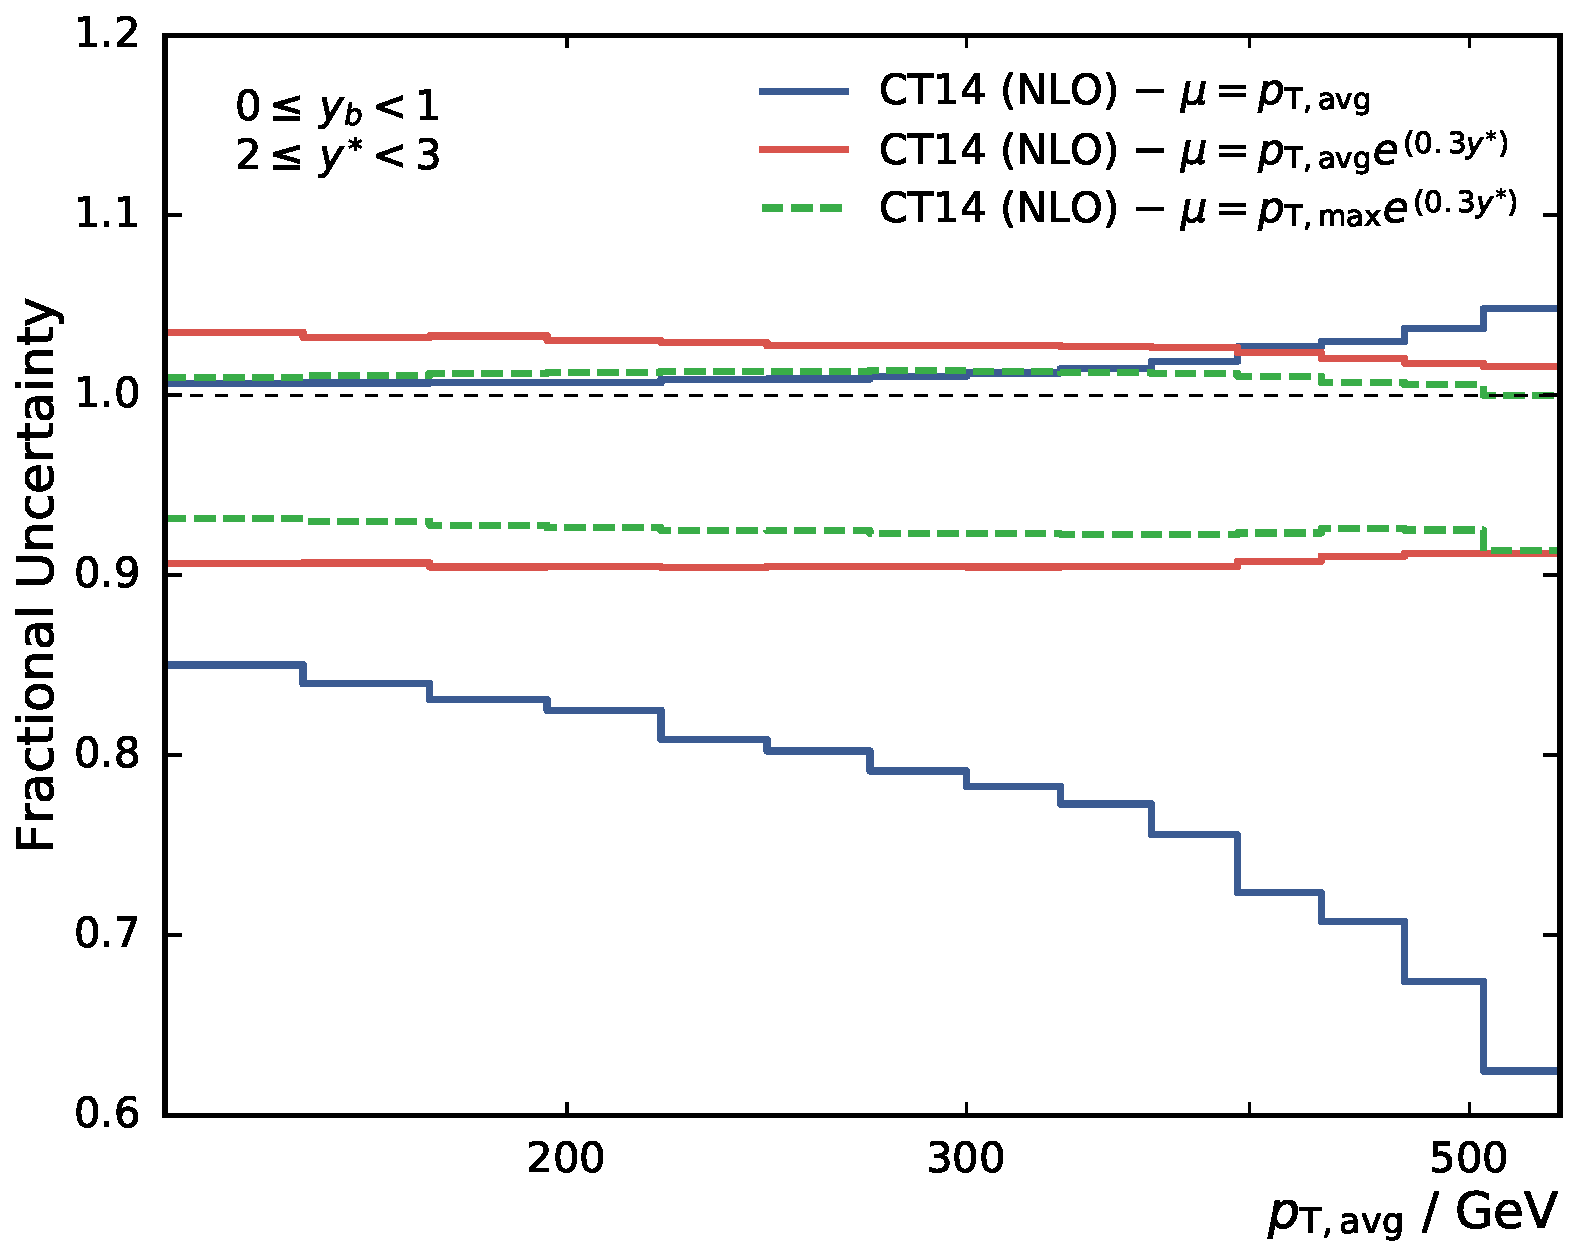
\includegraphics[width=0.45\textwidth]{figures/theory/scale_uncert_comp_yb0ys2.pdf}\hfill
    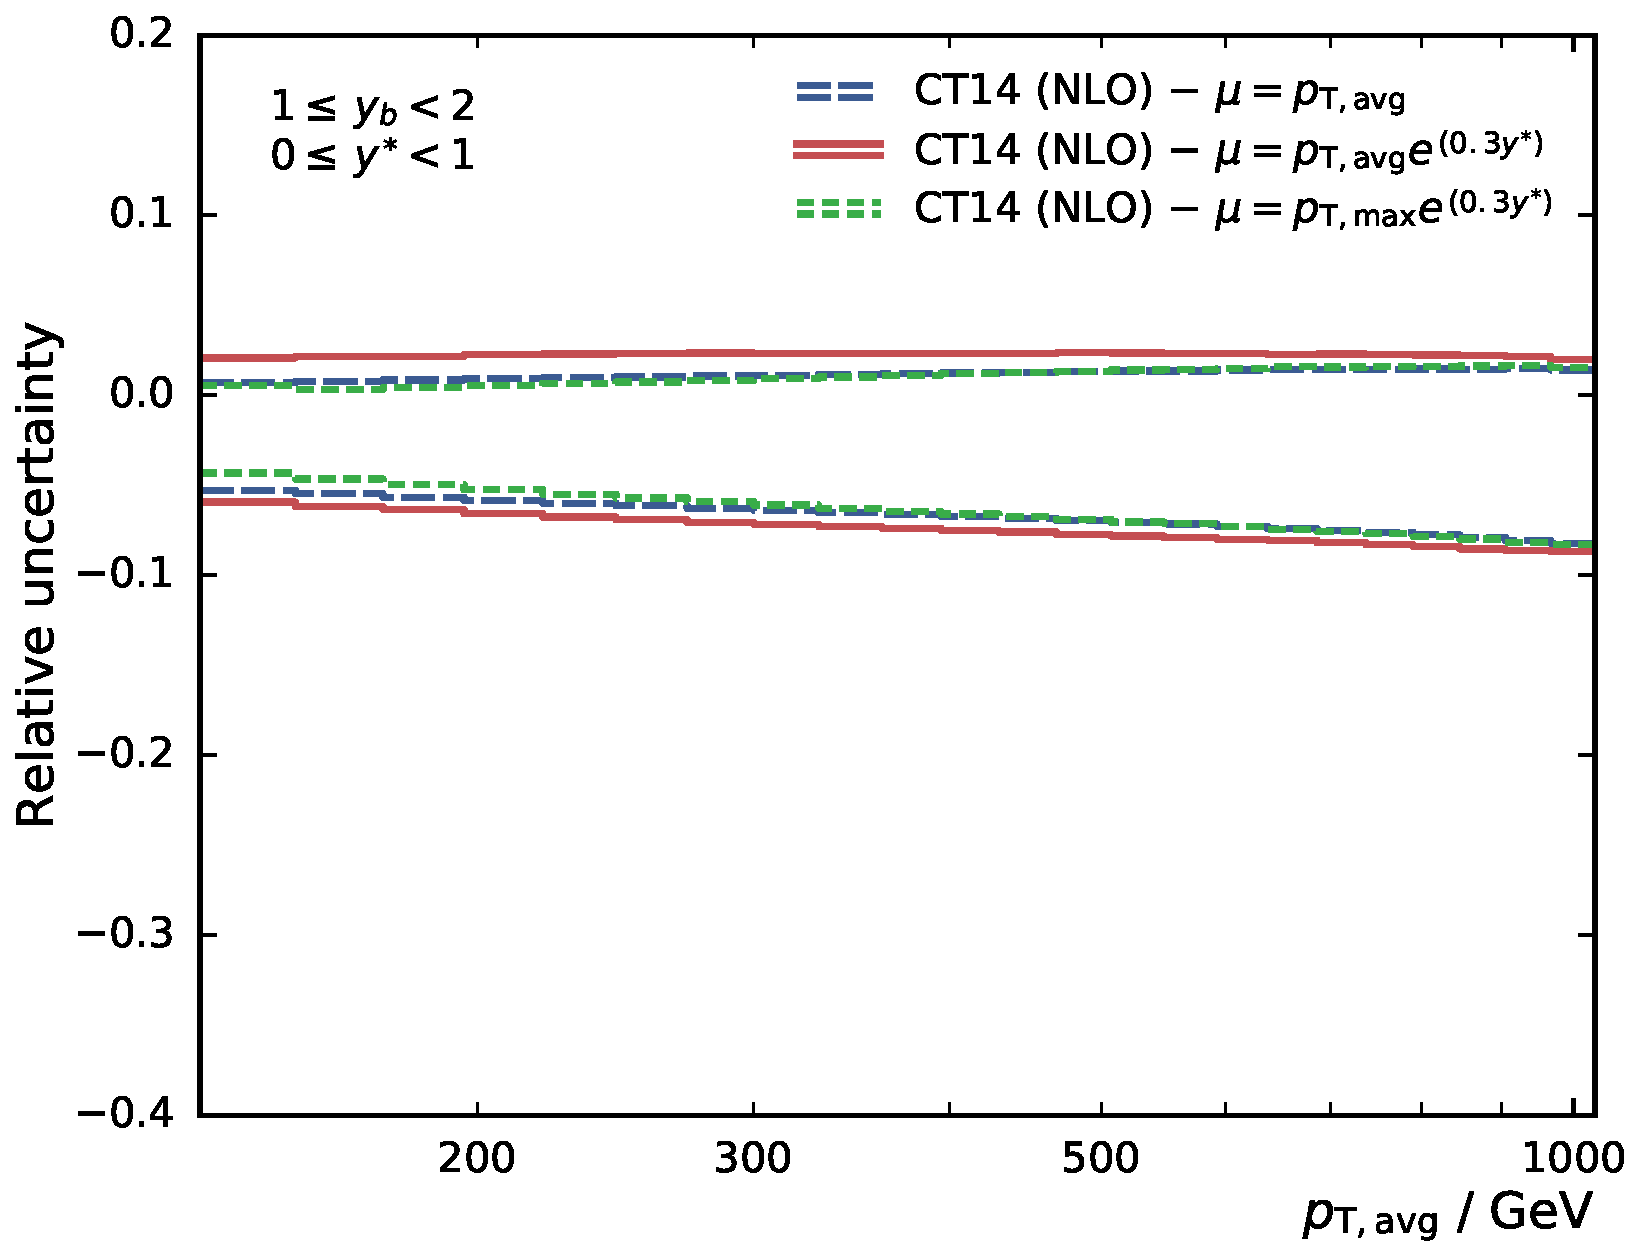
\includegraphics[width=0.45\textwidth]{figures/theory/scale_uncert_comp_yb1ys0.pdf}
    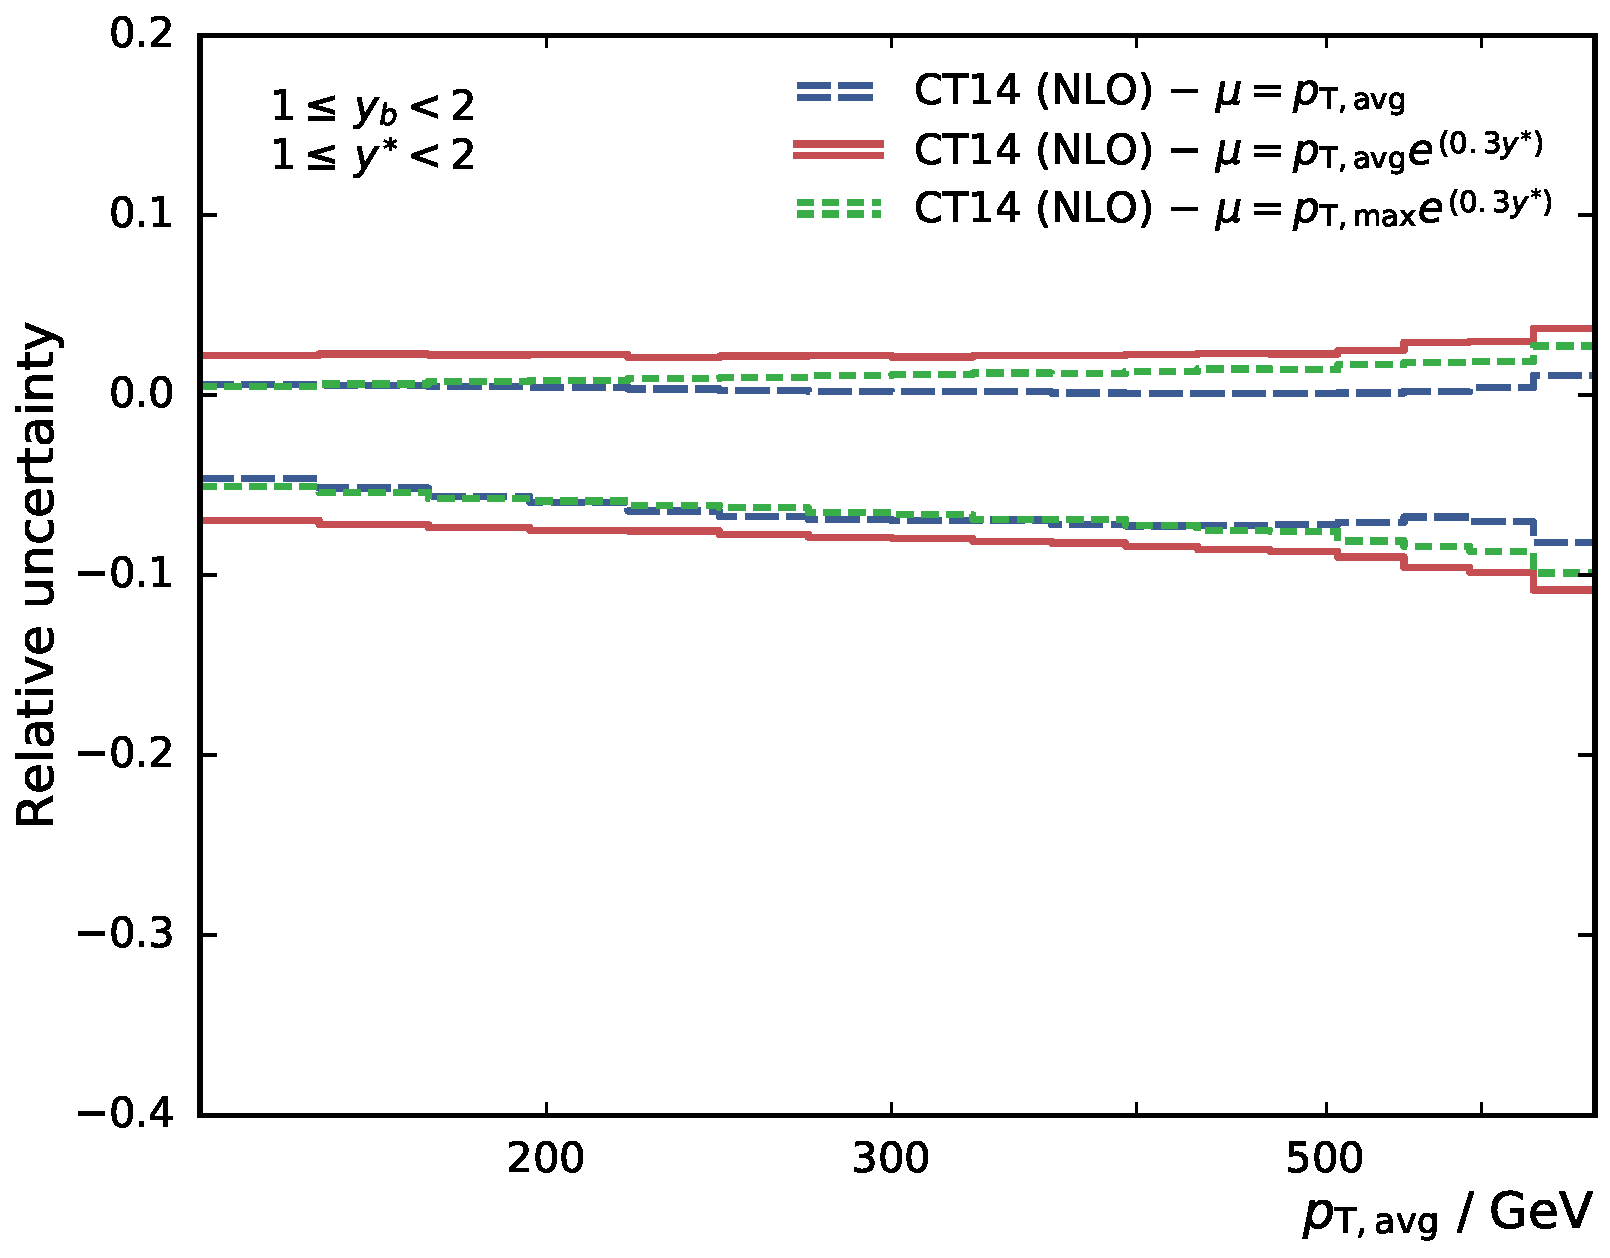
\includegraphics[width=0.45\textwidth]{figures/theory/scale_uncert_comp_yb1ys1.pdf}\hfill
    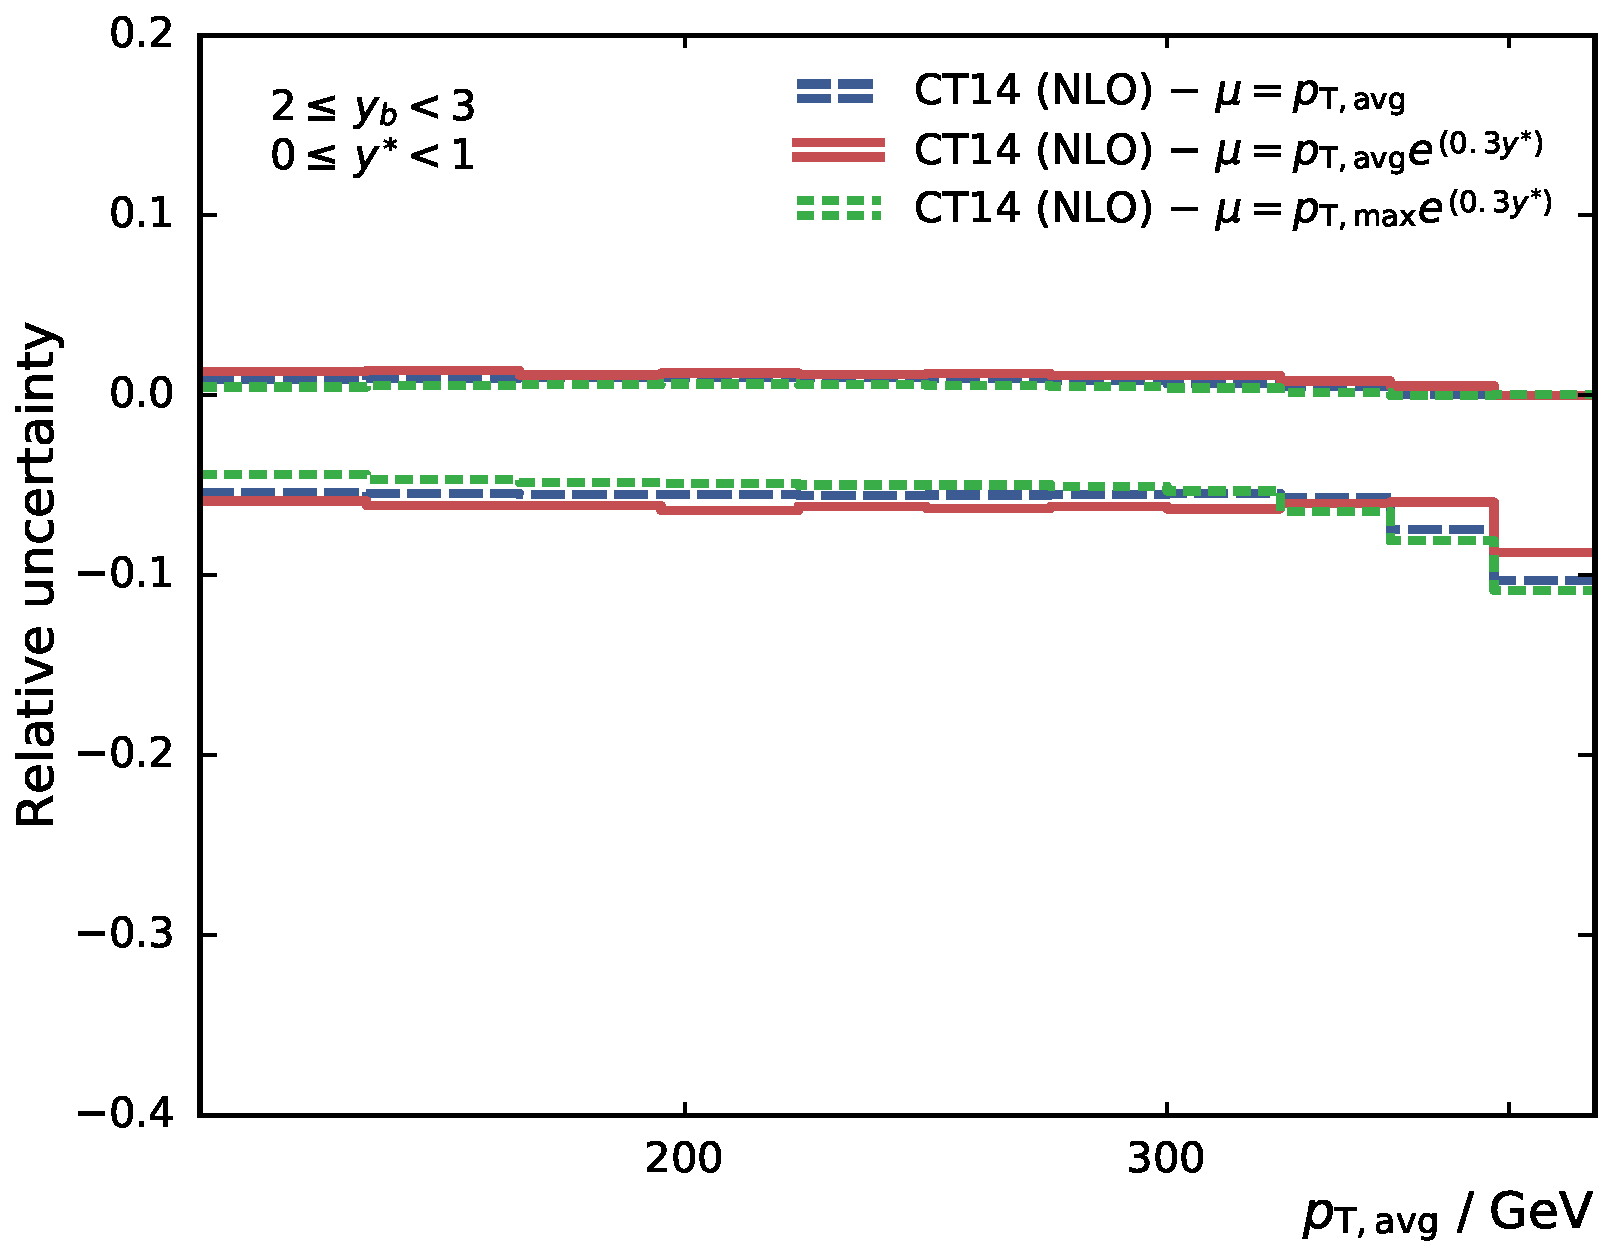
\includegraphics[width=0.45\textwidth]{figures/theory/scale_uncert_comp_yb2ys0.pdf}
    \caption{The scale uncertainty is estimated using the common approach of
        independently varying the renormalization and factorization scale
        choice in six independent combinations. The uncertainty is shown for the
        three investigated scale choices. In most cases the scale uncertainty is
        reasonable and of the size of 5\% to 10\%. In the high \ystar bin, the
        scale uncertainty of prediction with the \ptavg scale choice is
        undesirable large.}
    \label{fig:scale_uncertainties}
\end{figure}

\subsection{PDF uncertainties}

The dependence of the cross section calculation on the proton structure is
expressed in terms of parton distribution functions, which are derived from a
fit to data from different experiments. Different sources of
uncertainty affect the PDFs. These comprise the choice and the
functional form of the parametrization, the chosen theory model and input
parameters like the strong coupling constant \as or the quark masses and of
course also the uncertainties of the datapoints included in the PDFs.

When deriving the PDFs, all these uncertainties are taken into account and
propagated to the PDFs. The groups deriving the PDF sets provide prescriptions
how to evaluate these uncertainties. In Sec.~\ref{sec:nlo_comparisons} several
comparisons to predictions using the global PDF sets NNPDF 3.0, CT14 and
MMHT2014 are shown. In the following a short summary of the procedure to derive
the PDF uncertainties for each PDF set is given.

The NNPDF PDF set~\cite{Ball:2014uwa} uses a large number of pseudo experiments, in which the PDF
fit is performed using data smeared within their uncertainties taking into
account all correlations. These so-called replicas are averaged to give the
central result and the spread of the replicas determines the uncertainty. The
symmetric PDF uncertainty $\Delta X^\pm$ of a quantity $X$ which can be a cross section calculation or
even the PDF itself is expressed as

\begin{equation*}
    \Delta X^{\pm} = \sqrt{\frac{1}{N-1} \sum_{i=1}^N \left[ X_{i} - X_{\mathrm{central}} \right]^2}
\end{equation*}
where $N$ denotes the number of replicas.

The CT14 PDF set ~\cite{Dulat:2015mca} and the MMHT2014 PDF set~\cite{Harland-Lang:2014zoa} both
employ the eigenvector method to encode the uncertainties. A transformation from
the parameter basis to the eigenvector basis is done to yield mutually
uncorrelated eigenvectors. By varying the eigenvectors upwards and downwards, a
set of eigenvector pairs is generated which can be used to determine the asymmetric
uncertainty $\Delta X^+$ and $\Delta X^-$ of a quantity $X$. $X_0$ depicts the
central prediction, $X_i^{\mathrm{up}}$ and $X_i^{\mathrm{dn}}$ the prediction
using the upwards and downvards variation of the eigenvector PDF set $i$ and
$N_{\mathrm{EV}}$ the number of eigenvectors in the PDF set.

\begin{equation*}
\begin{aligned}
    \Delta X^+ &= \sqrt{\sum_i^{N_{\mathrm{EV}}} \left[ \max(X_i^{\mathrm{up}}
    -X_0, X_i^{\mathrm{dn}} - X_0, 0)\right]^2}\\
\Delta X^- &= \sqrt{\sum_i^{N_{\mathrm{EV}}} \left[ \min(X_i^{\mathrm{up}} - X_0, X_i^{\mathrm{dn}} - X_0,0)\right]^2}
\end{aligned}
\end{equation*}

The symmetric uncertainty $\Delta X^{\pm}$ is given by half the difference of the upwards and
downwards variation.

\begin{equation*}
    \Delta X^{\pm} = \sqrt{\sum_i^{N_{\mathrm{EV}}} \left[ \frac{X_i^+ -
    X_i^-}{2} \right]^2}
\end{equation*}

The uncertaintiy afflicted to the CT14 PDF set describes a 90\% confidence
interval while the MMHT and NNPDF PDF uncertainties represent a 68\% confidence
interval. The CT14 uncertainties are scaled to 68CL using $s = \sqrt{2}
\erf^{-1}(0.9) = 1.645$.

Fig.~\ref{fig:pdf_uncertainties} shows the fractional PDF uncertainty for the
three global PDF sets discussed. The PDF uncertainty in the bins with small
\ystar and small \yboost values is comparably small. This is due to the fact
that mostly events with two jets which are balanced in rapidity contribute, in
which the medium $x$ region of the proton PDFs is accessed which are well known
already. The PDF uncertainty of the cross section for high values of \ystar and
low values of \yboost, in which two forward jets are on opposite sides of the
detector is also relatively small. Most interestingly the uncertainty strongly
increases for the bin with large values of \yboost and small values of \ystar.
Especially in the high-\pt region the uncertainty is sizeable. To achieve a high
boost of the dijet system and a high \ptavg value, the protons must be accessed
in the high-$x$ region which is not well determined up to now and is afflicted
with large PDF uncertainties. Especially the NNPDF PDF set has a large
uncertainty in this region. This is caused by the very flexible parametrization
of the NNPDF PDF set which results in large PDF uncertainty in phase space
regions not covered by data.

\begin{figure}[htp]
    \centering
    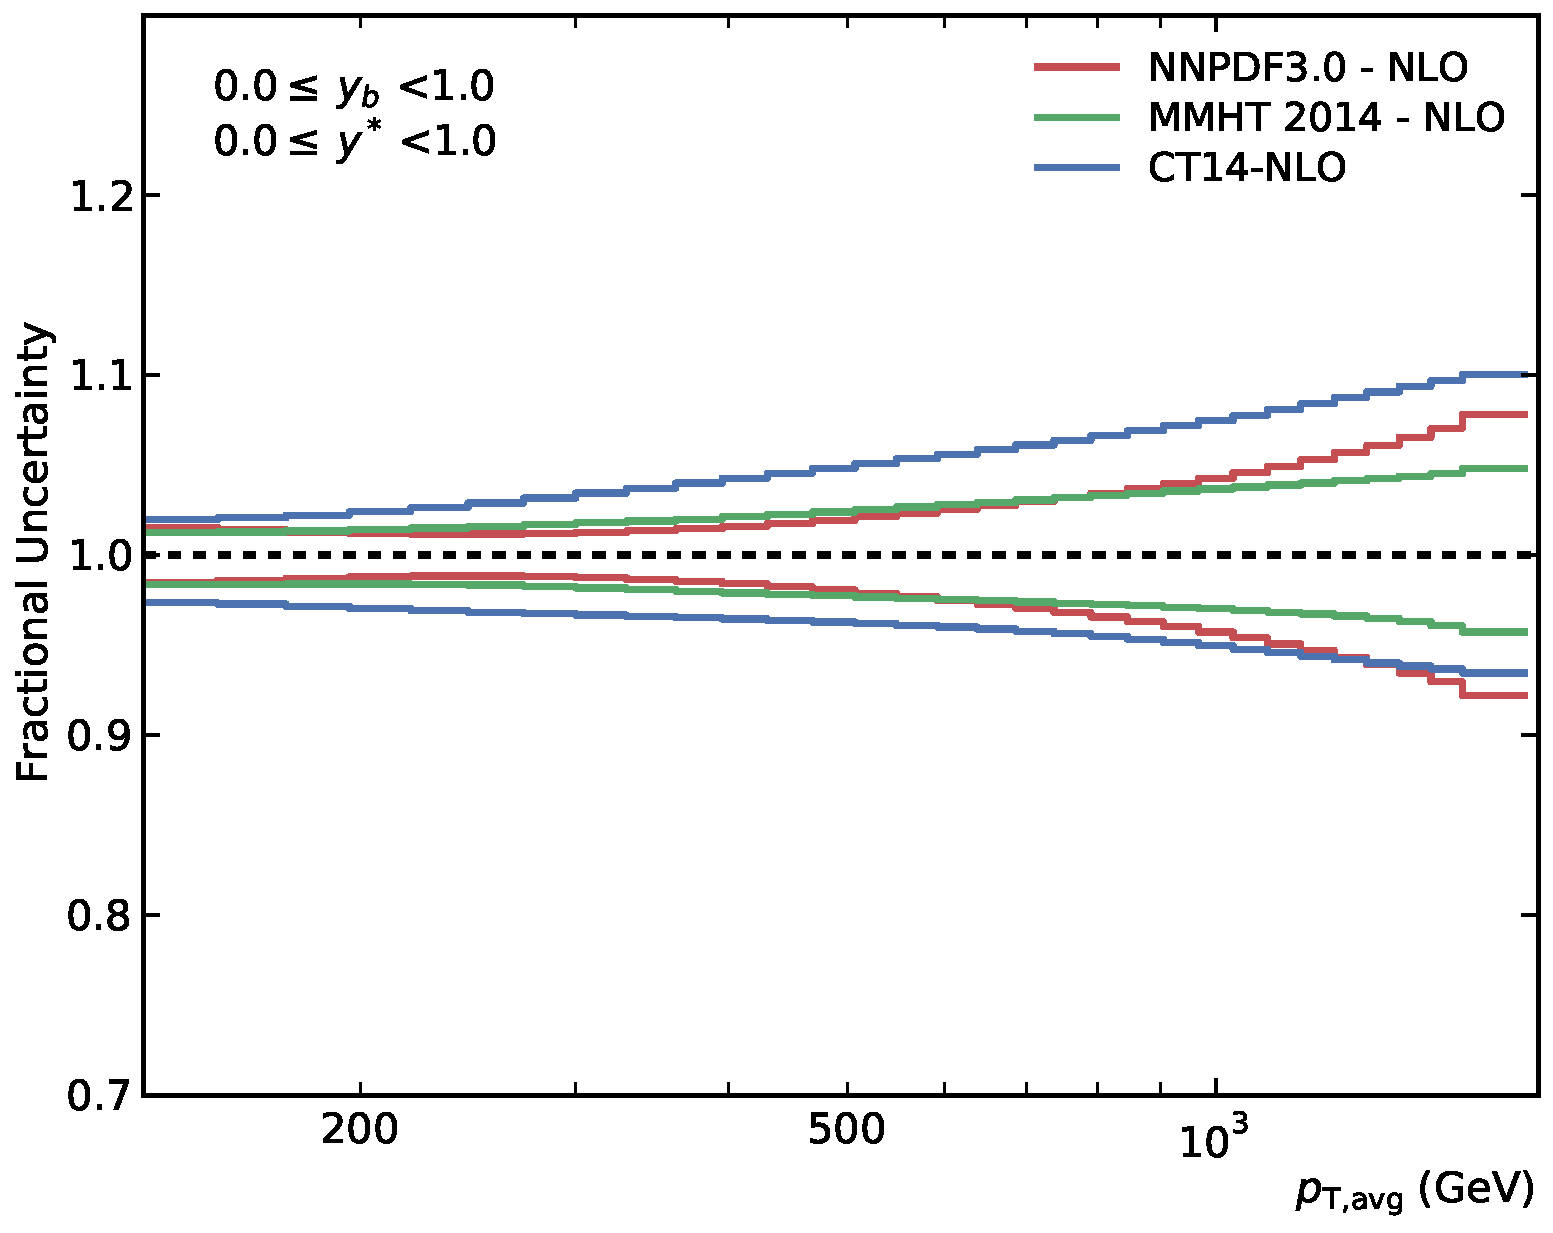
\includegraphics[width=0.45\textwidth]{figures/theory/pdf_unc_comparison_yb0ys0.pdf}\hfill
    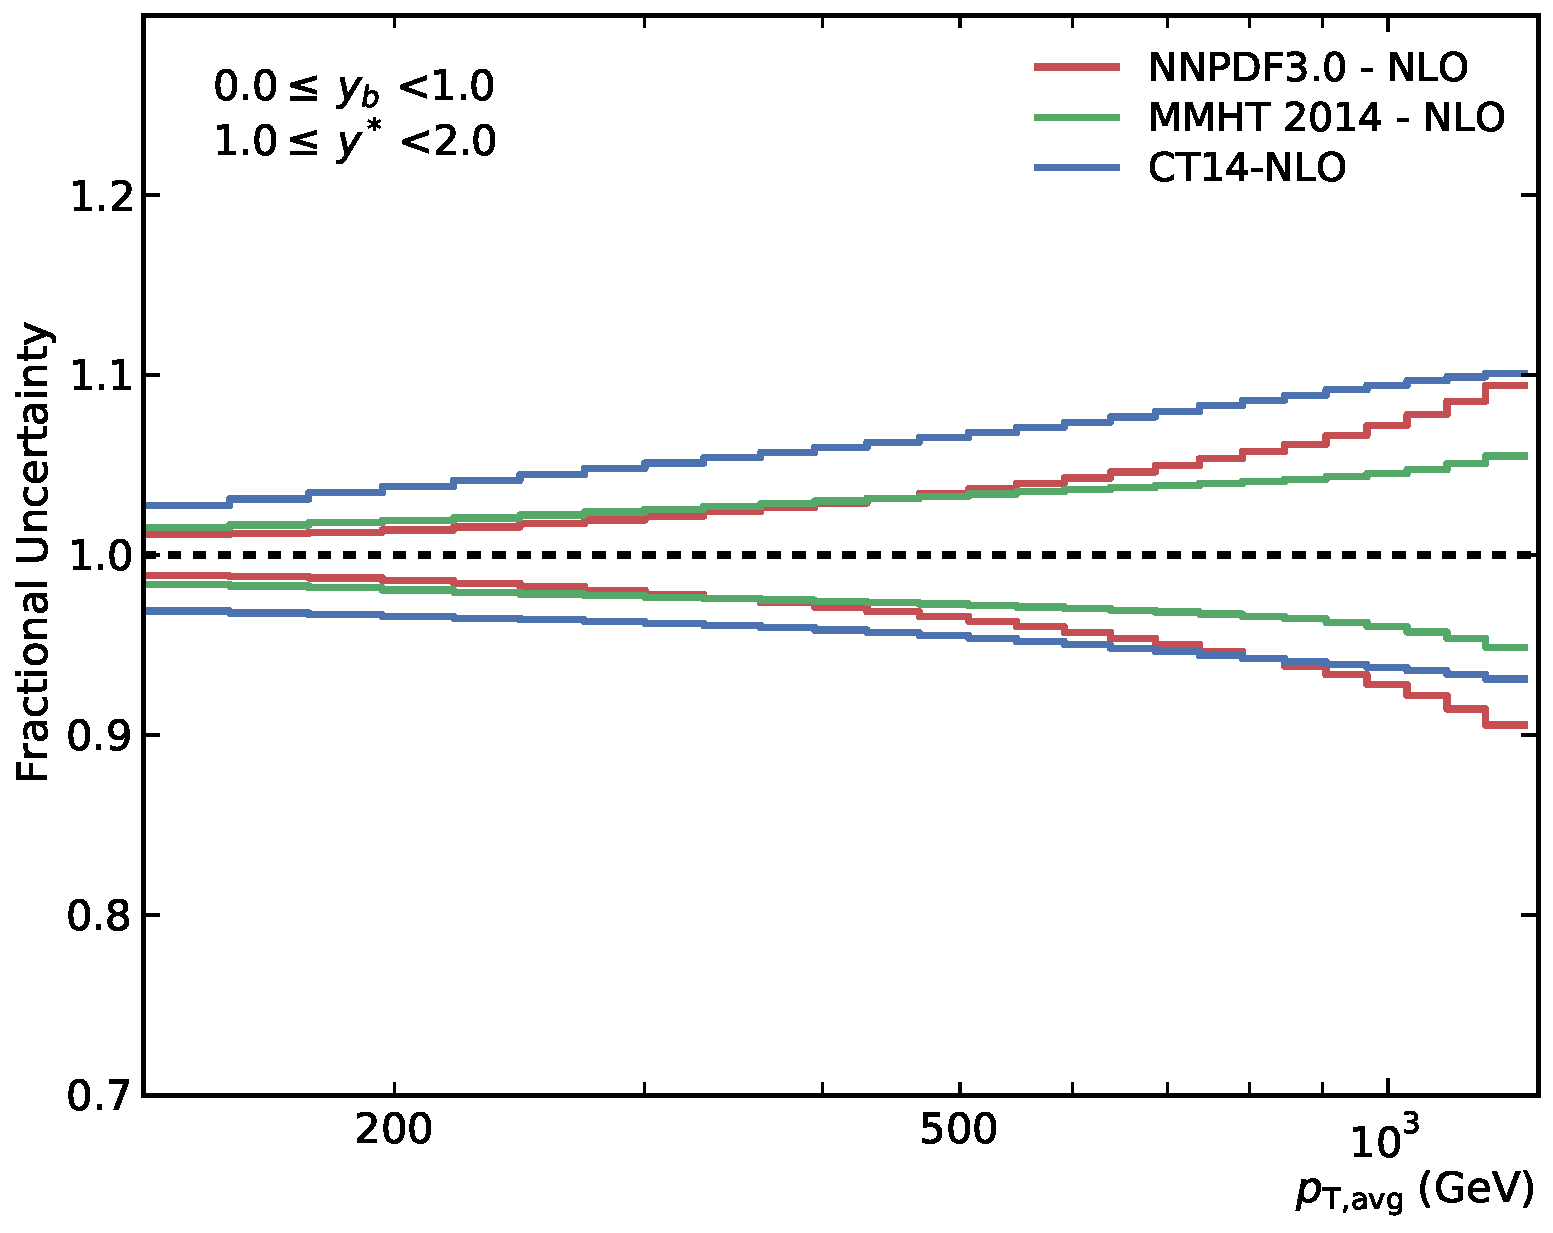
\includegraphics[width=0.45\textwidth]{figures/theory/pdf_unc_comparison_yb0ys1.pdf}
    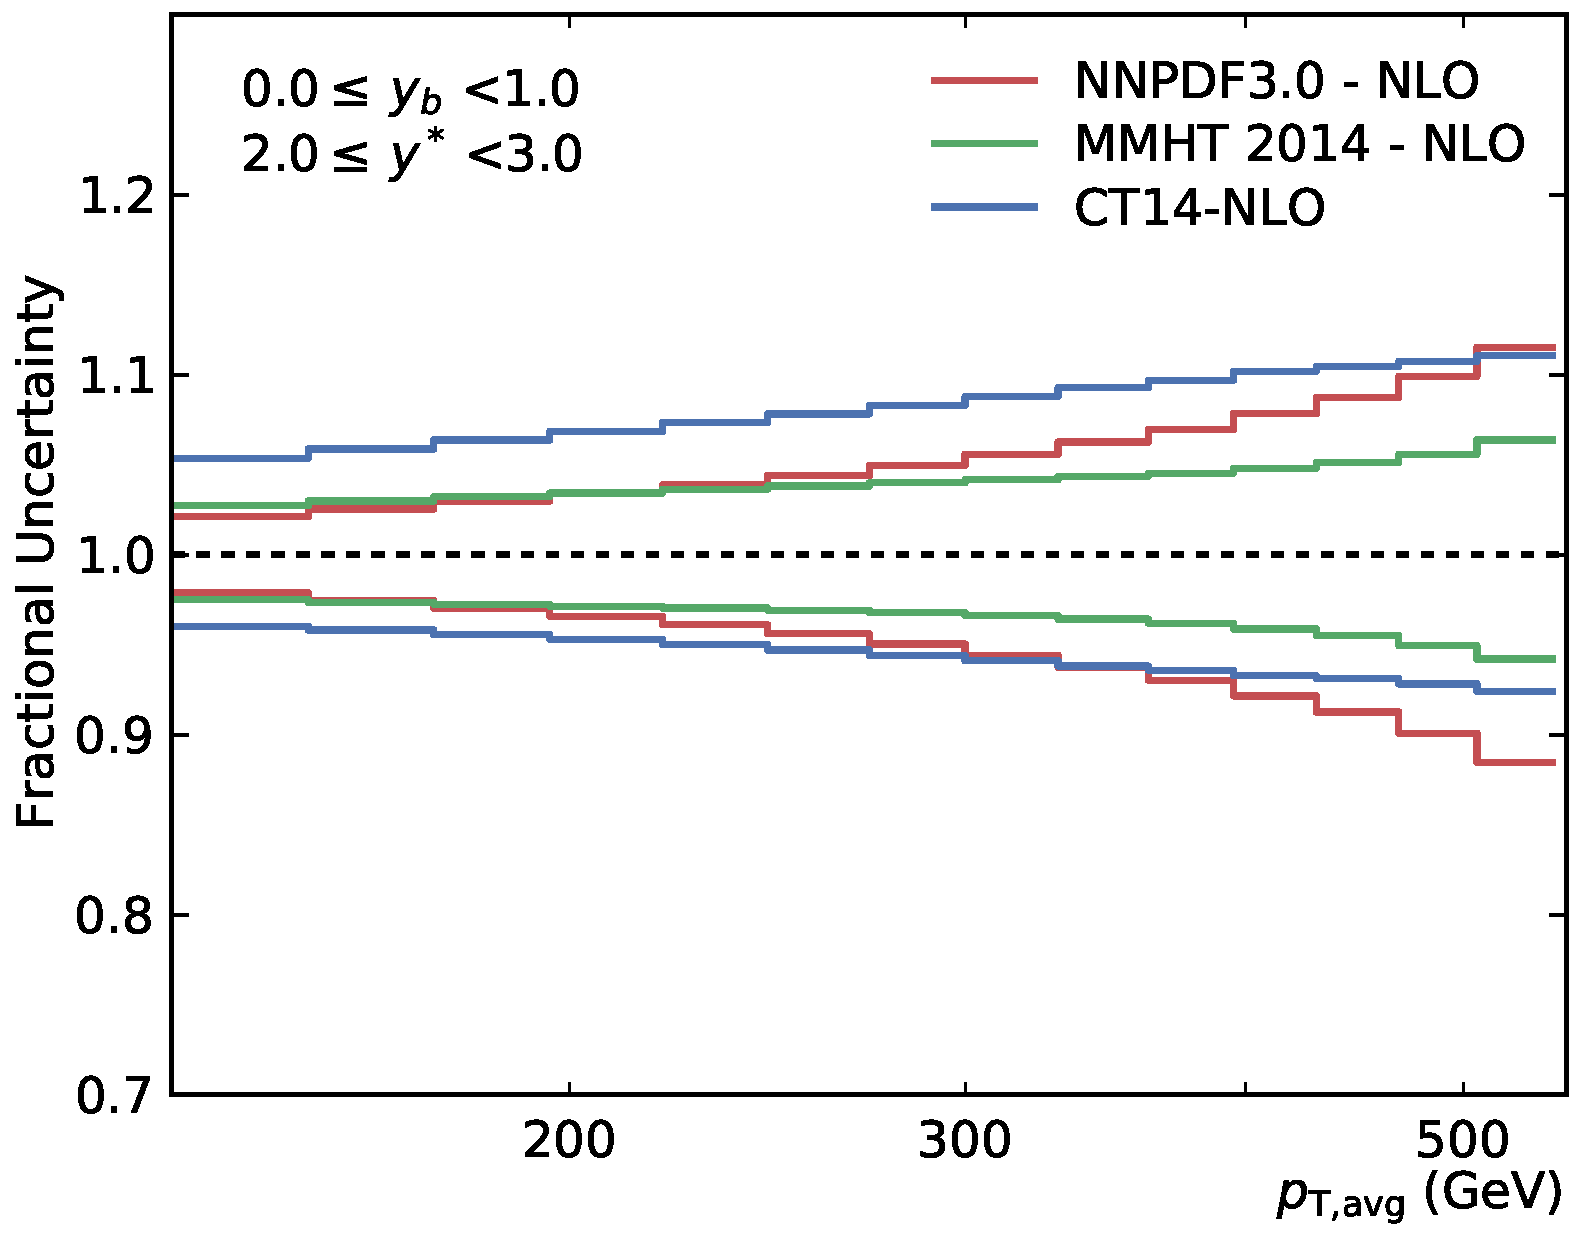
\includegraphics[width=0.45\textwidth]{figures/theory/pdf_unc_comparison_yb0ys2.pdf}\hfill
    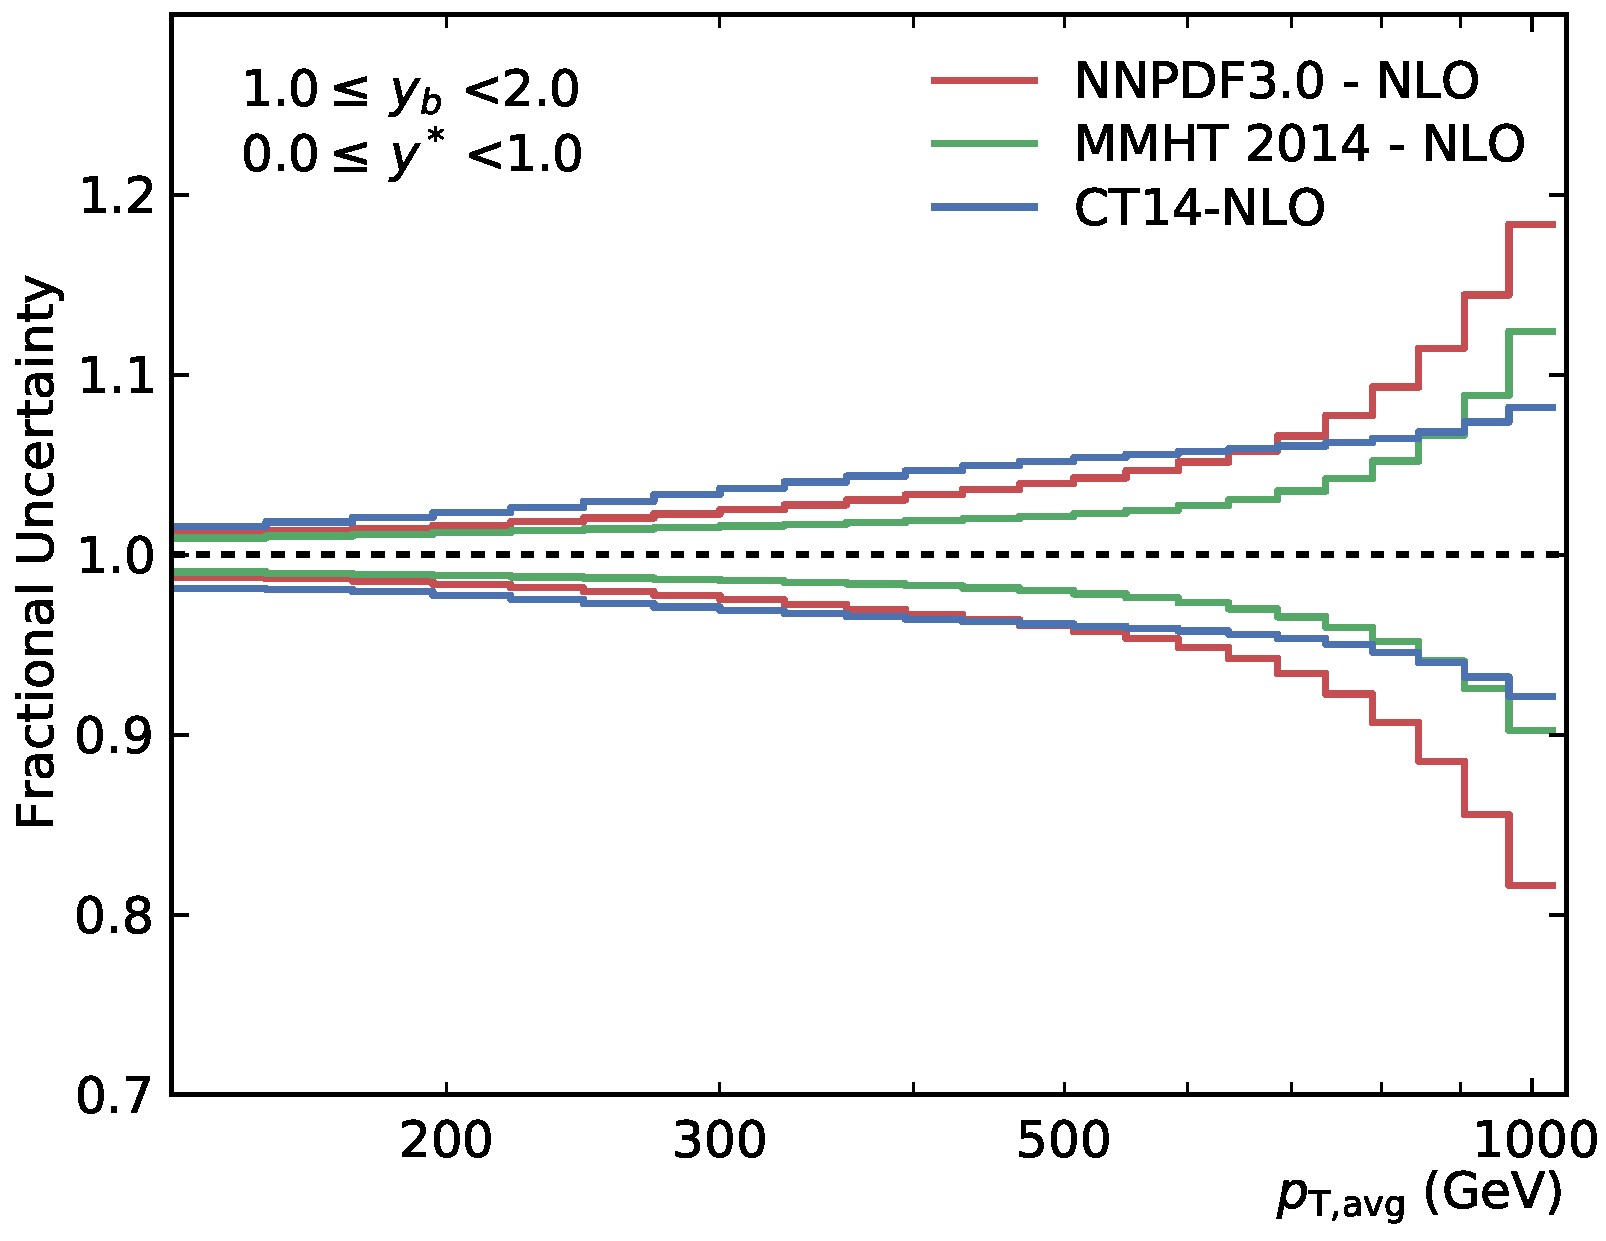
\includegraphics[width=0.45\textwidth]{figures/theory/pdf_unc_comparison_yb1ys0.pdf}
    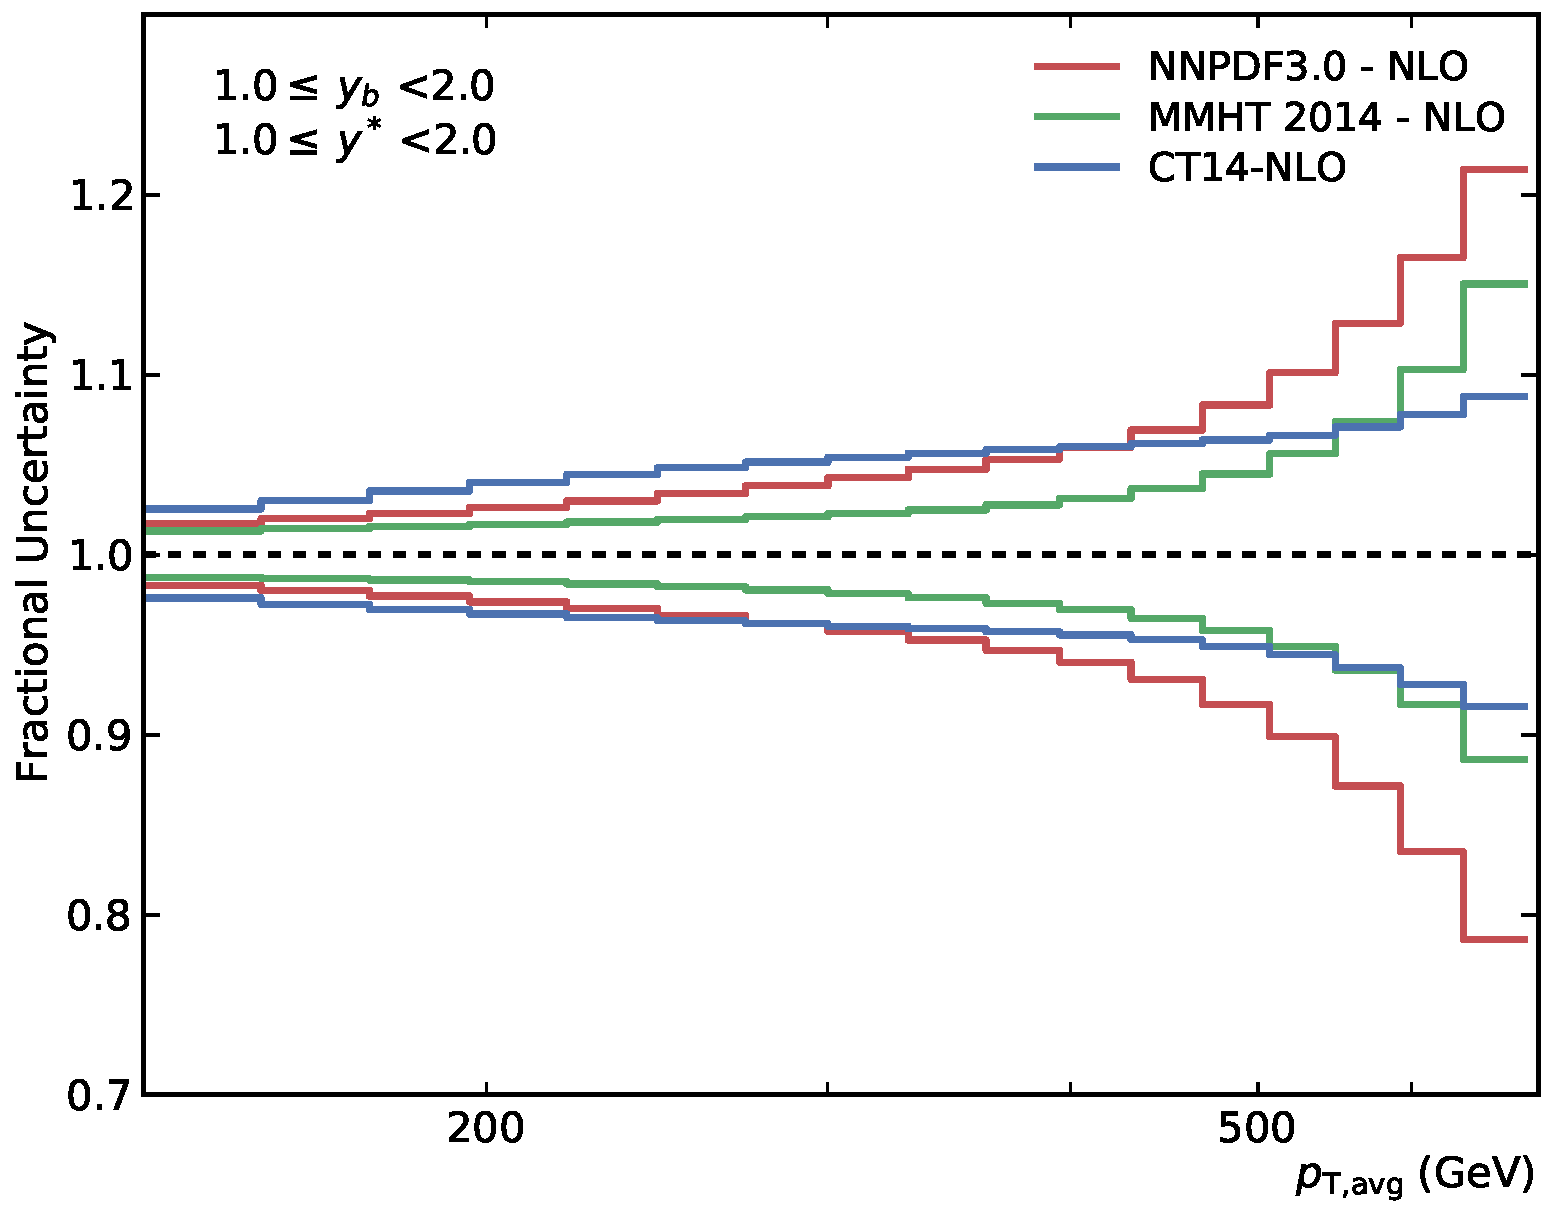
\includegraphics[width=0.45\textwidth]{figures/theory/pdf_unc_comparison_yb1ys1.pdf}\hfill
    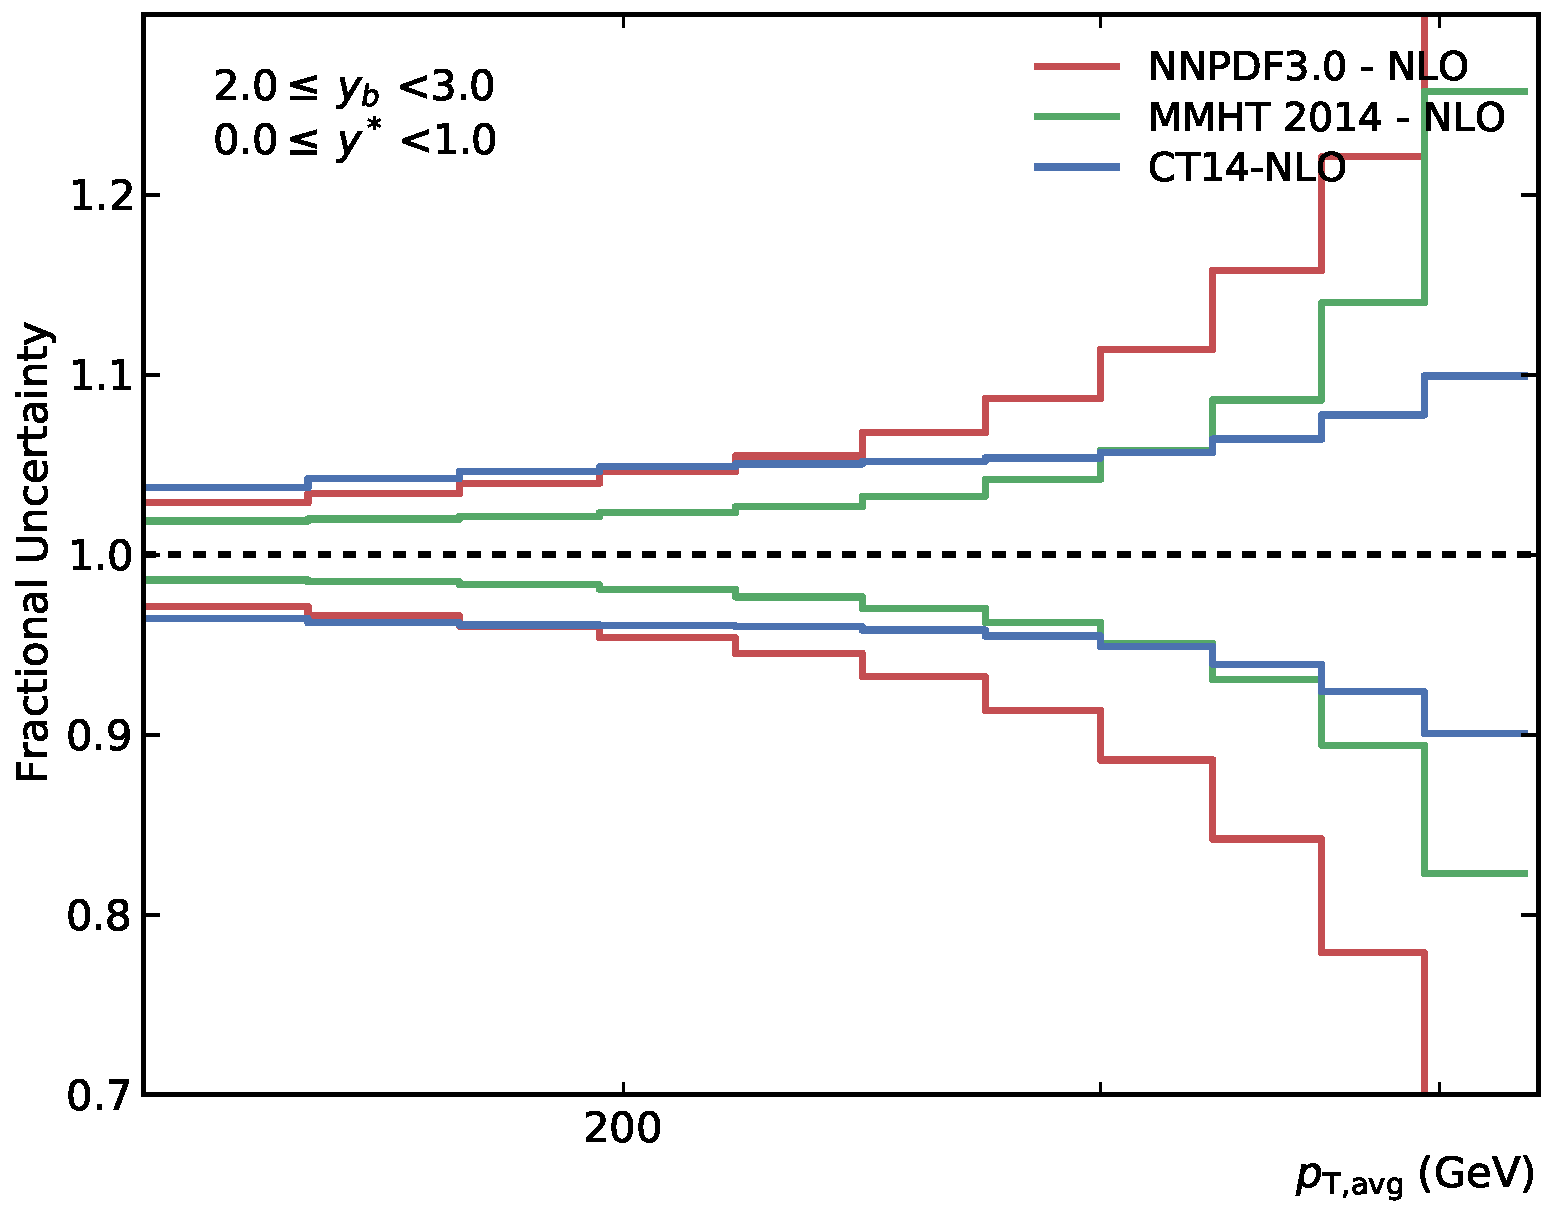
\includegraphics[width=0.45\textwidth]{figures/theory/pdf_unc_comparison_yb2ys0.pdf}
    \caption{The relative PDF uncertainty calculated using the three PDF sets
    NNDFP 3.0, CT14 and MMHT 2014. The uncertainty represents a 68\% confidence
    interval. The PDF uncertainty is sizeable especially in the forward region in
    which both jets have the same sign and high fractional proton momenta are
    accessed. }
    \label{fig:pdf_uncertainties}
\end{figure}

\begin{figure}[htp]
    \centering
    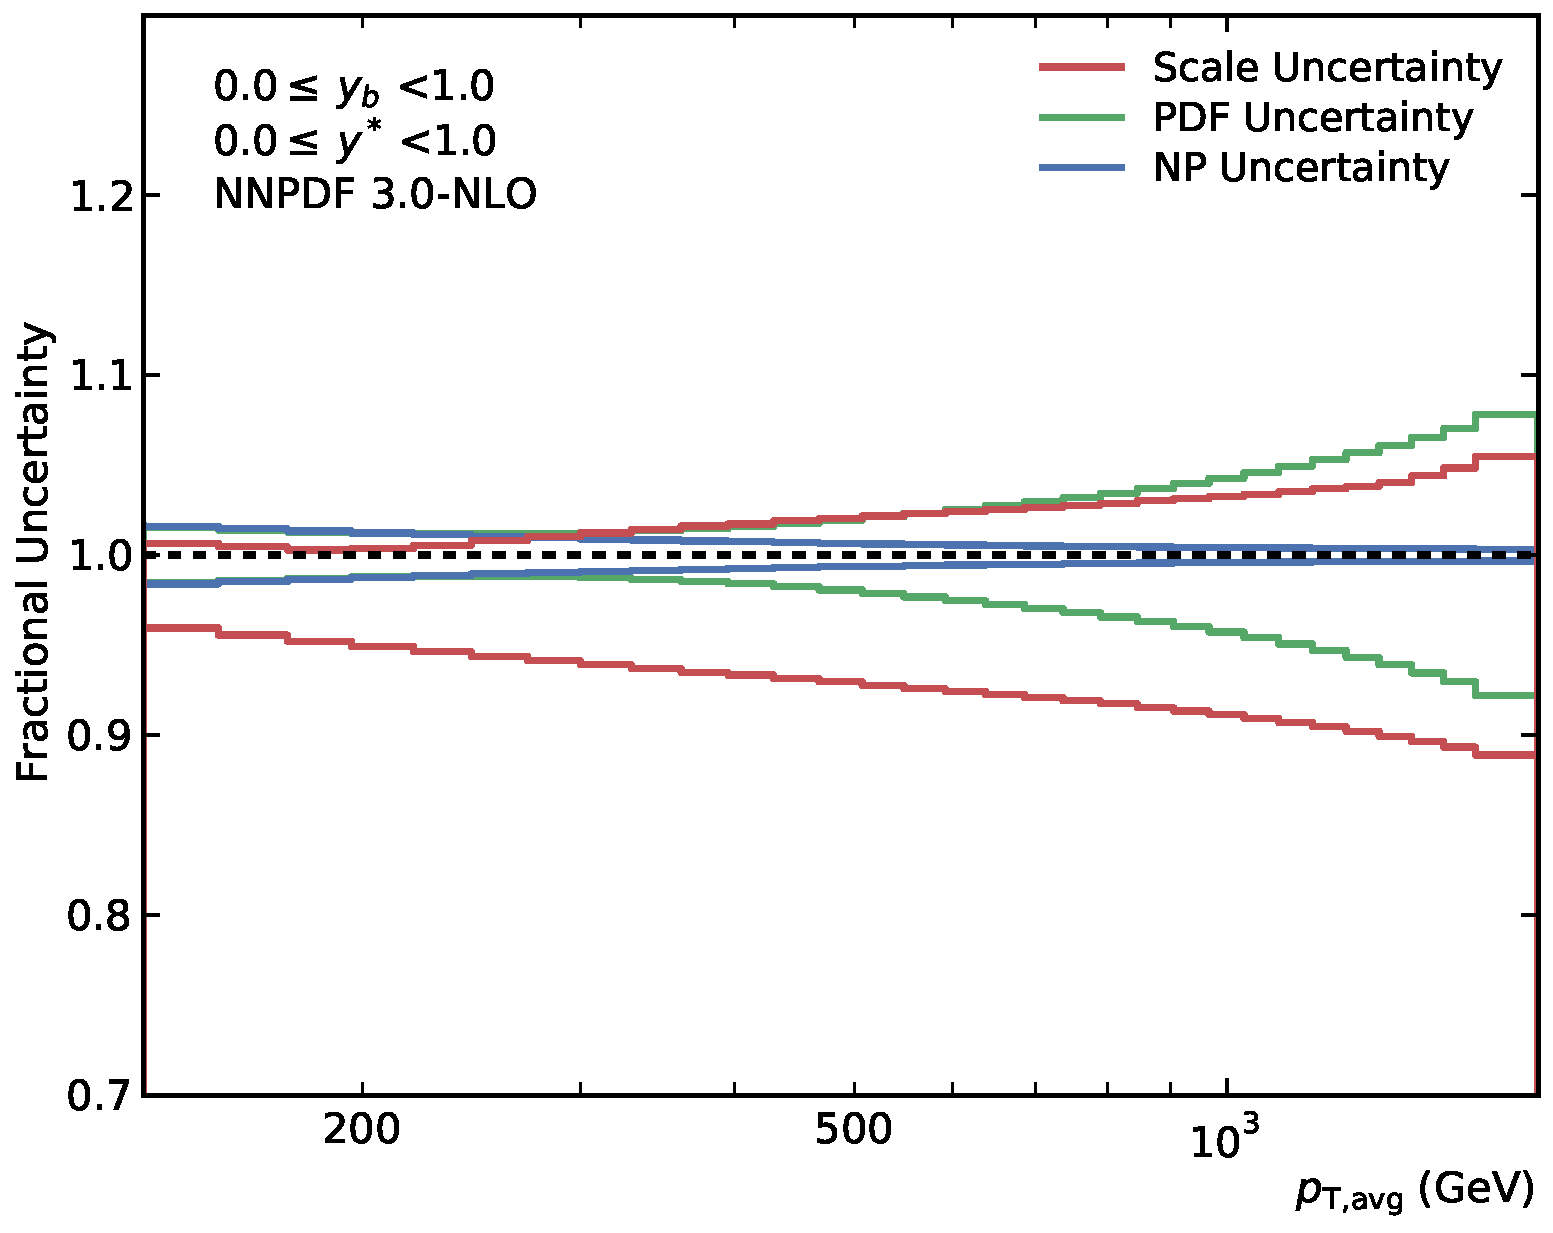
\includegraphics[width=0.45\textwidth]{figures/theory/theo_unc_yb0ys0.pdf}\hfill
    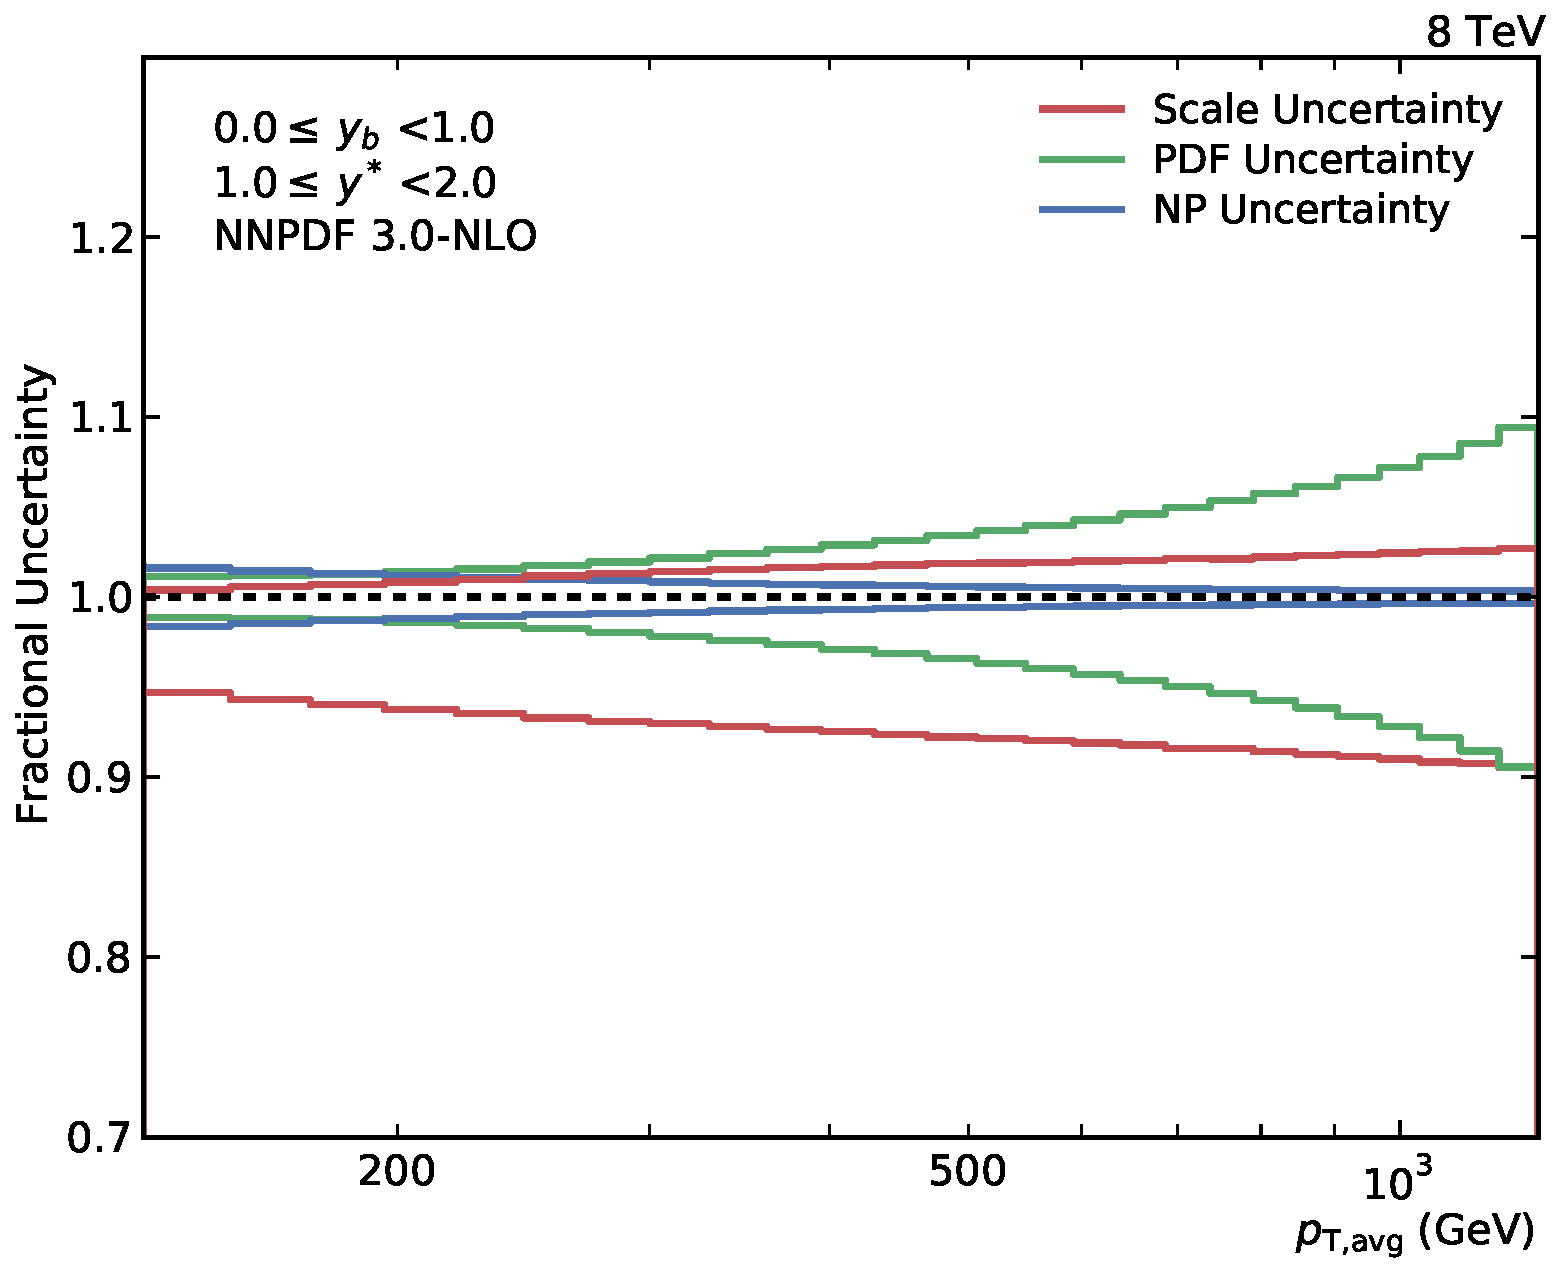
\includegraphics[width=0.45\textwidth]{figures/theory/theo_unc_yb0ys1.pdf}
    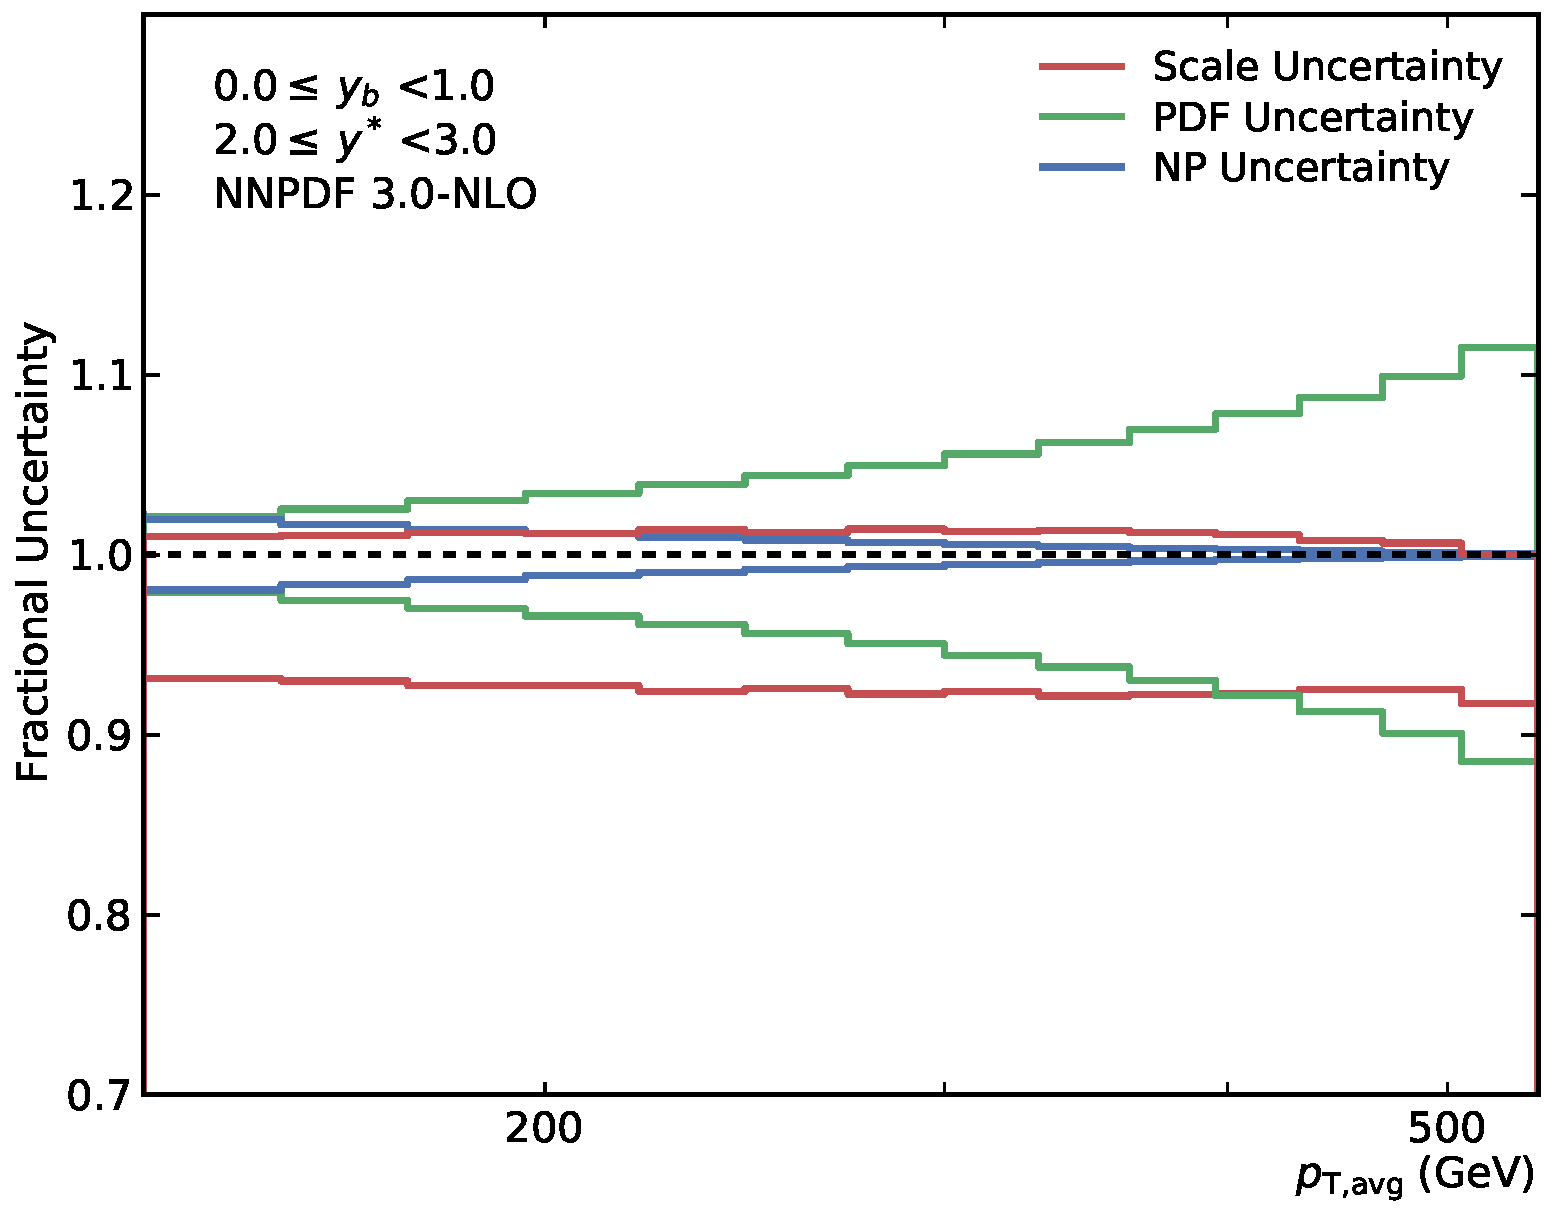
\includegraphics[width=0.45\textwidth]{figures/theory/theo_unc_yb0ys2.pdf}\hfill
    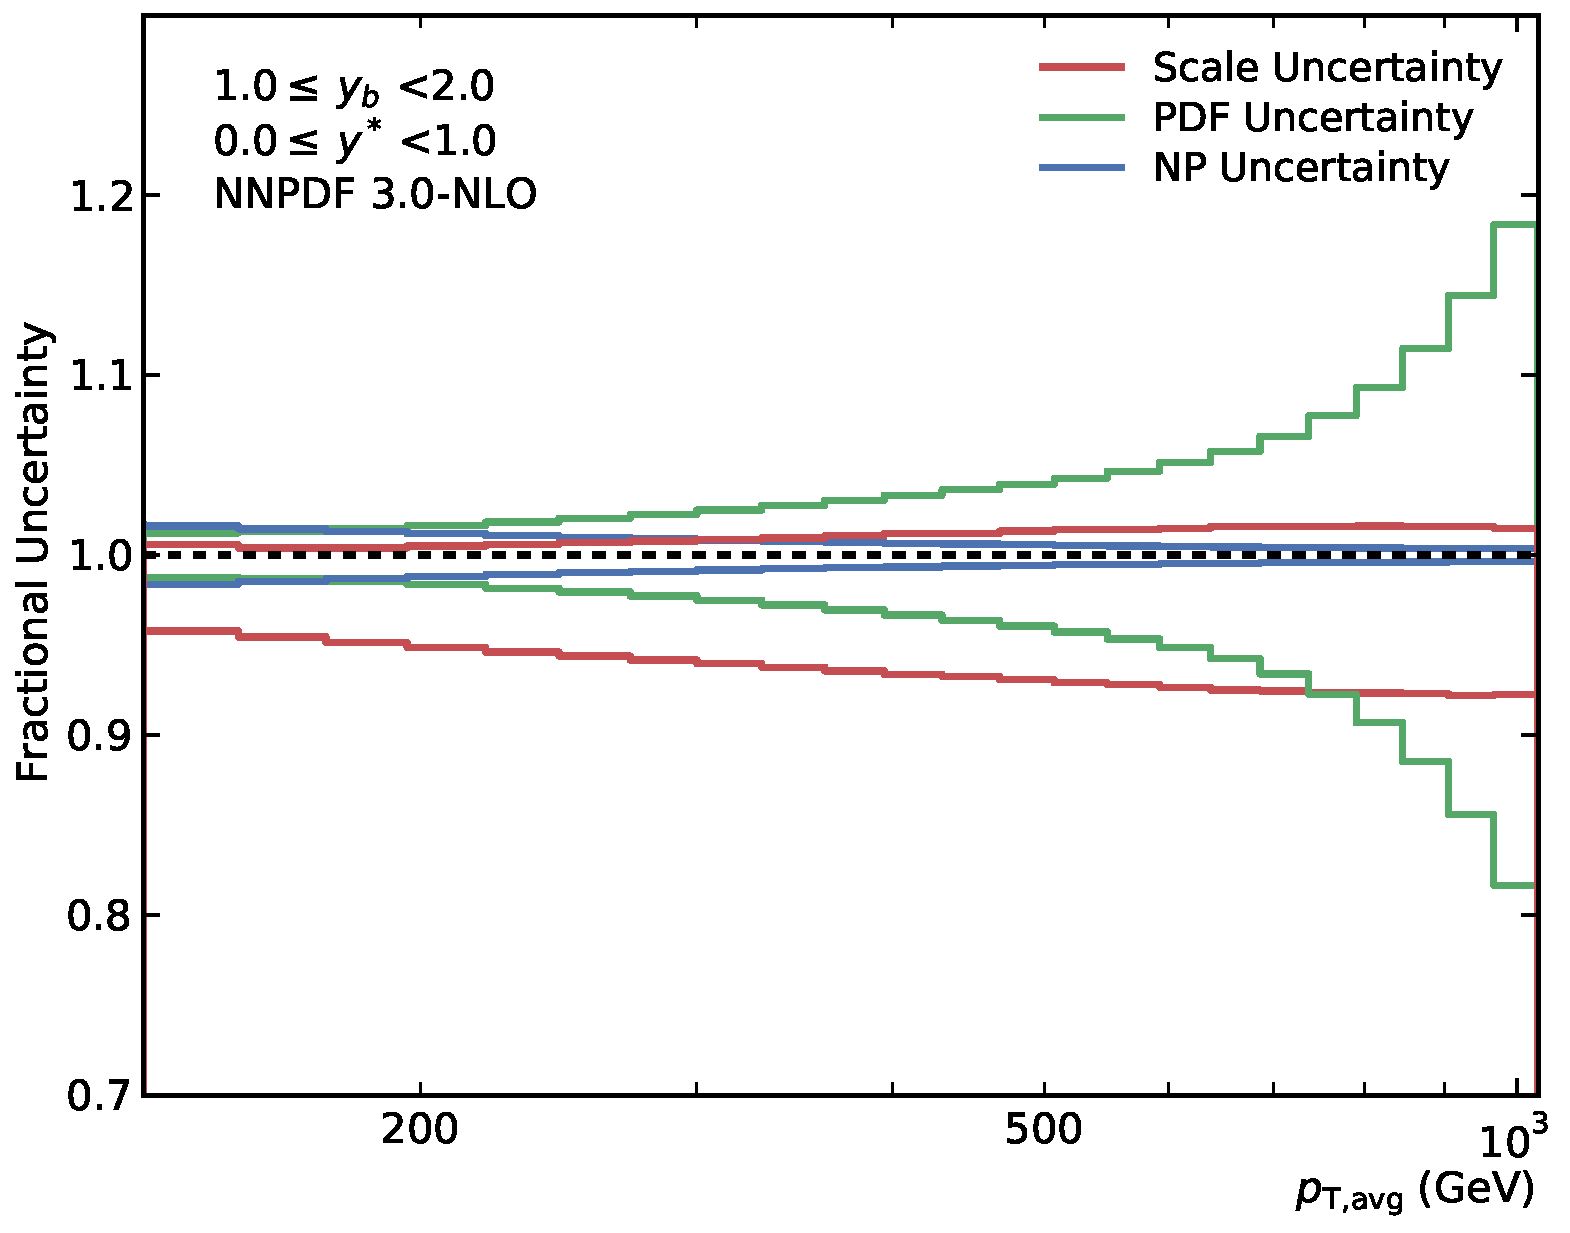
\includegraphics[width=0.45\textwidth]{figures/theory/theo_unc_yb1ys0.pdf}
    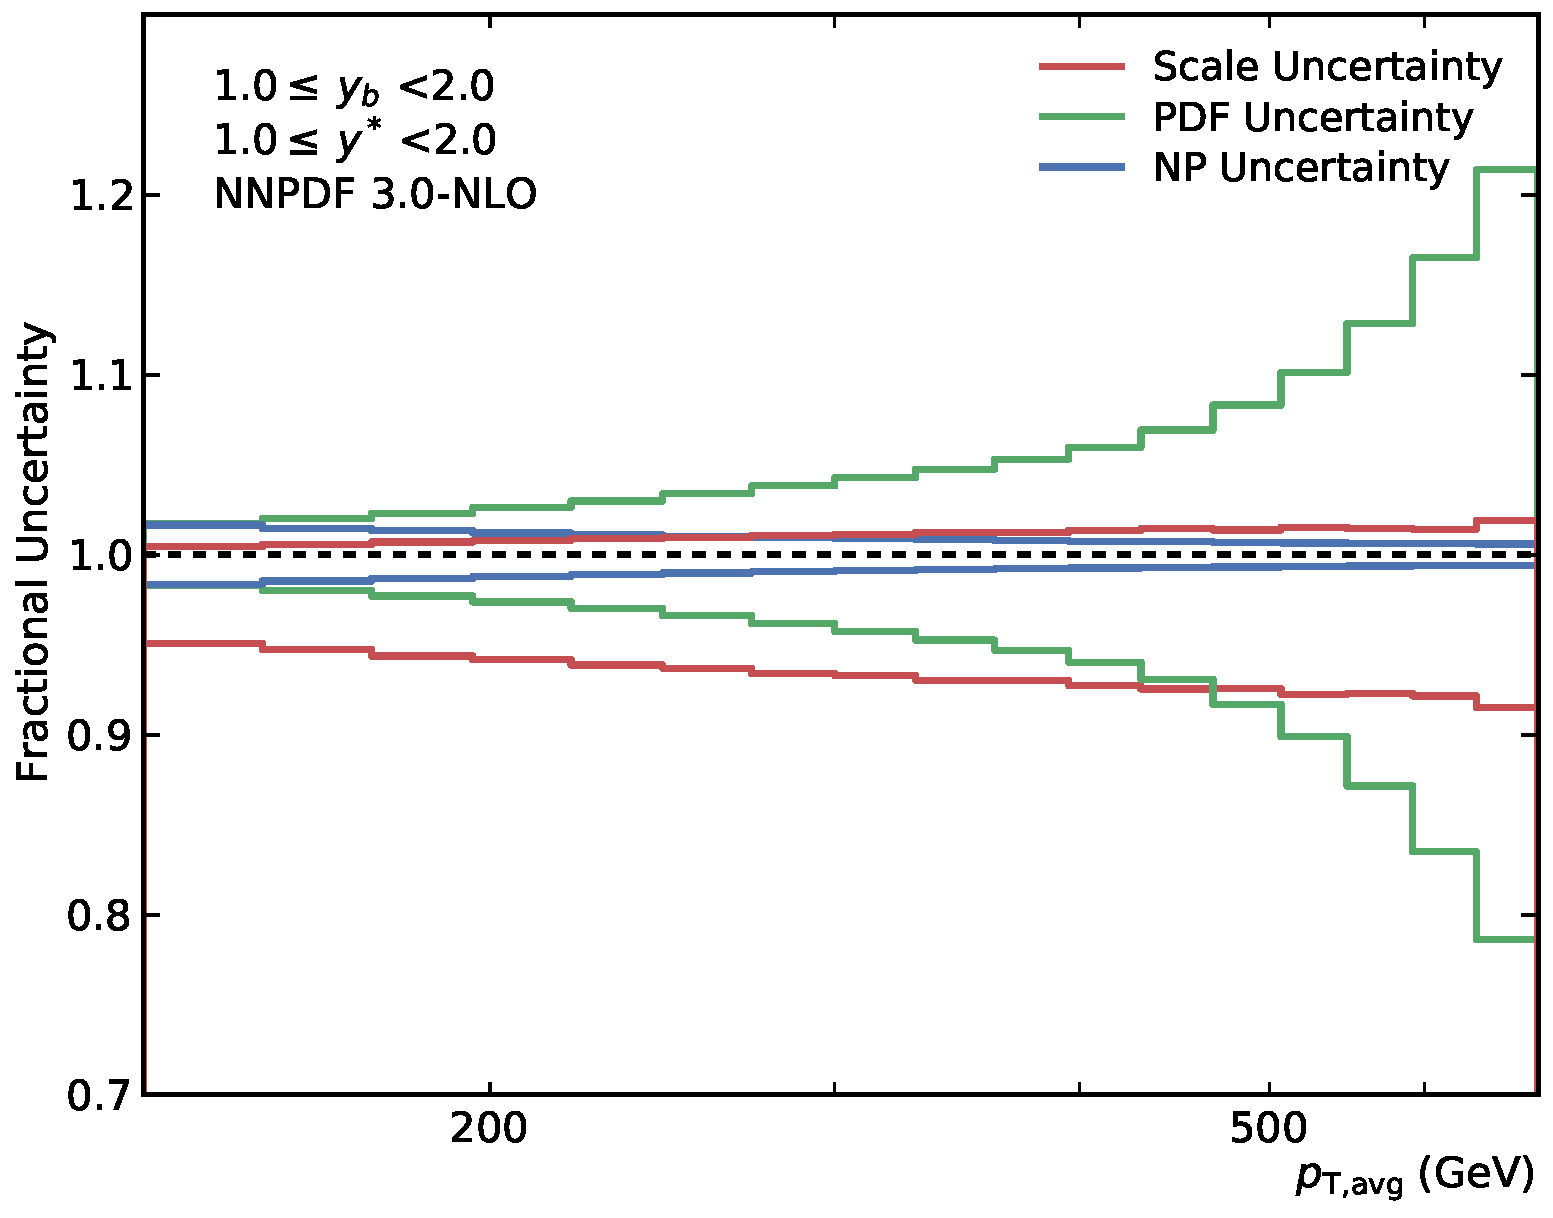
\includegraphics[width=0.45\textwidth]{figures/theory/theo_unc_yb1ys1.pdf}\hfill
    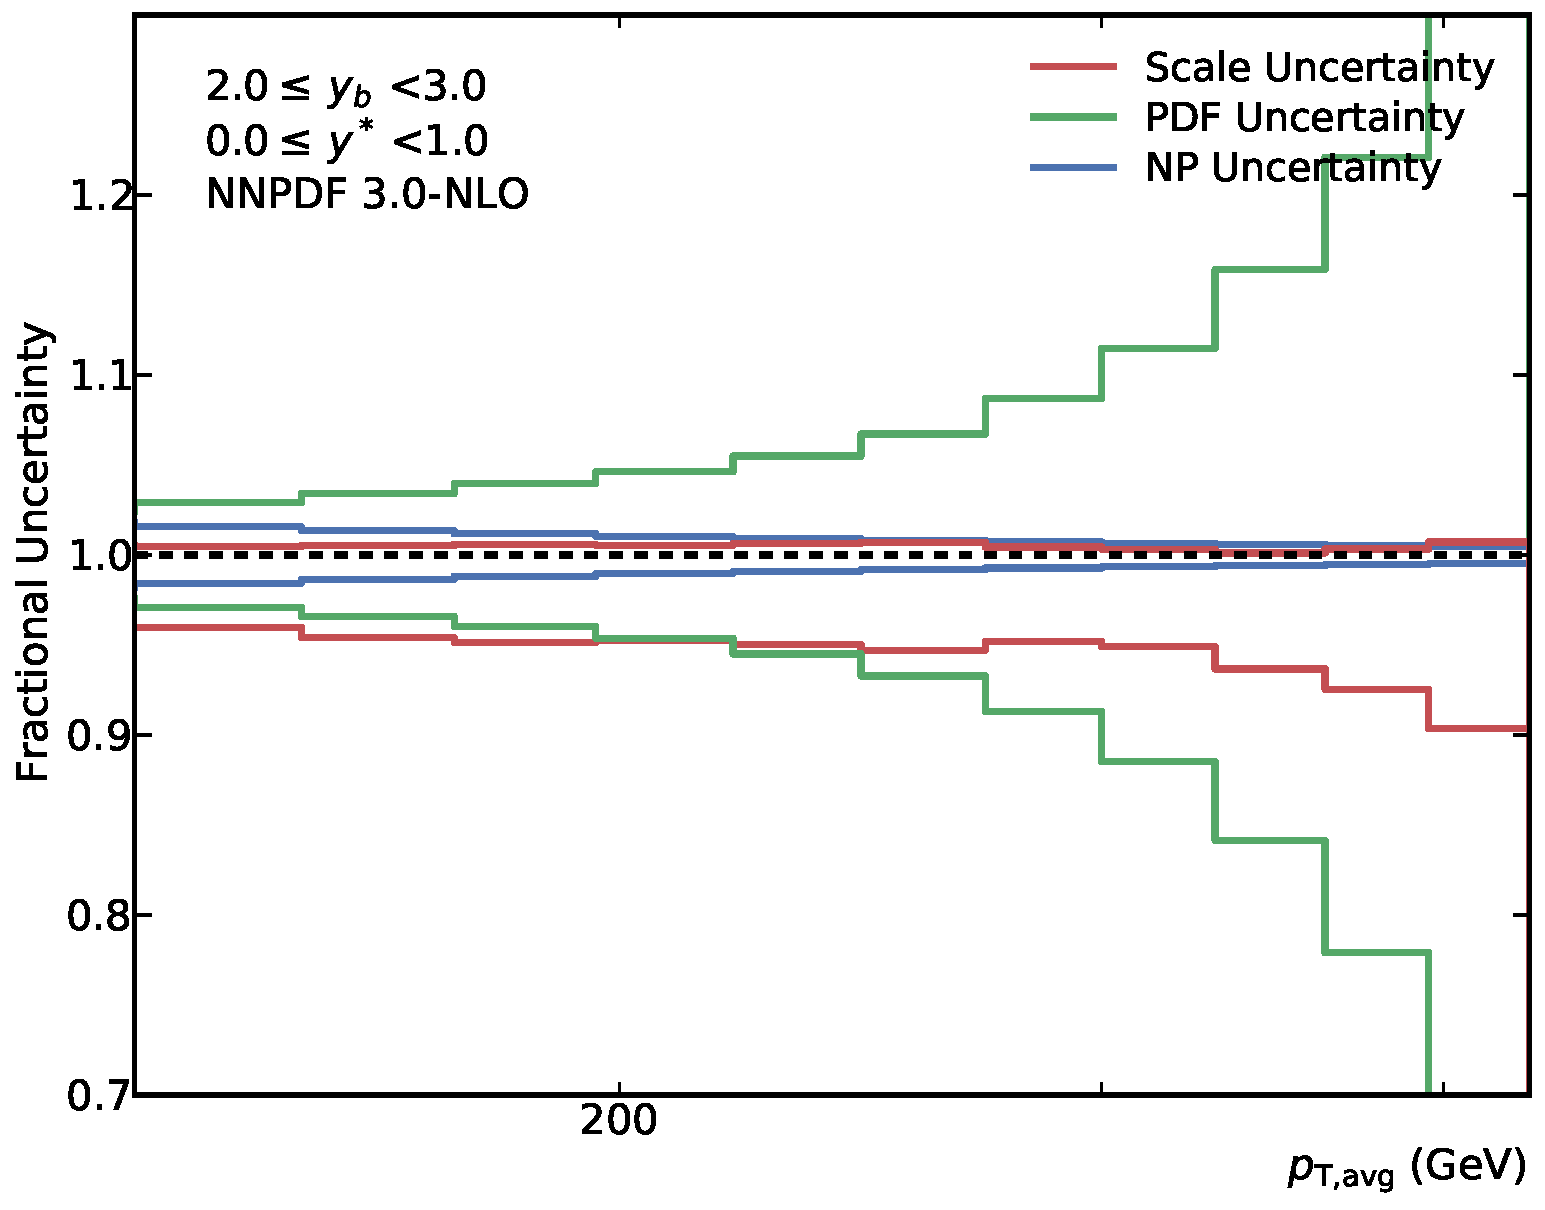
\includegraphics[width=0.45\textwidth]{figures/theory/theo_unc_yb2ys0.pdf}
    \caption{Overview of the theoretical uncertainties of the NLO prediction.
    The scale uncertainty is the dominant uncertainty in the low-\pt region. At
high-\pt and especially in the forward region, the PDF uncertainty becomes
dominant. The NP uncertainty is sizeable only in low-\pt region and becomes
negligible at higher \pt when the NP correction approaches unity.}
    \label{fig:theo_uncertainties}
\end{figure}
